\documentclass[11pt]{article}
\usepackage[margin=1in]{geometry}
\usepackage[T1]{fontenc}
\usepackage{lmodern}
\usepackage{amsmath}
\usepackage{mathtools}
\usepackage{amssymb}
\usepackage{amsthm}
\usepackage{microtype}
\usepackage{enumitem}
\usepackage{tikz}
\usetikzlibrary{arrows.meta,positioning,calc}
\usepackage{natbib}
\usepackage[colorlinks=true,linkcolor=blue!50!black,citecolor=green!35!black,urlcolor=blue!60!black]{hyperref}

% Operators (as in the original note)
\newcommand{\diag}{\operatorname{diag}}
\newcommand{\Hom}{\operatorname{Hom}}
\newcommand{\rank}{\operatorname{rank}}
\newcommand{\Supp}{\operatorname{Supp}}

% Additional notation
\newcommand{\R}{\mathbb{R}}
\newcommand{\E}{\mathbb{E}}
\newcommand{\Sym}{\operatorname{Sym}}
\newcommand{\GL}{\mathrm{GL}}
\newcommand{\col}{\operatorname{col}}
\newcommand{\vect}{\operatorname{vec}}
\newcommand{\rankcp}{\operatorname{rank}_{\mathrm{CP}}}
\newcommand{\ip}[2]{\langle #1,#2\rangle}
\newcommand{\norm}[1]{\lVert #1\rVert}
\newcommand{\xb}{\bar{x}}
\newcommand{\hb}{\bar{h}}
\newcommand{\cb}{\bar{c}}
\newcommand{\Eint}{E_{\mathrm{int}}}
\newcommand{\Eext}{E_{\mathrm{ext}}}
\newcommand{\Lhat}{\widehat{\mathcal L}}
\newcommand{\fhat}{\hat f}
\newcommand{\Cov}{\operatorname{Cov}}
\newcommand{\Var}{\operatorname{Var}}

% Theorem-like environments (definition style, as in the original note)
\theoremstyle{definition}
\newtheorem{theorem}{Theorem}[section]
\newtheorem{proposition}[theorem]{Proposition}
\newtheorem{lemma}[theorem]{Lemma}
\newtheorem{corollary}[theorem]{Corollary}
\newtheorem{definition}[theorem]{Definition}
\newtheorem{remark}[theorem]{Remark}
\newtheorem{example}[theorem]{Example}
\newtheorem{question}[theorem]{Question}
\newtheorem{hypothesis}[theorem]{Hypothesis}
\numberwithin{equation}{section}

\title{Tensor networks as surrogate models of training dynamics}
\author{}
\date{Research note, \today}

\begin{document}
\maketitle

\begin{abstract}
This note motivates tree tensor networks (TTNs) as surrogate models of the training dynamics of deep neural networks, and makes the underlying mathematics precise. We define tensor networks, TTNs, their edge matricizations, hierarchical ranks and hierarchical singular value decomposition (HSVD), and compare the relevant notions of tensor rank. A deep network with polynomial activations is exactly a weight-tied TTN evaluated on copies of the homogenized input. This suggests reading the HSVD of that TTN as a gauge-invariant description of the hierarchical features learned by the network, and its hierarchical ranks as a measure of learning capacity; we make both notions precise and discuss their limits. Taylor-expanding the activations of a smooth network at a training checkpoint gives a local TTN surrogate, whose fidelity to the original training dynamics is controlled by prediction and Jacobian errors. We state a global and a local surrogate hypothesis, the open questions they raise, and the experiments that would test them.
\end{abstract}

\tableofcontents

%======================================================================
\section{Introduction}
%======================================================================

In this research note I motivate tree tensor networks (TTNs) as a surrogate model of the training dynamics of deep neural networks (DNNs). I also suggest experiments to check whether TTNs are a promising surrogate for the training dynamics of more realistic neural networks. Section~\ref{sec:background} develops the mathematical background, and the experiments are collected in Section~\ref{sec:experiments}.

\paragraph{Why training dynamics?}
To be brief, my current position is that AI safety is bottlenecked by understanding. Interpretability as a field remains shallow, in the sense that current methods explain little about the behaviour of current models, or are unlikely to scale. One of the main reasons for this state of affairs is that we are still confused about fundamental questions on how neural networks work. One such question is \emph{what kind of structure neural networks learn}. Extracting this structure from a network at the end of training seems extremely challenging. The bet behind studying training dynamics is that internal structure decomposes more naturally during training, as it is progressively learned.

\paragraph{Why tensor networks?}
We have a good understanding of deep linear networks (DLNs). For whitened inputs and a suitably aligned initialization, \citet{saxe2014exact} solved the gradient-flow dynamics of DLNs exactly: the singular modes of the input--output map decouple and are learned one after the other, each after a plateau, stronger modes first \citep[see also][]{saxe2019mathematical}. From a small initialization, DLNs and diagonal linear networks follow saddle-to-saddle dynamics in which the rank (or the support) of the learned map increases step by step \citep{jacot2021saddle,pesme2023saddle}, and similar dynamics explain a simplicity bias across architectures \citep{zhang2026saddle}. We are, however, still far from understanding more complex architectures such as transformers. Even the learning dynamics of deep networks with quadratic activations remain largely open, although there are interesting results for shallow ones \citep[e.g.][]{du2018power,sarao2020optimization}.

TTNs provide an interesting model of more complex deep networks \citep{furman2026benign}. A TTN is a tree of multilinear maps (Definition~\ref{def:ttn}); it generalizes DLNs, which are chains, and Tucker decompositions, which are stars. Unlike a DLN, a TTN computes nonlinear functions of its inputs: it can implement any read-once Boolean formula, and it can be evaluated in time polynomial in the size of the tree and in the bond dimensions. Consequently, TTNs contain targets that are easy to evaluate but cannot be learned by gradient descent in polynomial time, such as parities, for the same reason as neural networks. Nevertheless their loss landscape is conditionally benign, and the difficulty can instead come from high-order saddle points, which are located at rank-deficient parameters \citep[Theorems~4.3 and 5.2, Proposition~5.3]{furman2026benign}. Hierarchical tensor formats can moreover be exponentially more compact than shallow (CP) ones \citep{cohen2016expressive}. At the same time, TTNs look more interpretable than generic networks because they come with a canonical, gauge-invariant hierarchical singular value decomposition (HSVD, Section~\ref{sec:hsvd}). Empirically, TTNs trained from a small initialization undergo saddle-to-saddle dynamics, i.e.\ they learn features sequentially, consistently with the incremental hierarchical-rank bias of hierarchical tensor factorizations \citep{razin2022implicit} and with the rank-deficient saddles of \citet{furman2026benign}. TTNs are also more expressive than DLNs, and they can display \emph{soft hierarchical learning}: learning some features accelerates the learning of subsequent features. The following definition makes this precise.

\begin{definition}[Hard and soft acceleration; after {\citealp[Definition~3.1]{hfl_diagonal}}]\label{def:acceleration}
Let $q_B(\vartheta)$ be an observable measuring the acquisition of a feature $B$, with target value $q_B^\star>0$, and fix a threshold $\delta\in(0,1)$. For an intervention $\mathcal I$ on training (for example, clamping the parameters that compute another feature $A$ to a learned or to a blocked value, all else being equal), let
\[
\tau_B(\delta\mid\mathcal I)=\inf\{t\ge 0:\ q_B(\vartheta_{\mathcal I}(t))\ge \delta\, q_B^\star\}\in[0,\infty].
\]
Learning $A$ \emph{accelerates} learning $B$ if $\tau_B(\delta\mid A\text{ learned})<\tau_B(\delta\mid A\text{ blocked})$. The acceleration is \emph{hard} if $\tau_B(\delta\mid A\text{ blocked})=\infty$, and \emph{soft} if both times are finite.
\end{definition}

In a DLN with decoupled modes, the only such effect is the symmetric facilitation between the factors of a single mode. In TTNs, acceleration between distinct features can be computed exactly in simple cases \citep[Sections~5--6]{hfl_diagonal}: readouts of nested sub-products (``staircases'') produce hard prerequisite gating, and residual paths produce soft acceleration. For instance, in a three-leaf channelwise residual TTN with residual strength $\rho$ and composition strength $\gamma$, learning the lower core (teacher value $\alpha$) divides the acquisition time of the upper core by $1+\gamma^2\alpha^2/(2\rho^2)$ \citep[Proposition~6.1]{hfl_diagonal}. Expressivity alone is not the mechanism: with fixed orthogonal leaf features, a homogeneous diagonal TTN has exactly the amplitude dynamics of a diagonal DLN, and acceleration comes from parameters shared by several output features \citep[Proposition~4.1 and Section~7]{hfl_diagonal}. For a broader review of hierarchical feature learning and of the observables proposed to track it, see \citet{hfl_review}.

\paragraph{Two hypotheses.}
While TTNs have properties that make them attractive as a model of deep networks, we would like to first establish how far their training dynamics is from that of more realistic architectures. If TTNs are a good model of the training dynamics of neural networks, then according to a range of observables the training dynamics of TTNs should track the training dynamics of more realistic architectures.

To state this precisely, fix a distribution $\nu$ of input--label pairs $(x,y)\in\R^{d_0}\times\R$, with input marginal $\nu_x$, the square loss $\mathcal L(f)=\tfrac12\E_\nu[(f(x)-y)^2]$, and an optimizer with its hyperparameters, for instance full-batch gradient descent $\vartheta_{n+1}=\vartheta_n-\eta_n\nabla_\vartheta\mathcal L(f_{\vartheta_n})$, or its gradient-flow limit in the time variable $t=\sum_n\eta_n$. Training a model class $\vartheta\mapsto f_\vartheta$ from an initialization produces a trajectory $t\mapsto f_{\vartheta(t)}$. By an \emph{observable} we mean a quantity that can be evaluated along the trajectory of any architecture. The most robust observables are computed from the predictors $f_{\vartheta(t)}$ alone: the loss $\mathcal L(f_{\vartheta(t)})$; the function-space distance $\norm{f_{\theta(t)}-g_{\vartheta(t)}}_{L^2(\nu_x)}$ between two models; and, in a teacher--student setting where the target $f^\star=\sum_{m=1}^M\sqrt{\lambda_m}\,\chi_m$ is built from features $\chi_m$ that are orthonormal in $L^2(\nu_x)$, the feature coefficients, the acquisition times and the order of acquisition,
\begin{equation}\label{eq:acquisition}
a_m(t)=\frac{\E_{\nu_x}[f_{\vartheta(t)}(x)\,\chi_m(x)]}{\sqrt{\lambda_m}},\qquad
\tau_m(\delta)=\inf\{t\ge0:\ a_m(t)\ge\delta\}\quad(0<\delta<1),
\end{equation}
the order being the permutation of $\{1,\dots,M\}$ that sorts $\tau_1(\delta),\dots,\tau_M(\delta)$. Other observables depend on the parameterization but still live in a space common to all architectures, such as the empirical tangent kernel on a fixed set of inputs (Remark~\ref{rem:kernel}). Quantities attached to a particular representation, such as the HSVD of the TTN of Section~\ref{sec:dpn}, are diagnostics rather than observables: they can be compared across models only through a common representation (Remark~\ref{rem:which-tensor}). The hypothesis can be formulated at two levels. The first one is global.

\begin{hypothesis}[Global surrogate]\label{hyp:global}
Fix the data, the loss function and the hyperparameters, a family of observables, a tolerance $\varepsilon>0$ and a training horizon $t_{\max}$. There exist a TTN architecture and an initialization scheme such that, for typical initializations of both models, the observables of the TTN trajectory $g_{\vartheta(t)}$ and of the DNN trajectory $f_{\theta(t)}$ differ by at most $\varepsilon$ for all $t\in[0,t_{\max}]$, in the same time variable and without post hoc time warping, and discrete observables, such as the order in which features are learned, coincide.
\end{hypothesis}

The second one is local. Even if the global version fails, we could still use TTNs as \emph{local} surrogates of the training dynamics. Consider a DNN with smooth activation functions and Taylor expand its activations to some order around a training checkpoint. The resulting network is polynomial and, as shown in Section~\ref{sec:dpn}, it can be represented exactly as a TTN.

\begin{hypothesis}[Local surrogate]\label{hyp:local}
Let $\theta_j=\theta(t_j)$ be a checkpoint of DNN training and $\fhat_j$ the TTN surrogate built at $\theta_j$ (Definition~\ref{def:ttn-surrogate}). Fix a tolerance $\varepsilon>0$ and a horizon $H>0$ that is not small compared with the time scale on which features are acquired. When the surrogate is started from $\theta_j$, with the same optimizer state, data and hyperparameters as the DNN, its trajectory $\tilde\theta$ satisfies
\[
\sup_{0\le s\le H}\ \norm{f_{\theta(t_j+s)}-\fhat_j(\tilde\theta(t_j+s),\cdot)}_{L^2(\nu_x)}\le\varepsilon,
\]
and the chosen observables agree within $\varepsilon$ on $[t_j,t_j+H]$.
\end{hypothesis}

If $\varepsilon$ exceeds the initial prediction error, some positive horizon always exists by continuity; the content of the hypothesis is that the horizon is long enough to cover non-trivial learning, such as the acquisition of a feature. A sequence of such local surrogates, rebuilt at successive checkpoints, could provide an interpretable ``atlas'' of training even when no single TTN is globally faithful \citep{hfl_surrogate}.

Note that even if these hypotheses fail, solving the training dynamics of TTNs could still be highly instructive in the same way that studying the training dynamics of DLNs is instructive although their training dynamics differs from more realistic architectures. For example the saddle to saddle dynamics regime is a regime that we can find in more realistic architecture and they teach us about the theoretical gap between simple toy models and more realistic architectures
\begin{remark}[Comparing different parameterizations]\label{rem:kernel}
A DNN and a TTN have different parameters, but their dynamics can be compared in function space. Let $x_1,\dots,x_n$ be the training inputs, $F_\theta=(f_\theta(x_i))_{i\le n}$, $J_\theta=D_\theta F_\theta$, and $K_\theta=\frac1n J_\theta J_\theta^\top\in\R^{n\times n}$ the empirical tangent kernel \citep{jacot2018neural}; define $\tilde F_\vartheta$ and $\tilde K_\vartheta$ in the same way for the TTN. Under full-batch gradient flow on the empirical square loss, $\dot F_\theta=-K_\theta(F_\theta-y)$, hence
\[
\frac{d}{dt}\big(F_\theta-\tilde F_\vartheta\big)=-K_\theta\big(F_\theta-\tilde F_\vartheta\big)-\big(K_\theta-\tilde K_\vartheta\big)\big(\tilde F_\vartheta-y\big).
\]
Function-space agreement is therefore plausible when the two models have close predictions and close residual-weighted tangent kernels \citep[Section~4.3]{hfl_surrogate}. The two Jacobians need not have the same number of columns; their kernels are both $n\times n$.
\end{remark}

\paragraph{Outline.}
Section~\ref{sec:background} defines tensors, tensor networks and TTNs (Sections~\ref{sec:tensors}--\ref{sec:tn}), their edge matricizations and hierarchical ranks (Section~\ref{sec:cuts}), the HSVD (Section~\ref{sec:hsvd}) and the relevant notions of rank (Section~\ref{sec:ranks}). It then shows that deep polynomial networks are weight-tied TTNs and defines hierarchical features and learning capacity (Section~\ref{sec:dpn}), and constructs the TTN surrogate of a smooth DNN (Section~\ref{sec:surrogate}). Section~\ref{sec:compare} constructs observables for comparing the training dynamics of TTN and DNN students of a TTN teacher. Section~\ref{sec:experiments} lists the experiments suggested in the text.

%======================================================================
\section{Theoretical background}\label{sec:background}
%======================================================================

We define tree tensor networks and review some of their important mathematical properties. Throughout, vector spaces are finite-dimensional real Euclidean spaces $\R^d$ with their standard basis and inner product, and we use the resulting identification $\R^d\cong(\R^d)^*$ freely \citep[Appendix~A]{furman2026benign}. General references are \citet{kolda2009tensor}, \citet{hackbusch2012tensor} and \citet{lim2021tensors}. We write $[n]=\{1,\dots,n\}$.

%----------------------------------------------------------------------
\subsection{Tensors, multilinear maps and matricizations}\label{sec:tensors}
%----------------------------------------------------------------------

\begin{definition}[Tensor]
Let $d_1,\dots,d_n$ be positive integers. An \emph{order-$n$ tensor} is an element $T\in\R^{d_1}\otimes\cdots\otimes\R^{d_n}$. Expanding $T=\sum T_{i_1\cdots i_n}\,e_{i_1}\otimes\cdots\otimes e_{i_n}$ in the standard bases identifies $T$ with the array $(T_{i_1\cdots i_n})\in\R^{d_1\times\cdots\times d_n}$. The index $i_k$, and the space $\R^{d_k}$, is the $k$-th \emph{mode}, or \emph{leg}, of $T$. We write $\ip{S}{T}=\sum_{i_1,\dots,i_n}S_{i_1\cdots i_n}T_{i_1\cdots i_n}$ and $\norm{T}_F=\ip{T}{T}^{1/2}$.
\end{definition}

\begin{definition}[Multilinear map]
Let $V_1,\dots,V_p,W$ be vector spaces. A map $F:V_1\times\cdots\times V_p\to W$ is \emph{$p$-linear} if it is linear in each argument when the others are fixed. By the universal property of the tensor product, $p$-linear maps $V_1\times\cdots\times V_p\to W$ are in one-to-one correspondence with linear maps $V_1\otimes\cdots\otimes V_p\to W$.
\end{definition}

\begin{proposition}[Tensors as multilinear maps; {\citealp[Proposition~A.1]{furman2026benign}}]\label{prop:tensor-map}
Let $T\in\bigotimes_{k=1}^n\R^{d_k}$, and let $I\sqcup O=[n]$ be a partition of the modes into inputs and outputs. The formula
\begin{equation}\label{eq:tensor-map}
F_T\big((v_k)_{k\in I}\big)_{(i_o)_{o\in O}}=\sum_{(i_k)_{k\in I}}T_{i_1\cdots i_n}\prod_{k\in I}(v_k)_{i_k}
\end{equation}
defines a multilinear map $F_T:\prod_{k\in I}\R^{d_k}\to\bigotimes_{o\in O}\R^{d_o}$, and $T\mapsto F_T$ is a linear isomorphism onto the space of such maps. Equivalently, $T$ is a linear map from $\bigotimes_{k\in I}\R^{d_k}$ to $\bigotimes_{o\in O}\R^{d_o}$.
\end{proposition}

This is the precise sense in which ``a tensor is a multilinear map'': it maps a tensor product of vector spaces linearly (equivalently, a Cartesian product of vector spaces multilinearly) to another tensor product of vector spaces. The split of the modes into inputs and outputs is a choice, not a property of $T$.

\begin{example}\label{ex:bilinear}
An order-3 tensor $W\in\R^{d_1}\otimes\R^{d_2}\otimes\R^{d_3}$ with inputs $\{1,2\}$ and output $\{3\}$ is the bilinear map $B_W(u,v)_k=\sum_{i,j}W_{ijk}\,u_iv_j$: a vertex with two input legs and one output leg. With input $\{1\}$ and outputs $\{2,3\}$, the same $W$ is a linear map $\R^{d_1}\to\R^{d_2}\otimes\R^{d_3}$. For $d_1=d_2=d_3=d$, the diagonal tensor $\Delta_{ijk}=\mathbf 1[i=j=k]$ gives the Hadamard (coordinatewise) product $\Delta(u,v)=u\odot v$, which is linear in $u$ and in $v$ but not jointly linear.
\end{example}

\begin{definition}[Matricization]\label{def:matricization}
Let $T$ be an order-$n$ tensor, $\emptyset\neq A\subsetneq[n]$ with complement $A^c$, and $m_A=\prod_{k\in A}d_k$. Bipartition the indices of $T$ into the groups $A$ and $A^c$ and flatten each group, using the lexicographic order on multi-indices. The result is the \emph{$A$-matricization} $T^{\langle A\rangle}\in\R^{m_A\times m_{A^c}}$, with entries $\big(T^{\langle A\rangle}\big)_{(i_k)_{k\in A},\,(i_k)_{k\in A^c}}=T_{i_1\cdots i_n}$. As a linear map, $T^{\langle A\rangle}$ is $F_T$ with inputs $A^c$ and outputs $A$. Its rank $\rank_A(T):=\rank T^{\langle A\rangle}$ does not depend on the orderings, and $\rank_A(T)=\rank_{A^c}(T)$. For $A=\{k\}$ one obtains the mode-$k$ matricization $T_{(k)}$ \citep{kolda2009tensor}.
\end{definition}

%----------------------------------------------------------------------
\subsection{Tensor networks and tree tensor networks}\label{sec:tn}
%----------------------------------------------------------------------

\begin{definition}[Tensor network]\label{def:tn}
A \emph{tensor network} consists of
\begin{enumerate}[label=(\roman*),nosep]
\item a finite graph with vertex set $V$ and edge set $E=\Eint\sqcup\Eext$, where each \emph{internal edge} or \emph{bond} $e\in\Eint$ joins two distinct vertices, and each \emph{external edge} or \emph{open leg} $a\in\Eext$ is attached to a single vertex;
\item a dimension for each edge: a \emph{bond dimension} $D_e$ for $e\in\Eint$, and a leg dimension $d_a$ for $a\in\Eext$;
\item for each vertex $v$, a \emph{core} $C_v$: a tensor with one mode for each edge incident to $v$, of the corresponding dimension.
\end{enumerate}
The tensor \emph{represented} by the network is $T\in\bigotimes_{a\in\Eext}\R^{d_a}$, obtained by contracting all bonds:
\begin{equation}\label{eq:contraction}
T_{(i_a)_{a\in\Eext}}=\sum_{(i_e)_{e\in\Eint}}\ \prod_{v\in V}\,(C_v)_{(i_e)_{e\ni v}},
\end{equation}
where each bond index $i_e$ ranges over $[D_e]$, and $(i_e)_{e\ni v}$ collects the indices of all edges, bonds and legs, incident to $v$. We write $\vartheta=(C_v)_{v\in V}$ for the parameters and $T(\vartheta)$ for the represented tensor.
\end{definition}

Informally: vertices carry tensors and edges are indices. Each core is linear in each of its legs; an open leg is a free index of the represented tensor; and joining two legs by a bond means summing over the shared index, which composes the corresponding multilinear maps \citep[Proposition~A.4]{furman2026benign}. For instance, the product $AB$ of two matrices is the network with two vertices and one bond, and a vertex with two input legs and one output leg is a bilinear map (Example~\ref{ex:bilinear}). The order in which the sums in~\eqref{eq:contraction} are performed is irrelevant.

\begin{definition}[Tree tensor network]\label{def:ttn}
A \emph{tree tensor network} (TTN) is a tensor network whose graph $(V,\Eint)$ is a tree. We always assume that every leaf of this tree (a vertex of degree one in $(V,\Eint)$) carries at least one open leg.
\end{definition}

Choosing a root $\rho\in V$ and orienting every bond towards $\rho$ turns a TTN into a feedforward computation: by Proposition~\ref{prop:tensor-map}, each non-root core $C_v$ is a multilinear map from its child bonds and its open legs to its parent bond, and $T$ is computed by composing these maps from the leaves to the root \citep[Definition~3.1 and Appendix~A.3]{furman2026benign}. The root and the orientation are a presentation choice, since~\eqref{eq:contraction} does not depend on them. Figure~\ref{fig:ttn} shows three examples: a chain is a DLN $T=W_L\cdots W_1$, and a star is a Tucker decomposition. A binary tree with one leg per leaf is the hierarchical Tucker format \citep{hackbusch2009new,grasedyck2010hierarchical}, and a path with one leg per vertex is a tensor train, or matrix product state \citep{oseledets2011tensor}. TTNs originate in quantum many-body physics \citep{shi2006classical}.

\begin{figure}[t]
\centering
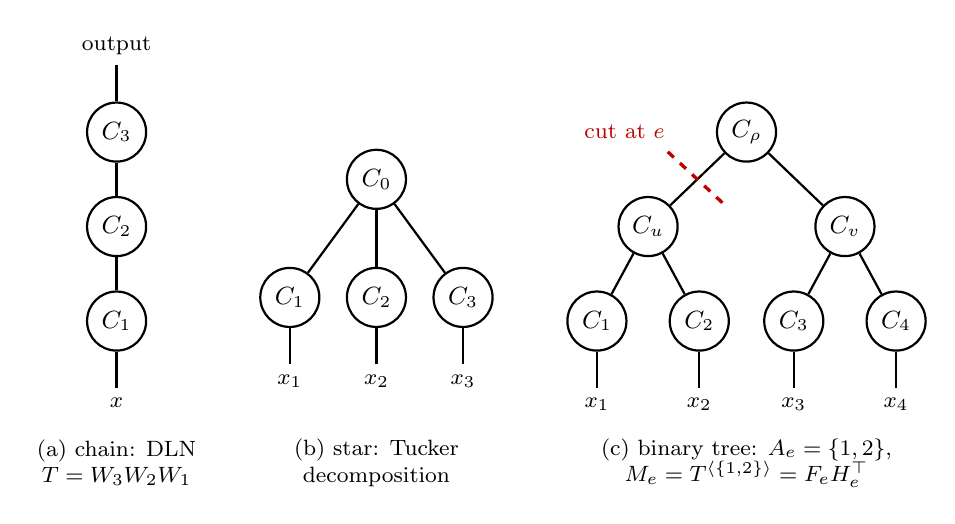
\begin{tikzpicture}[
  core/.style={circle, draw, thick, fill=white, minimum size=7.5mm, inner sep=0pt, font=\small},
  bond/.style={thick},
  leg/.style={thick},
  lab/.style={font=\footnotesize}]
  % (a) chain
  \node[core] (a1) at (0,0) {$C_1$};
  \node[core] (a2) at (0,1.2) {$C_2$};
  \node[core] (a3) at (0,2.4) {$C_3$};
  \draw[bond] (a1) -- (a2) (a2) -- (a3);
  \draw[leg] (a1) -- (0,-0.85) node[below, lab] {$x$};
  \draw[leg] (a3) -- (0,3.25) node[above, lab] {output};
  \node[lab, align=center] at (0,-1.8) {(a) chain: DLN\\$T=W_3W_2W_1$};
  % (b) star
  \begin{scope}[xshift=3.3cm]
    \node[core] (b0) at (0,1.8) {$C_0$};
    \foreach \i/\xx in {1/-1.1, 2/0, 3/1.1} {
      \node[core] (b\i) at (\xx,0.3) {$C_\i$};
      \draw[bond] (b0) -- (b\i);
      \draw[leg] (b\i) -- (\xx,-0.55) node[below, lab] {$x_\i$};
    }
    \node[lab, align=center] at (0,-1.8) {(b) star: Tucker\\decomposition};
  \end{scope}
  % (c) binary tree with a cut
  \begin{scope}[xshift=8.0cm]
    \node[core] (r) at (0,2.4) {$C_\rho$};
    \node[core] (u) at (-1.25,1.2) {$C_u$};
    \node[core] (v) at (1.25,1.2) {$C_v$};
    \foreach \i/\xx in {1/-1.9, 2/-0.6, 3/0.6, 4/1.9} {
      \node[core] (c\i) at (\xx,0) {$C_\i$};
      \draw[leg] (c\i) -- (\xx,-0.85) node[below, lab] {$x_\i$};
    }
    \draw[bond] (r) -- (u) (r) -- (v) (u) -- (c1) (u) -- (c2) (v) -- (c3) (v) -- (c4);
    \draw[red!75!black, dashed, very thick] (-1.0,2.15) -- (-0.25,1.45);
    \node[lab, red!75!black] at (-1.55,2.4) {cut at $e$};
    \node[lab, align=center] at (0,-1.8) {(c) binary tree: $A_e=\{1,2\}$,\\$M_e=T^{\langle\{1,2\}\rangle}=F_eH_e^\top$};
  \end{scope}
\end{tikzpicture}
\caption{Examples of tree tensor networks. Circles are cores, lines between circles are bonds, and dangling lines are open legs. (a) A chain is a deep linear network. (b) A star is a Tucker decomposition. (c) In a tree, cutting the bond $e$ splits the open legs into $A_e=\{1,2\}$ and its complement; the corresponding matricization factors through the bond, $M_e=F_eH_e^\top$ (Lemma~\ref{lem:cut}), so its rank is at most the bond dimension $D_e$.}
\label{fig:ttn}
\end{figure}

A TTN defines a model of functions once its legs receive inputs. If the input $x$ splits into blocks $(x^{(a)})_{a\in\Eext}$ and each leg receives a fixed embedding $\xi_a(x^{(a)})\in\R^{d_a}$ of its block (for example $\xi(z)=(1,z)$, or a one-hot encoding), the TTN computes
\begin{equation}\label{eq:ttn-model}
g_\vartheta(x)=\Big\langle T(\vartheta),\ \bigotimes_{a\in\Eext}\xi_a\big(x^{(a)}\big)\Big\rangle,
\end{equation}
which is multilinear in the embedded blocks and nonlinear in $x$ \citep{stoudenmire2016supervised}. We will meet two situations: \emph{physical} TTNs, whose legs receive distinct blocks of the input, and \emph{computational} TTNs, whose legs all receive copies of the same input (Section~\ref{sec:dpn}).

%----------------------------------------------------------------------
\subsection{Edge cuts, bond dimensions and hierarchical ranks}\label{sec:cuts}
%----------------------------------------------------------------------

The key structural property of a tree is that removing any edge disconnects it. Each bond therefore defines a bipartition of the open legs, hence a matricization of the represented tensor.

\begin{lemma}[Edge cuts]\label{lem:cut}
Let $T$ be the tensor represented by a TTN and let $e\in\Eint$. Removing $e$ splits the tree into two subtrees with vertex sets $V_e$ and $V_e^c$. Let $A_e\subseteq\Eext$ be the set of open legs attached to $V_e$, and $A_e^c=\Eext\setminus A_e$.
\begin{enumerate}[label=(\roman*),nosep]
\item $A_e$ and $A_e^c$ are nonempty, so $e$ defines the matricization $M_e:=T^{\langle A_e\rangle}\in\R^{m_e\times m_e^c}$, where $m_e=\prod_{a\in A_e}d_a$ and $m_e^c=\prod_{a\in A_e^c}d_a$.
\item $M_e=F_eH_e^\top$, where $F_e\in\R^{m_e\times D_e}$ (resp.\ $H_e\in\R^{m_e^c\times D_e}$) is the contraction of the cores in $V_e$ (resp.\ $V_e^c$) with the index of the bond $e$ left open.
\item $\rank M_e\le D_e$.
\end{enumerate}
\end{lemma}

\begin{proof}
(i) The subtree on $V_e$ is either a single vertex, which then has degree one in the tree, or it has at least two leaves, at most one of which is the endpoint of $e$. In both cases $V_e$ contains a leaf of the original tree, which carries an open leg. The same argument applies to $V_e^c$. (ii) Since $e$ is the only bond between $V_e$ and $V_e^c$, the sum~\eqref{eq:contraction} factorizes as a sum over $i_e\in[D_e]$ of the product of the contraction over $V_e$ and the contraction over $V_e^c$. (iii) follows from (ii).
\end{proof}

\begin{definition}[Bond dimension and hierarchical rank]\label{def:hrank}
The dimension $D_e$ of the index along which the two subtree matrices $F_e$ and $H_e$ are contracted is the \emph{bond dimension} of $e$. The family
\[
(M_e,\,r_e)_{e\in\Eint},\qquad r_e:=\rank M_e,
\]
collects the edge matricizations of $T$ and their ranks, and the tuple $r(T):=(r_e)_{e\in\Eint}$ is the \emph{hierarchical (Tucker) rank} of $T$ with respect to the tree. By Lemma~\ref{lem:cut}, $r_e\le D_e$: the rank across a cut is upper bounded by the bond dimension.
\end{definition}

The matrices $M_e$ and ranks $r_e$ depend only on the represented tensor $T$ and on which legs lie on each side of each bond, not on the cores. Cutting an open leg $a\in\Eext$ instead of a bond gives the mode matricization $T^{\langle\{a\}\rangle}$.

The bond dimensions describe exactly what a TTN can represent.

\begin{proposition}[Realizability; {\citealp{grasedyck2011introduction}}; {\citealp[Proposition~B.1]{furman2026benign}}]\label{prop:realizability}
Fix a tree with open legs. A tensor $T$ is represented by a TTN on this tree with bond dimensions $(D_e)_{e\in\Eint}$ if and only if $r_e(T)\le D_e$ for every $e\in\Eint$. In that case one can take $D_e=r_e(T)$.
\end{proposition}

\begin{proof}[Sketch]
Necessity is Lemma~\ref{lem:cut}(iii). For sufficiency, the column spaces of the matrices $M_e$ are nested along the tree (Proposition~\ref{prop:nested} below). Choosing a basis of each column space and expressing it in the bases of the children defines cores with $D_e=r_e$ that represent $T$ \citep[Proposition~B.1]{furman2026benign}; padding the cores with zeros gives any larger bond dimensions.
\end{proof}

Hence the model class of a TTN architecture is the set $\{T:\ r_e(T)\le D_e\ \forall e\in\Eint\}$. Since the set of matrices of rank at most $r$ is closed, this set is closed, and best approximations within it exist; this is not the case for the CP rank (Section~\ref{sec:ranks}).

\begin{remark}[Why trees: canonical matricizations]\label{rem:trees}
In a TTN, every bond $e$ determines exactly one bipartition $(A_e\mid A_e^c)$ of the open legs, and its bond dimension bounds the rank across that bipartition. The edge matricizations are therefore canonically attached to the network. This is not the case for tensor networks with cycles. There, removing a single edge does not disconnect the graph; a bipartition of the open legs is separated only by a set $C$ of edges, the rank across it is bounded by $\prod_{e\in C}D_e$, and a given edge belongs to the separating sets of many bipartitions. The correspondence between edges and matricizations is lost, and with it several properties used below: no characterization of the model class by ranks of matricizations such as Proposition~\ref{prop:realizability} is available in general, sets of tensors representable with bounded bond dimensions need not be closed \citep{landsberg2012geometry}, and canonical (minimum-norm) parameterizations are no longer unique up to gauge \citep[Remark~F.7]{furman2026benign}.
\end{remark}

The parameterization of a TTN is redundant: an invertible change of basis on a bond can be absorbed by the two adjacent cores.

\begin{proposition}[Gauge freedom]\label{prop:gauge}
Let $e=\{u,v\}\in\Eint$ and $X\in\GL(D_e)$. For a core $C$ incident to $e$, let $C\times_e X$ denote the core obtained by multiplying the mode of $C$ corresponding to $e$ by $X$, that is $(C\times_eX)_{\dots j\dots}=\sum_iC_{\dots i\dots}X_{ij}$. Replacing $C_u$ by $C_u\times_eX$ and $C_v$ by $C_v\times_eX^{-\top}$ leaves $T$ unchanged. Consequently the \emph{gauge group} $\mathcal G=\prod_{e\in\Eint}\GL(D_e)$ acts on the parameters and preserves $T$. Every quantity defined from $T$ alone, in particular $M_e$, $r_e$, and the singular values and singular subspaces of $M_e$, is gauge invariant, whereas individual core entries are not. If $D_e=r_e(T)$ for every $e$ (a minimal representation), then any two parameterizations of $T$ with these bond dimensions differ by a unique gauge transformation.
\end{proposition}

\begin{proof}
If $V_e$ contains $u$, the substitution maps $F_e$ to $F_eX$ and $H_e$ to $H_eX^{-\top}$, so $M_e=F_eH_e^\top$ is unchanged; since $M_e$ is a rearrangement of $T$, so is $T$. For the uniqueness statement for minimal representations see \citet{hackbusch2012tensor} and \citet{uschmajew2013geometry}.
\end{proof}

%----------------------------------------------------------------------
\subsection{The hierarchical singular value decomposition}\label{sec:hsvd}
%----------------------------------------------------------------------

Since every bond defines a canonical matricization, we can take its singular value decomposition.

\begin{definition}[SVD at a bond; hierarchical SVD]\label{def:hsvd}
For $e\in\Eint$, let
\[
M_e=U_eS_eV_e^\top
\]
be a compact SVD: $U_e\in\R^{m_e\times r_e}$ and $V_e\in\R^{m_e^c\times r_e}$ have orthonormal columns, and $S_e=\diag(\sigma_{e,1},\dots,\sigma_{e,r_e})$ with $\sigma_{e,1}\ge\cdots\ge\sigma_{e,r_e}>0$. Reshaping the $j$-th columns of $U_e$ and $V_e$ gives tensors $u_{e,j}$ over the legs in $A_e$ and $v_{e,j}$ over the legs in $A_e^c$, and, up to the order of the legs,
\begin{equation}\label{eq:schmidt-tensor}
T=\sum_{j=1}^{r_e}\sigma_{e,j}\;u_{e,j}\otimes v_{e,j}.
\end{equation}
The $\sigma_{e,j}$ are the \emph{hierarchical singular values} of $T$ at $e$, and $u_{e,j}$ (resp.\ $v_{e,j}$) its left (resp.\ right) singular vectors, which describe the subtree on one side of $e$ (resp.\ its environment). The \emph{hierarchical SVD} (HSVD) of $T$ is the family $(U_e,S_e,V_e)_{e\in\Eint}$ of the SVDs across all bonds of the TTN \citep{grasedyck2010hierarchical}.
\end{definition}

The HSVD is more than a list of unrelated SVDs: the singular vectors at different bonds are nested and fit together into a TTN.

\begin{proposition}[Nestedness; the HSVD is a TTN]\label{prop:nested}
Root the tree at a vertex $\rho$ and, for each bond $e$, let $A_e$ be the set of legs below $e$. Let $u\neq\rho$ be a vertex with parent bond $e$, child bonds $e_1,\dots,e_k$, and open legs of total dimension $n_u$ ($n_u=1$ if $u$ has no open leg). Then, after reordering the legs,
\begin{equation}\label{eq:nested}
\col(M_e)\subseteq\R^{n_u}\otimes\col(M_{e_1})\otimes\cdots\otimes\col(M_{e_k}).
\end{equation}
Consequently $B_u:=(I_{n_u}\otimes U_{e_1}\otimes\cdots\otimes U_{e_k})^\top U_e$ satisfies $U_e=(I_{n_u}\otimes U_{e_1}\otimes\cdots\otimes U_{e_k})\,B_u$. Set $B_\rho:=(I_{n_\rho}\otimes U_{e_1}\otimes\cdots\otimes U_{e_k})^\top\vect(T)$ at the root, where $e_1,\dots,e_k$ now denote the child bonds of $\rho$. The TTN with cores $(B_v)_{v\in V}$ and bond dimensions $(r_e)_{e\in\Eint}$ represents $T$, and in it the contraction of the subtree below each bond $e$ equals $U_e$; in particular $F_e=U_e$ has orthonormal columns.
\end{proposition}

\begin{proof}
Each column of $M_e$ is a partial contraction of $T$ against a fixed vector on the legs outside the subtree of $e$. Matricizing such a column with respect to the legs below a child bond $e_j$ gives columns that are partial contractions of $T$ against vectors on the legs outside the subtree of $e_j$, hence columns of $M_{e_j}$. A tensor whose matricizations along every child subtree have their columns in $\col(M_{e_j})$ lies in the right-hand side of~\eqref{eq:nested} \citep[proof of Proposition~B.1]{furman2026benign}. The identity for $U_e$ follows because $I\otimes U_{e_1}U_{e_1}^\top\otimes\cdots\otimes U_{e_k}U_{e_k}^\top$ is the orthogonal projector onto that right-hand side. The representation statement follows by induction from the leaves, the root step using~\eqref{eq:nested} for $T$ itself.
\end{proof}

\begin{remark}[Canonical and gauge invariant]\label{rem:hsvd-canonical}
The HSVD depends only on $T$ and on the tree, so it is gauge invariant (Proposition~\ref{prop:gauge}). It is unique up to the usual ambiguities of the SVD: the signs of singular vectors, and rotations within the eigenspaces of $M_eM_e^\top$ associated with repeated singular values. The singular values, and the singular subspaces of distinct singular values, are therefore canonical, and near a degeneracy one should compare whole singular subspaces rather than individual vectors. The orthonormal TTN of Proposition~\ref{prop:nested} is one canonical gauge. Another is the balanced, or minimum-norm, gauge of \citet[Appendix~F]{furman2026benign}, which is unique up to the orthogonal gauge group $\prod_e\mathrm O(D_e)$ and preserved by gradient flow; both carry the same gauge-invariant data.
\end{remark}

Truncating the HSVD gives a quasi-optimal compression.

\begin{proposition}[Truncation; {\citealp{grasedyck2010hierarchical}}]\label{prop:truncation}
Let $k_e\le r_e$ for $e\in\Eint$, and let $P_e$ be the orthogonal projector onto the span of the $k_e$ leading left singular vectors of $M_e$, acting on the legs in $A_e$. Enumerate the bonds $e_1,\dots,e_m$ so that every bond comes before the bonds below it. Then $T_k:=P_{e_m}\cdots P_{e_1}T$ satisfies $r_e(T_k)\le k_e$ for every $e$, and
\[
\norm{T-T_k}_F^2\ \le\ \sum_{e\in\Eint}\ \sum_{j>k_e}\sigma_{e,j}^2\ \le\ |\Eint|\cdot\min\big\{\norm{T-T'}_F^2:\ r_e(T')\le k_e\ \forall e\in\Eint\big\}.
\]
\end{proposition}

\begin{proof}
A projection at a bond below $e$, or in a subtree disjoint from the subtree below $e$, acts on one side of the cut at $e$ only, so it does not increase $r_e$; projections at bonds above $e$ are applied before $P_e$. For orthogonal projectors $\pi_1,\dots,\pi_m$, the decomposition $A-\pi_mB=(I-\pi_m)A+\pi_m(A-B)$ into orthogonal terms gives, by induction, $\norm{A-\pi_m\cdots\pi_1A}^2\le\sum_i\norm{(I-\pi_i)A}^2$, and $\norm{(I-P_e)T}_F^2=\sum_{j>k_e}\sigma_{e,j}^2$ by the Eckart--Young theorem \citep{eckart1936approximation}. Finally, for every $T'$ with $r_e(T')\le k_e$, Eckart--Young gives $\sum_{j>k_e}\sigma_{e,j}^2\le\norm{M_e-T'^{\langle A_e\rangle}}_F^2=\norm{T-T'}_F^2$. The minimum exists because the constraint set is closed.
\end{proof}

If two bonds define the same bipartition, as the two child bonds of a binary root do, projecting at one of them suffices; this gives the factor $2d-3$ of \citet{grasedyck2010hierarchical} for binary trees with $d$ leaves.

\begin{remark}[Stability]\label{rem:stability}
By Weyl's inequality, $|\sigma_{e,j}(T)-\sigma_{e,j}(T')|\le\norm{M_e(T)-M_e(T')}_{\mathrm{op}}\le\norm{T-T'}_F$: hierarchical singular values are 1-Lipschitz functions of the tensor. Singular subspaces are stable only relative to the gap that separates their singular values from the rest of the spectrum \citep{davis1970rotation,wedin1972perturbation}. These facts matter whenever the HSVDs of two models, or of one model at two times, are compared.
\end{remark}

%----------------------------------------------------------------------
\subsection{Notions of rank}\label{sec:ranks}
%----------------------------------------------------------------------

Tensors admit several notions of rank, which coincide for matrices but not for higher-order tensors \citep{kolda2009tensor,lim2021tensors}.

\begin{definition}[CP rank]
The \emph{CP rank} of $T$, $\rankcp(T)$, is the smallest number $R$ of rank-one tensors into which $T$ can be decomposed: $T=\sum_{s=1}^Ra_s^{(1)}\otimes\cdots\otimes a_s^{(n)}$ \citep{hitchcock1927expression}.
\end{definition}

The CP rank is challenging to compute in practice: deciding whether $\rankcp(T)\le R$ is NP-hard \citep{hastad1990tensor,hillar2013most}. Moreover, for $n\ge3$ and $R\ge2$ the set of tensors of CP rank at most $R$ is in general not closed, so a best approximation of low CP rank may fail to exist \citep{desilva2008tensor}.

\begin{definition}[Mode rank and Tucker rank]
The \emph{mode-$k$ rank} of $T$ is $r_k(T)=\rank T_{(k)}$, the rank of the matricization obtained by separating index $k$ from the others. The \emph{Tucker} (or multilinear) \emph{rank} is the tuple $(r_1(T),\dots,r_n(T))$ of all mode ranks. It is the smallest core size in a Tucker decomposition $T=\sum_{j_1,\dots,j_n}\Omega_{j_1\cdots j_n}\,u^{(1)}_{j_1}\otimes\cdots\otimes u^{(n)}_{j_n}$ \citep{tucker1966some,delathauwer2000multilinear}, i.e.\ a TTN on a star (Figure~\ref{fig:ttn}b).
\end{definition}

For a TTN, the \emph{hierarchical Tucker rank} is the tuple $(r_e)_{e\in\Eint}$ of Definition~\ref{def:hrank} \citep{hackbusch2009new,grasedyck2010hierarchical}. Mode ranks and hierarchical ranks are ranks of matrices: unlike the CP rank, they can be computed by SVDs, up to a numerical tolerance.

\begin{proposition}[Comparison of ranks]\label{prop:rank-comparison}
\leavevmode
\begin{enumerate}[label=(\roman*),nosep]
\item For every bipartition $A$, $\rank_A(T)\le\rankcp(T)$. In particular $r_k(T)\le\rankcp(T)$, and $r_e(T)\le\rankcp(T)$ for every tree.
\item In a rooted TTN, if a vertex $u$ has parent bond $e$, child bonds $e_1,\dots,e_k$ and open legs of total dimension $n_u$, then $r_e\le n_u\prod_{j=1}^kr_{e_j}$.
\item A tensor of CP rank $R$ is represented on every tree, with every assignment of legs to vertices, by a TTN whose bond dimensions all equal $R$ and whose cores are diagonal in the bond indices.
\end{enumerate}
\end{proposition}

\begin{proof}
(i) The $A$-matricization of a rank-one tensor has rank one, and the matrix rank is subadditive. (ii) Take dimensions in~\eqref{eq:nested}. (iii) Given $T=\sum_{s=1}^R\bigotimes_{a\in\Eext}w_s^{(a)}$, set $(C_v)_{(i_a)_{a},(j_e)_{e}}=\sum_{s=1}^R\prod_{e\ni v}\mathbf 1[j_e=s]\prod_{a}(w_s^{(a)})_{i_a}$, where $a$ ranges over the open legs at $v$ and $e$ over the bonds at $v$. Contracting forces all bond indices to agree, because the tree is connected \citep[Section~2.4]{hfl_diagonal}.
\end{proof}

The converse of (i) fails dramatically: TTNs with polynomially many parameters represent tensors whose CP rank is exponential in the number of leaves, for almost every choice of cores \citep{cohen2016expressive}. This is one precise sense in which hierarchical (deep) factorizations are more expressive than shallow ones.

\begin{remark}[Ranks and critical points]\label{rem:rank-critical}
\citet{furman2026benign} use a parameter-level notion: $\vartheta$ has \emph{full Tucker rank} if, for every bond $e$ and each of its endpoints $v$, the matricization of $C_v$ that separates the mode of $e$ has rank $D_e$. In general $r_e(T(\vartheta))$ is at most the ranks of these two matricizations, and equality holds at balanced (minimum-norm) parameters \citep[Proposition~D.2]{furman2026benign}. For a TTN with free cores trained on the Frobenius loss $\tfrac12\norm{T(\vartheta)-T^\star}_F^2$ (their setting, in which inputs are drawn uniformly among the entries of $T$, i.e.\ one-hot inputs) towards a realizable target $T^\star$, every critical point that is not a global minimum is rank deficient \citep[Theorem~5.2]{furman2026benign}; at such a point the network behaves as a TTN with smaller bond dimensions. For the parity of $n$ bits ($n\ge4$ a power of two), realized on a balanced binary tree with bond dimension $2$, the rank-one point whose cores all have entries $\tfrac12$, which is a best rank-one approximation, is a saddle of order at least $n/2$ \citep[Proposition~5.3]{furman2026benign}. Hierarchical ranks are therefore natural dynamical variables, and saddle-to-saddle dynamics should appear as successive increases of the rank profile. Whether these results extend to other losses, data distributions or constrained cores is open.
\end{remark}

%----------------------------------------------------------------------
\subsection{Deep polynomial networks as tree tensor networks}\label{sec:dpn}
%----------------------------------------------------------------------

We now show that deep networks with polynomial activations are TTNs with tied weights, evaluated on copies of the input.

\begin{definition}[Deep polynomial network]\label{def:dpn}
A feedforward network with $L$ hidden layers of widths $d_1,\dots,d_L$, acting on inputs $x\in\R^{d_0}$, is
\begin{equation}\label{eq:network}
h_0=x,\qquad z_\ell=W_\ell h_{\ell-1}+b_\ell,\qquad h_\ell=\sigma_\ell(z_\ell)\quad(1\le\ell\le L),\qquad f_\theta(x)=c^\top h_L+b_{\mathrm{out}},
\end{equation}
with $W_\ell\in\R^{d_\ell\times d_{\ell-1}}$, $b_\ell\in\R^{d_\ell}$, $c\in\R^{d_L}$ and $b_{\mathrm{out}}\in\R$ collected in $\theta$, and activations acting coordinatewise, $\sigma_\ell(z)_i=\sigma_{\ell,i}(z_i)$. It is a \emph{deep polynomial network} (DPN) if every $\sigma_{\ell,i}$ is a polynomial of degree at most $K$. It is a \emph{deep monomial network} (DMN) if moreover $\sigma_{\ell,i}(z)=z^K$ and all biases vanish ($b_\ell=0$, $b_{\mathrm{out}}=0$). A DMN with $K=2$ is a \emph{deep quadratic network} (DQN).
\end{definition}

Allowing the polynomial to depend on the neuron covers the Taylor surrogates of Section~\ref{sec:surrogate}. Since degrees multiply under composition, a DPN is a polynomial in $x$ of degree at most $K^L$.

\subsubsection{Monomial activations: tied TTNs on copies of the input}

\begin{proposition}[A monomial layer is one TTN vertex]\label{prop:monomial-layer}
Let $\sigma(z)=z^K$ and $W\in\R^{d'\times d}$. Then $\sigma(Wh)=A(h,\dots,h)$, where $A$ is the symmetric $K$-linear map
\[
A_{i\,j_1\cdots j_K}=\prod_{s=1}^KW_{ij_s},\qquad\text{i.e.}\qquad A(u_1,\dots,u_K)=(Wu_1)\odot\cdots\odot(Wu_K).
\]
In particular, for $K=2$,
\begin{equation}\label{eq:quadratic-layer}
\sigma(Wx)_i=\Big(\sum_jW_{ij}x_j\Big)^2=\sum_{j,k}W_{ij}x_j\,W_{ik}x_k=A(x,x)_i .
\end{equation}
\end{proposition}

The proof is the expansion of the product. Graphically,~\eqref{eq:quadratic-layer} is a vertex with one output leg $i$ and two input legs; equivalently, it is the Hadamard vertex $\Delta$ of Example~\ref{ex:bilinear} whose two input legs carry the same (tied) weight matrix $W$, applied to two copies of $x$. Composing layers gives a tree.

\begin{proposition}[DMNs are tied TTNs]\label{prop:dmn}
Let $f_\theta$ be a DMN with exponent $K\ge2$ and $L$ layers, and let $N=K^L$. Let $\mathcal T_{K,L}$ be the complete $K$-ary rooted tree of depth $L$ in which every non-root vertex at height $\ell$ carries the core $A_\ell$ of Proposition~\ref{prop:monomial-layer} built from $W_\ell$, the root (height $L$) carries the $K$-linear form $c^\top A_L$, and the vertices at height $1$ carry the $N$ open legs. Let $T(\theta)\in(\R^{d_0})^{\otimes N}$ be the represented tensor. Then
\[
f_\theta(x)=\big\langle T(\theta),\,x^{\otimes N}\big\rangle\qquad\text{for all }x\in\R^{d_0},
\]
and the bonds between heights $\ell$ and $\ell+1$ have dimension $d_\ell$.
\end{proposition}

\begin{proof}
Let $\Phi_\ell:(\R^{d_0})^{K^\ell}\to\R^{d_\ell}$ be the contraction of a subtree of height $\ell$: $\Phi_0=\mathrm{id}$ and $\Phi_\ell(y_1,\dots,y_{K^\ell})=A_\ell\big(\Phi_{\ell-1}(y^{(1)}),\dots,\Phi_{\ell-1}(y^{(K)})\big)$, where $y^{(s)}$ is the $s$-th block of $K^{\ell-1}$ consecutive arguments. Since $A_\ell(h,\dots,h)=\sigma(W_\ell h)$, induction gives $\Phi_\ell(x,\dots,x)=h_\ell(x)$, hence $f_\theta(x)=c^\top\Phi_L(x,\dots,x)=\ip{T(\theta)}{x^{\otimes N}}$.
\end{proof}

\begin{remark}[Copies, not copying]\label{rem:copies}
The map $x\mapsto x^{\otimes K}$ is not linear, so no tensor implements ``copying'' a vector. A DMN is therefore not a tensor network applied to $x$: it is the restriction of the $N$-linear map $T(\theta)$ to the diagonal $(x,\dots,x)$. The open legs are formal copies of the same input, and a cut of $\mathcal T_{K,L}$ separates copies, not input variables. The same identification, for networks with bilinear layers, is described as a TTN with a copying operation by \citet{pearce2024bilinear} and \citet{dooms2025compositionality} \citep[see][Section~2]{furman2026benign}.
\end{remark}

\begin{remark}[Hidden-unit symmetries are gauge transformations]\label{rem:symmetries}
Permuting the hidden units of layer $\ell$ by a permutation matrix $P$ ($W_\ell\mapsto PW_\ell$, $W_{\ell+1}\mapsto W_{\ell+1}P^\top$) does not change $f_\theta$, and neither does rescaling them, for monomial activations, by an invertible diagonal matrix $\Lambda$ ($W_\ell\mapsto\Lambda W_\ell$, $W_{\ell+1}\mapsto W_{\ell+1}\Lambda^{-K}$, with $c$ in place of $W_{L+1}$). On the tied TTN these symmetries act as gauge transformations, by $P$ and by $\Lambda^K$ respectively, on every bond of height $\ell$ (Proposition~\ref{prop:gauge}). Hence $T(\theta)$ and its HSVD are invariant under them, while the weights are not. This is the advantage of the TTN over the DMN parameterization: the HSVD gives a more canonical, gauge-independent description of internal structure. The idea is then to use the TTN representing a DMN to interpret its internal structure, reading the HSVD as the features that the network learns. Section~\ref{sec:features} makes this precise, and Remark~\ref{rem:which-tensor} discusses its limits.
\end{remark}

\subsubsection{General polynomial activations: homogenization}

Biases and lower-order terms break homogeneity. They are absorbed by adding a constant coordinate.

\begin{definition}[Homogenization]
Let $p(z)=\sum_{k=0}^Ka_kz^k$ be a polynomial of degree at most $K$. Its degree-$K$ \emph{homogenization} is
\[
p_h(z_0,z):=\sum_{k=0}^Ka_k\,z_0^{K-k}z^k,
\]
which equals $z_0^K\,p(z/z_0)$ for $z_0\neq0$. It is homogeneous of degree $K$, and $p_h(1,z)=p(z)$. The construction generalizes to multivariate polynomial maps: if $P:\R^n\to\R^m$ has degree at most $K$, $P(z)=\sum_{|\alpha|\le K}c_\alpha z^\alpha$ with $c_\alpha\in\R^m$, then $P_h(z_0,z)=\sum_{|\alpha|\le K}c_\alpha\,z_0^{K-|\alpha|}z^\alpha$ is a homogeneous polynomial map on $\R^{1+n}$ with $P_h(1,z)=P(z)$.
\end{definition}

A homogeneous polynomial can in turn be identified with a symmetric multilinear map.

\begin{lemma}[Polarization]\label{lem:polarization}
Let $Q:V\to W$ be a homogeneous polynomial map of degree $K$ between finite-dimensional real vector spaces. There is a unique symmetric $K$-linear map $S_Q:V^K\to W$ such that $S_Q(y,\dots,y)=Q(y)$ for all $y$, namely
\[
S_Q(y_1,\dots,y_K)=\frac1{K!}\sum_{\emptyset\neq J\subseteq[K]}(-1)^{K-|J|}\,Q\Big(\sum_{j\in J}y_j\Big).
\]
Conversely, every symmetric $K$-linear map $S$ defines the homogeneous polynomial $y\mapsto S(y,\dots,y)$.
\end{lemma}

This is the classical polarization identity. Combining the two steps, a polynomial of degree at most $K$ is a homogeneous polynomial of degree $K$ in one more variable, which is a symmetric $K$-linear map on the augmented space. For a polynomial activation, this map is a vertex with one output leg and $K$ input legs, which is why a DPN has a tree structure.

We write $H_\ell:=\R\oplus\R^{d_\ell}\cong\R^{1+d_\ell}$, with coordinates indexed from $0$, and $\hb:=(1,h)\in H_\ell$ for $h\in\R^{d_\ell}$.

\begin{proposition}[A polynomial layer is one TTN vertex; {\citealp[Section~3]{hfl_local}}]\label{prop:layer-core}
Let $P_\ell(h)=\sigma_\ell(W_\ell h+b_\ell)$ with polynomial activations $\sigma_{\ell,i}(z)=\sum_{s=0}^K\alpha_{\ell,i,s}(z-m_{\ell,i})^s$, for arbitrary expansion points $m_{\ell,i}$. Then $P_\ell(h)=\sum_{r=0}^KA_\ell^{(r)}[h^{\otimes r}]$, where $A_\ell^{(r)}:(\R^{d_{\ell-1}})^r\to\R^{d_\ell}$ is the symmetric $r$-linear map with components
\begin{equation}\label{eq:Ar}
A^{(r)}_{\ell;i}=\sum_{s=r}^K\binom{s}{r}\,\alpha_{\ell,i,s}\,q_{\ell,i}^{\,s-r}\;w_{\ell,i}^{\otimes r},\qquad q_{\ell,i}=b_{\ell,i}-m_{\ell,i},
\end{equation}
and $w_{\ell,i}^\top$ is the $i$-th row of $W_\ell$. Define $G_\ell:H_{\ell-1}^K\to H_\ell$ by, for $u_s=(a_s,v_s)\in\R\oplus\R^{d_{\ell-1}}$,
\begin{equation}\label{eq:G}
G_\ell(u_1,\dots,u_K)_0=\prod_{s=1}^Ka_s,\qquad
G_\ell(u_1,\dots,u_K)_{1:d_\ell}=\sum_{r=0}^K\binom{K}{r}^{-1}\sum_{\substack{S\subseteq[K]\\|S|=r}}A_\ell^{(r)}[v_s:s\in S]\prod_{s\notin S}a_s .
\end{equation}
Then $G_\ell$ is symmetric and $K$-linear, it is the polarization of the homogenized layer map, and
\begin{equation}\label{eq:diag-identity}
G_\ell(\hb,\dots,\hb)=\overline{P_\ell(h)}=\big(1,P_\ell(h)\big)\qquad\text{for all }h\in\R^{d_{\ell-1}}.
\end{equation}
In coordinates, an entry of $G_\ell$ with $r$ nonzero input indices equals the corresponding entry of $A_\ell^{(r)}$ divided by $\binom Kr$, and the only nonzero entry of the constant output slice is $(G_\ell)_{0;0\cdots0}=1$.
\end{proposition}

\begin{proof}
Equation~\eqref{eq:Ar} follows from the binomial expansion of $(w_{\ell,i}^\top h+q_{\ell,i})^s$. Each term of~\eqref{eq:G} is linear in each $u_s$, and permuting the $u_s$ permutes the subsets $S$, so $G_\ell$ is symmetric and $K$-linear. With $u_s=\hb$ for all $s$, the inner sum consists of $\binom Kr$ equal terms $A^{(r)}_\ell[h^{\otimes r}]$, which gives~\eqref{eq:diag-identity}. With $u_s=(a,v)$ for all $s$, $G_\ell$ returns $\big(a^K,\sum_ra^{K-r}A_\ell^{(r)}[v^{\otimes r}]\big)$, the homogenization of $h\mapsto(1,P_\ell(h))$; by Lemma~\ref{lem:polarization}, $G_\ell$ is its polarization.
\end{proof}

The factors $\binom Kr^{-1}$ prevent lower-order terms from being counted several times. Equation~\eqref{eq:Ar} also shows that the cores are constrained: all orders $r$ reuse the same weight row $w_{\ell,i}$, so $G_\ell$ is not a free tensor.

\begin{theorem}[Exact tied-TTN representation of a DPN; {\citealp[Proposition~1]{hfl_local}}; {\citealp[Proposition~1]{hfl_surrogate}}]\label{thm:dpn-ttn}
Let $f_\theta$ be a DPN with $L$ layers and activations of degree at most $K\ge2$, and let $N=K^L$. Consider the complete $K$-ary tree $\mathcal T_{K,L}$ in which every non-root vertex at height $\ell$ carries the core $G_\ell$ of Proposition~\ref{prop:layer-core}, the root carries the $K$-linear form $\cb^\top G_L$, i.e.\ its output is contracted with $\cb=(b_{\mathrm{out}},c)\in H_L$, and the $N$ open legs, attached to the vertices of height $1$, all receive the augmented input $\xb=(1,x)\in H_0$. Let $T(\theta)\in H_0^{\otimes N}$ be the represented tensor. Then
\begin{equation}\label{eq:dpn-ttn}
f_\theta(x)=\big\langle T(\theta),\,\xb^{\otimes N}\big\rangle\qquad\text{for all }x\in\R^{d_0}\text{ and all }\theta,
\end{equation}
and the bonds between heights $\ell$ and $\ell+1$ have dimension $d_\ell+1$. The map $\theta\mapsto T(\theta)$ is polynomial.
\end{theorem}

\begin{proof}
As in the proof of Proposition~\ref{prop:dmn}, let $\Phi_\ell:H_0^{K^\ell}\to H_\ell$ be the contraction of a subtree of height $\ell$: $\Phi_0=\mathrm{id}$ and $\Phi_\ell(y_1,\dots,y_{K^\ell})=G_\ell\big(\Phi_{\ell-1}(y^{(1)}),\dots,\Phi_{\ell-1}(y^{(K)})\big)$. By~\eqref{eq:diag-identity} and induction, $\Phi_\ell(\xb,\dots,\xb)=\hb_\ell(x)$. Hence $\ip{T(\theta)}{\xb^{\otimes N}}=\cb^\top\Phi_L(\xb,\dots,\xb)=b_{\mathrm{out}}+c^\top h_L(x)=f_\theta(x)$. The identity is algebraic, so it holds for every $\theta$.
\end{proof}

So a DPN is a weight-tied TTN applied to copies of the input $(1,x)$, the extra coordinate $1$ being induced by the homogenization; the bond dimension $d_\ell+1$ counts the hidden units of layer $\ell$ plus the constant. Figure~\ref{fig:quadratic} shows the case $K=L=2$. Since~\eqref{eq:dpn-ttn} holds identically in $\theta$, it can be differentiated: training the DPN in its own parameters is the same as training the tied TTN through the map $\theta\mapsto\big((G_\ell(\theta))_\ell,\cb\big)$ (Remark~\ref{rem:algebraic-dynamic}).

\begin{figure}[t]
\centering
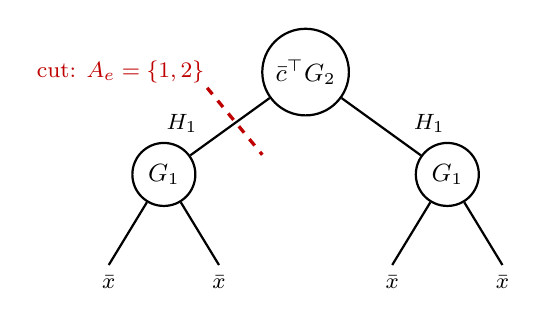
\begin{tikzpicture}[
  core/.style={circle, draw, thick, fill=white, minimum size=8mm, inner sep=0pt, font=\small},
  bond/.style={thick},
  leg/.style={thick},
  lab/.style={font=\footnotesize}]
  \node[core, minimum size=11mm] (g2) at (0,2.5) {$\bar c^{\top}G_2$};
  \node[core] (g1a) at (-1.8,1.2) {$G_1$};
  \node[core] (g1b) at (1.8,1.2) {$G_1$};
  \draw[bond] (g2) -- node[pos=0.78, above left, lab] {$H_1$} (g1a);
  \draw[bond] (g2) -- node[pos=0.78, above right, lab] {$H_1$} (g1b);
  \foreach \xx/\p in {-2.5/g1a, -1.1/g1a, 1.1/g1b, 2.5/g1b} {
    \draw[leg] (\p) -- (\xx,0.05) node[below, lab] {$\bar x$};
  }
  \draw[red!75!black, dashed, very thick] (-1.25,2.3) -- (-0.55,1.45);
  \node[lab, red!75!black] at (-2.35,2.5) {cut: $A_e=\{1,2\}$};
\end{tikzpicture}
\caption{The order-two surrogate of a network with two hidden layers, as a weight-tied binary TTN (Theorem~\ref{thm:dpn-ttn} and Example~\ref{ex:quadratic}, $K=L=2$). Both lower vertices carry the same core $G_1$; the $N=4$ open legs all receive the augmented input $\bar x=(1,x)\in H_0$; the bonds carry augmented hidden states $\bar h_1\in H_1=\R\oplus\R^{d_1}$; and the root carries $\bar c^\top G_2$, i.e.\ its output is contracted with $\bar c=(b_{\mathrm{out}},c)$. The cut shown defines $M_e$ with $A_e=\{1,2\}$; the other bond of height one gives the complementary bipartition and the same singular values (Proposition~\ref{prop:per-layer}).}
\label{fig:quadratic}
\end{figure}

\begin{remark}[What the representation is, and is not]\label{rem:qualifications}
\leavevmode
\begin{enumerate}[label=(\roman*),nosep]
\item It is a \emph{constrained} TTN: the cores are tied across each level, their entries satisfy the algebraic relations~\eqref{eq:Ar}, and the constant slice is fixed.
\item It is evaluated on the \emph{diagonal}: the leaves are formal copies of the whole input (Remark~\ref{rem:copies}).
\item The $N=K^L$ leaves are never materialized in computations: the recurrence~\eqref{eq:network} evaluates the same function at a cost linear in the depth, by sharing repeated subcomputations, i.e.\ as a circuit (a directed acyclic graph) rather than a tree.
\item For $K>2$, every $K$-ary vertex can be refined exactly into binary vertices, with new bond dimensions given by matricization ranks of $G_\ell$.
\item The multilinear extension is not unique. Since $\ip{T}{\xb^{\otimes N}}=\ip{\Sym T}{\xb^{\otimes N}}$, where $\Sym$ averages over permutations of the $N$ legs, $f_\theta$ determines only the symmetric part $\Sym T(\theta)$. It determines it uniquely: a homogeneous polynomial on $H_0$ is determined by its values on the hyperplane $\{y_0=1\}$, and a symmetric tensor by its homogeneous polynomial (Lemma~\ref{lem:polarization}). The tensor $T(\theta)$ is the particular extension induced by the architecture.
\end{enumerate}
\end{remark}

\begin{example}[Two layers, quadratic activations; {\citealp[Section~4]{hfl_local}}]\label{ex:quadratic}
For $K=2$, write each layer polynomial as $P_\ell(h)=a_\ell+A_\ell h+B_\ell(h,h)$ with $a_\ell\in\R^{d_\ell}$, $A_\ell$ linear and $B_\ell$ symmetric bilinear (these are $A_\ell^{(0)},A_\ell^{(1)},A_\ell^{(2)}$ in Proposition~\ref{prop:layer-core}). For the order-two Taylor polynomial of $\sigma_\ell$ at $m_\ell$ (Section~\ref{sec:surrogate}), with $\gamma^{(r)}_\ell=\sigma_\ell^{(r)}(m_\ell)$ taken coordinatewise and $q_\ell=b_\ell-m_\ell$,
\begin{gather*}
a_\ell=\gamma^{(0)}_\ell+\gamma^{(1)}_\ell\odot q_\ell+\tfrac12\gamma^{(2)}_\ell\odot q_\ell\odot q_\ell,\qquad
A_\ell u=\gamma^{(1)}_\ell\odot W_\ell u+\gamma^{(2)}_\ell\odot q_\ell\odot W_\ell u,\\
B_\ell(u,v)=\tfrac12\gamma^{(2)}_\ell\odot W_\ell u\odot W_\ell v .
\end{gather*}
The core~\eqref{eq:G} is $G_\ell\big((\alpha,u),(\beta,v)\big)=\big(\alpha\beta,\ a_\ell\,\alpha\beta+\tfrac12A_\ell(\alpha v+\beta u)+B_\ell(u,v)\big)$. For an output coordinate $i\ge1$, its matrix in the two input indices is
\[
(G_\ell)_{i;\,\cdot\,\cdot}=\begin{pmatrix}(a_\ell)_i&\tfrac12(A_\ell)_{i,:}\\[2pt]\tfrac12(A_\ell)_{i,:}^\top&(B_\ell)_{i;:,:}\end{pmatrix}.
\]
The network is $f_\theta(x)=\cb^\top G_2\big(G_1(\xb,\xb),G_1(\xb,\xb)\big)$, a polynomial of degree four (not two) in $x$, with coefficient tensor $T_{j_1j_2j_3j_4}=\sum_{r,a,b}\cb_r\,(G_2)_{r;ab}\,(G_1)_{a;j_1j_2}\,(G_1)_{b;j_3j_4}$. As a scalar check ($d_0=d_1=d_2=1$), for the SiLU activation $\sigma(z)=z/(1+e^{-z})$ with unit weights, zero biases, centres $0$ and unit readout, $p(z)=z/2+z^2/4$ and $f(x)=p(p(x))=x/4+3x^2/16+x^3/16+x^4/64$.
\end{example}

\subsubsection{Hierarchical features and learning capacity}\label{sec:features}

The representation allows us to define a notion of hierarchical features of a DPN, from the HSVD of its TTN, and a measure of learning capacity, from its hierarchical ranks. For the tied tree, the HSVD reduces to one SVD per layer.

\begin{proposition}[One SVD per layer]\label{prop:per-layer}
In the setting of Theorem~\ref{thm:dpn-ttn}, $T(\theta)$ is invariant under the permutations of its $N$ legs induced by automorphisms of $\mathcal T_{K,L}$. Consequently, for two bonds $e,e'$ at the same height, $M_{e'}$ is obtained from $M_e$ by permuting rows and columns: the two bonds have the same hierarchical singular values, and their singular vectors correspond under the relabelling of the leaves.
\end{proposition}

\begin{proof}
The cores $G_\ell$ and $\cb^\top G_L$ are symmetric in their $K$ inputs, so the contraction is invariant under exchanging the children of any vertex. These exchanges generate the automorphism group of $\mathcal T_{K,L}$, which acts transitively on the vertices of each height.
\end{proof}

We may therefore index the HSVD of a DPN by height: for $\ell=1,\dots,L-1$, it consists of singular values $\sigma_{\ell,1}\ge\cdots\ge\sigma_{\ell,r_\ell}>0$ and singular vectors $u_{\ell,j}\in H_0^{\otimes K^\ell}$, $v_{\ell,j}\in H_0^{\otimes(N-K^\ell)}$. (A network with one hidden layer has no bond; its cuts are mode matricizations.)

\begin{definition}[Hierarchical features]\label{def:features}
The \emph{hierarchical features} of the DPN $f_\theta$ at height $\ell$ are the pairs $(\sigma_{\ell,j},\varphi_{\ell,j})$, $j\le r_\ell$, where
\[
\varphi_{\ell,j}(x):=\big\langle u_{\ell,j},\,\xb^{\otimes K^\ell}\big\rangle
\]
is a polynomial of degree at most $K^\ell$. The complementary functions are $\psi_{\ell,j}(x):=\ip{v_{\ell,j}}{\xb^{\otimes(N-K^\ell)}}$.
\end{definition}

\begin{proposition}[What hierarchical features are]\label{prop:features}
For every $\ell\in\{1,\dots,L-1\}$:
\begin{enumerate}[label=(\roman*),nosep]
\item $f_\theta(x)=\sum_{j=1}^{r_\ell}\sigma_{\ell,j}\,\varphi_{\ell,j}(x)\,\psi_{\ell,j}(x)$ for all $x$;
\item there is a matrix $Q_\ell\in\R^{(d_\ell+1)\times r_\ell}$ such that $\varphi_{\ell,j}(x)=\sum_i(Q_\ell)_{ij}\,\hb_{\ell,i}(x)$: the hierarchical features at height $\ell$ are linear readouts of the augmented activations $\hb_\ell=(1,h_\ell)$ of layer $\ell$;
\item $r_\ell\le d_\ell+1$.
\end{enumerate}
\end{proposition}

\begin{proof}
(i) Contract~\eqref{eq:schmidt-tensor} with $\xb^{\otimes N}$. (ii) By Lemma~\ref{lem:cut}, $M_e=F_eH_e^\top$, so $\col(U_e)=\col(M_e)\subseteq\col(F_e)$, i.e.\ $U_e=F_eQ_\ell$ for some matrix $Q_\ell$. The $i$-th column of $F_e$ is the $i$-th coordinate of the subtree contraction $\Phi_\ell$, and $\Phi_\ell(\xb,\dots,\xb)=\hb_\ell(x)$ (proof of Theorem~\ref{thm:dpn-ttn}). (iii) is Lemma~\ref{lem:cut}(iii).
\end{proof}

The HSVD at height $\ell$ thus selects, among the directions of the activation space of layer $\ell$, those that the rest of the network uses, ranks them by $\sigma_{\ell,j}$, and is invariant under the hidden-unit symmetries of Remark~\ref{rem:symmetries}. Two cautions apply. The orthonormality of the $u_{\ell,j}$ refers to the Frobenius inner product of coefficient tensors, not to $L^2(\nu_x)$. And $\varphi_{\ell,j}$ and $\psi_{\ell,j}$ are functions of the same input, so (i) is not a decomposition of $f_\theta$ into functions of independent variables (Remark~\ref{rem:which-tensor}).

\begin{definition}[Learning capacity]\label{def:capacity}
The \emph{learning capacity} of a DPN at $\theta$ is the hierarchical rank profile of its TTN, $r(\theta)=(r_e(T(\theta)))_{e\in\Eint}$, that is $(r_\ell(\theta))_{\ell=1}^{L-1}$. It is bounded by the bond dimensions, $r_\ell\le D_\ell=d_\ell+1$, which form the maximal capacity of the architecture.
\end{definition}

By Proposition~\ref{prop:realizability}, a free TTN with bond dimensions $D$ represents exactly the tensors with $r\le D$, so $r(\theta)$ measures how much of the available capacity the model uses. Remark~\ref{rem:rank-critical} further suggests that learning proceeds by increasing ranks, although its results are proved for free TTNs on the Frobenius loss, not for the tied TTN of a DPN, whose loss depends on $T(\theta)$ only through $\Sym T(\theta)$ (Remark~\ref{rem:qualifications}(v)). A tuple of ranks raises a natural question.

\begin{question}[A global notion of learning capacity]\label{q:capacity}
What would be a reasonable global notion of learning capacity? The minimum, the sum, or the maximum of the ranks? Or some other complexity measure using the structure of the TTN?
\end{question}

\begin{remark}[Some candidates]\label{rem:capacity-candidates}
\leavevmode
\begin{enumerate}[label=(\alph*),nosep]
\item $\min_er_e$ and $\max_er_e$ measure the narrowest interface and the cost of contraction, respectively, but ignore where the ranks sit in the tree.
\item $\sum_e\log r_e$ is the logarithm of the product of the ranks; $\log r_e$ bounds the entropy of the normalized squared singular values $\sigma_{e,j}^2/\sum_i\sigma_{e,i}^2$ at $e$ (the entanglement entropy of quantum physics).
\item For a feasible profile $r$, the dimension of the set of tensors whose rank profile is exactly $r$,
\[
\dim(r)=\sum_{v\in V}n_v\prod_{e\ni v}r_e\;-\;\sum_{e\in\Eint}r_e^2,
\]
where $n_v$ is the product of the dimensions of the open legs at $v$, counts the parameters of a minimal TTN modulo the gauge group. It weights each rank by its position in the tree, and reduces to $r(m+n-r)$ for $m\times n$ matrices \citep{holtz2012manifolds,uschmajew2013geometry}.
\item Exact ranks are unstable, since a generic perturbation makes them maximal. Continuous surrogates, such as the participation ratio $(\sum_j\sigma_{e,j}^2)^2/\sum_j\sigma_{e,j}^4$ \citep[Section~9.4]{hfl_diagonal} or the entropy-based effective rank \citep{roy2007effective}, can be aggregated as in (a)--(c).
\end{enumerate}
Which of these, if any, predicts learning behaviour is an empirical question.
\end{remark}

\begin{remark}[Which tensor carries the features?]\label{rem:which-tensor}
Two caveats, emphasized by \citet[Section~8]{hfl_local} and \citet[Sections~3.4 and 7.4]{hfl_surrogate}, qualify the identification of the HSVD of $T(\theta)$ with the features learned by the network.

First, the HSVD of $T(\theta)$ is invariant under gauge transformations, hence under hidden-unit symmetries, but it is not an invariant of the function $f_\theta$. By Remark~\ref{rem:qualifications}(v), $f_\theta$ determines only $\Sym T(\theta)$, and different networks computing the same function can have different hierarchical ranks (Example~\ref{ex:same-function}). The HSVD is an invariant of the computation, not of the input--output map.

Second, cuts of the unrolled tree separate copies of the input, not input variables. When the input has independent blocks $x=(x_S,x_{S^c})$, with $\nu_x=\mu_S\otimes\mu_{S^c}$, an architecture-independent alternative is the functional SVD across a physical cut: every $g\in L^2(\nu_x)$ has a Schmidt decomposition
\[
g(x_S,x_{S^c})=\sum_{q\ge1}s_q(g)\,\phi^{S}_q(x_S)\,\phi^{S^c}_q(x_{S^c}),
\]
with $(\phi^S_q)_q$ orthonormal in $L^2(\mu_S)$ and $(\phi^{S^c}_q)_q$ orthonormal in $L^2(\mu_{S^c})$. Its singular values and subspaces depend only on $g$ and $\nu_x$, so they can be compared between a teacher, a DNN, its polynomial surrogate and any TTN. Organizing such cuts along a tree of input blocks gives a physical-block TTN and HSVD, whose ranks are not bounded by the widths $d_\ell$. In practice, they can be estimated from the crossed-grid matrix $\big[g(u_a,v_b)/\sqrt{n_Ln_R}\big]_{a\le n_L,\,b\le n_R}$ built from independent samples $u_a\sim\mu_S$ and $v_b\sim\mu_{S^c}$ \citep[Section~8.4]{hfl_local}. The computational HSVD of Definition~\ref{def:features} and the physical one answer different questions: the first describes how the network computes, the second what it computes.
\end{remark}

\begin{example}[Same function, different hierarchical ranks]\label{ex:same-function}
Take $d_0=2$ and two DQNs with two layers (Definition~\ref{def:dpn}, $K=L=2$) computing $f(x)=x_1^2x_2^2$. Network P has $W_1=\left(\begin{smallmatrix}1&1\\1&-1\end{smallmatrix}\right)$, so that $h_1=\big((x_1+x_2)^2,(x_1-x_2)^2\big)$, then $W_2=(\tfrac14,-\tfrac14)$ and $c=1$, so that $z_2=x_1x_2$ and $f=z_2^2$. Network Q has $W_1=I_2$, so that $h_1=(x_1^2,x_2^2)$, then $W_2=\left(\begin{smallmatrix}1&1\\1&-1\end{smallmatrix}\right)$ and $c=(\tfrac14,-\tfrac14)$. With the bilinear forms $Z(u,v)=\tfrac12(u_1v_2+u_2v_1)$, $Z_a(u,v)=u_1v_1$ and $Z_b(u,v)=u_2v_2$, Proposition~\ref{prop:dmn} gives
\begin{align*}
T_P(y_1,y_2,y_3,y_4)&=Z(y_1,y_2)\,Z(y_3,y_4),\\
T_Q(y_1,y_2,y_3,y_4)&=\tfrac12\big[Z_a(y_1,y_2)Z_b(y_3,y_4)+Z_b(y_1,y_2)Z_a(y_3,y_4)\big].
\end{align*}
Both restrict to $x_1^2x_2^2$ on the diagonal, but the hierarchical rank of the bond at height one is $r_1=1$ for P and $r_1=2$ for Q. By contrast, for independent inputs $x_1$ and $x_2$, the functional rank of $f$ across the physical cut $x_1\mid x_2$ is $1$, whichever network computes it.
\end{example}

\begin{question}[Interpretability]\label{q:interpretability}
If we use the TTN as a surrogate model and its HSVD to interpret it, do the hierarchical singular values and vectors correspond to some meaningful structure? For example, if we use a toy model that we can interpret, do the features of the TTN correspond to the known features? Modular arithmetic would be an interesting example to investigate.
\end{question}

The following computation shows what to expect in the modular arithmetic case, in which the mechanism learned by small networks is known.

\begin{example}[Modular addition]\label{ex:modular}
Let $p$ be an odd prime, encode inputs $a,b\in\mathbb Z_p$ as one-hot vectors, and let a model output logits $o(a,b)\in\R^p$, as in the grokking setting of \citet{power2022grokking}. Since every function of $(a,b)$ is bilinear in the one-hot encodings, the model is exactly a tensor $L\in\R^{p\times p\times p}$, $L_{abc}=o(a,b)_c$: a TTN on the physical tree with leaves $a$, $b$ and output $c$. Its HSVD across the cut that separates $a$ is the SVD of $L^{\langle\{a\}\rangle}\in\R^{p\times p^2}$. This is a function-level (physical) HSVD: it depends only on the logits, not on the architecture that computes them (Remark~\ref{rem:which-tensor}).
\begin{enumerate}[label=(\roman*),nosep]
\item The target $T^\star_{abc}=\mathbf 1[c\equiv a+b]$ has a maximally degenerate spectrum. The rows of $T^{\star\langle\{a\}\rangle}$ are orthogonal and each contains $p$ ones, so $T^{\star\langle\{a\}\rangle}\big(T^{\star\langle\{a\}\rangle}\big)^\top=p\,I_p$ and all $p$ singular values equal $\sqrt p$. The SVD alone therefore singles out no basis, in particular not the Fourier basis. The same holds for the two other cuts.
\item \citet{nanda2023progress} found that one-layer transformers trained on modular addition implement a Fourier algorithm whose logits are approximately $L_{abc}=\sum_{k\in\mathcal F}\lambda_k\cos\big(2\pi k(a+b-c)/p\big)$, for a small set $\mathcal F\subseteq\{1,\dots,(p-1)/2\}$ of key frequencies. If the $\lambda_k>0$ are distinct, then $L^{\langle\{a\}\rangle}$ has rank $2|\mathcal F|$ and singular values $\lambda_kp^{3/2}/2$, each with multiplicity two, and the corresponding left singular subspaces are $\mathrm{span}\{(\cos(2\pi ka/p))_{a},(\sin(2\pi ka/p))_{a}\}$. Indeed, with $\omega_k=2\pi k/p$,
\[
\cos\big(\omega_k(a+b-c)\big)=\cos(\omega_ka)\cos\big(\omega_k(b-c)\big)-\sin(\omega_ka)\sin\big(\omega_k(b-c)\big),
\]
and these vectors are mutually orthogonal across $k$ and between $\cos$ and $\sin$, with squared norms $p/2$ as functions of $a$ and $p^2/2$ as functions of $(b,c)$.
\end{enumerate}
For this idealized mechanism, the physical HSVD thus recovers exactly the known features, as two-dimensional frequency subspaces ranked by their strengths $\lambda_k$; the rotation within each subspace reflects the translation symmetry of $\mathbb Z_p$. Question~\ref{q:interpretability} asks more: whether the HSVD of the computational TTN of a trained network (Section~\ref{sec:features}), which describes how the network computes, also recovers these subspaces. A natural test case is an MLP with quadratic activations acting on the concatenated one-hot inputs, for which an analytic Fourier solution is known in the case of one hidden layer \citep{gromov2023grokking}. With one hidden layer, the computational cuts are the mode matricizations of the root core; with more layers, Definition~\ref{def:features} applies.
\end{example}

%----------------------------------------------------------------------
\subsection{Surrogate model of a deep neural network}\label{sec:surrogate}
%----------------------------------------------------------------------

Consider a general DNN~\eqref{eq:network} with smooth activation functions, more precisely of class $C^{k+1}$ on intervals that contain all the pre-activations of the network and of its surrogate. The idea is to Taylor expand the DNN into a DPN around a training checkpoint, and to represent this DPN as a TTN.

\begin{definition}[Layerwise Taylor surrogate; {\citealp[Section~2.2]{hfl_local}}]\label{def:taylor-surrogate}
Let $\theta_j=\theta(t_j)$ be a checkpoint, $\mathcal C$ a finite calibration set of inputs, and $k\ge1$. For every layer $\ell$ and neuron $i$, let the \emph{centre}
\[
m_{\ell,j,i}:=\frac1{|\mathcal C|}\sum_{x\in\mathcal C}z_{\ell,i}(\theta_j,x)
\]
be the average pre-activation of the neuron over the calibration set at the checkpoint, and let
\[
p^{(k)}_{\ell,j,i}(z):=\sum_{r=0}^k\frac{\sigma_{\ell,i}^{(r)}(m_{\ell,j,i})}{r!}\,(z-m_{\ell,j,i})^r
\]
be the order-$k$ Taylor polynomial of $\sigma_{\ell,i}$ at that centre. The \emph{order-$k$ surrogate at checkpoint $j$} is the DPN obtained by replacing every activation by its Taylor polynomial, while using the surrogate's own hidden states:
\[
\hat h_0=x,\qquad\hat z_\ell=W_\ell\hat h_{\ell-1}+b_\ell,\qquad\hat h_\ell=p^{(k)}_{\ell,j}(\hat z_\ell),\qquad\fhat_j(\theta,x)=c^\top\hat h_L+b_{\mathrm{out}}.
\]
The centres and the Taylor coefficients are frozen, and $\theta$ remains trainable.
\end{definition}

\begin{definition}[TTN surrogate]\label{def:ttn-surrogate}
For $k\ge2$, the \emph{TTN surrogate} of the DNN at checkpoint $j$ is the tied TTN of Theorem~\ref{thm:dpn-ttn}, with $K=k$, that represents the surrogate: $\fhat_j(\theta,x)=\ip{T_j(\theta)}{\xb^{\otimes k^L}}$. We say that this TTN is a surrogate model of the DNN at the training point $\theta_j$.
\end{definition}

\begin{remark}[On the definition]\label{rem:surrogate-def}
\leavevmode
\begin{enumerate}[label=(\roman*),nosep]
\item The surrogate must use its own hidden states: substituting the true hidden states of the DNN at every layer would define an error diagnostic, not a trainable model.
\item Its input degree is $k^L$, not $k$. Layerwise Taylorization is not the Taylor expansion of the predictor in $\theta$ \citep{bai2020taylorized}, since composition keeps cross-layer terms of all orders. For $k=1$, every activation is replaced by its tangent line and the surrogate is a deep affine network, i.e.\ a DLN with biases, not the linearized (NTK) model; its TTN degenerates into a chain. The family of surrogates therefore starts from the model whose dynamics is understood.
\item The centre lives in pre-activation space, since $\sigma$ is expanded in its argument. Expanding around the mean pre-activation over a calibration set places the expansion at a typical value over the input distribution; the mean minimizes the mean squared distance to the centre, which controls the order-one remainder, but it is a heuristic and not an optimal choice in general.
\item Choosing instead the per-example centre $m_{\ell,j}(x)=z_\ell(\theta_j,x)$ makes the surrogate agree with the DNN and its $\theta$-derivatives up to order $k$ at $\theta_j$, so that $\fhat_j(\theta_j+\Delta,\cdot)-f_{\theta_j+\Delta}=O(\norm\Delta^{k+1})$ under suitable bounds. Its coefficients, however, depend on $x$, so it is not one polynomial in $x$ and has no single TTN. It is a useful control, which separates the error due to the spread of pre-activations across inputs from the error due to training \citep[Section~2.3]{hfl_local}.
\item Layerwise Taylorization of trained networks also underlies NN2Poly \citep{morala2025nn2poly}; for higher-order dynamical approximations in parameter space, see \citet{bai2020taylorized} and \citet{huang2020dynamics}.
\item In automatic differentiation, the centres and the derivatives $\sigma^{(r)}(m)$ must be detached from the computational graph, while the cores $G_\ell$, recomputed from the current $\theta$, must remain differentiable.
\end{enumerate}
\end{remark}

We would like to know how good an approximation of the DNN such a TTN is. Since training follows gradients, the relevant errors are on derivatives as well as values.

\begin{lemma}[Taylor remainders]\label{lem:taylor}
If $\sigma$ is $C^{k+1}$ on the segment between $m$ and $z$, and $M_{k+1}$ bounds $|\sigma^{(k+1)}|$ there, then
\[
\big|\sigma(z)-p^{(k)}(z)\big|\le\frac{M_{k+1}}{(k+1)!}\,|z-m|^{k+1},\qquad
\big|\sigma'(z)-(p^{(k)})'(z)\big|\le\frac{M_{k+1}}{k!}\,|z-m|^{k}.
\]
\end{lemma}

\begin{proof}
Use the Lagrange form of the remainder; for the second inequality, note that $(p^{(k)})'$ is the order-$(k-1)$ Taylor polynomial of $\sigma'$ at $m$.
\end{proof}

\begin{proposition}[Loss-gradient defect; {\citealp[Proposition~2]{hfl_local}}]\label{prop:defect}
Let $\mathcal L(\theta)=\frac12\E_\nu[(f_\theta(x)-y)^2]$ and $\Lhat_j(\theta)=\frac12\E_\nu[(\fhat_j(\theta,x)-y)^2]$, and define at a common parameter $\theta$
\begin{align*}
\varepsilon_{0,j}&=\norm{f_\theta-\fhat_j(\theta,\cdot)}_{L^2(\nu_x)}, &
\varepsilon_{1,j}&=\norm{\nabla_\theta f_\theta-\nabla_\theta\fhat_j(\theta,\cdot)}_{L^2(\nu_x)},\\
R_y&=\norm{f_\theta-y}_{L^2(\nu)}, &
B_j&=\norm{\nabla_\theta\fhat_j(\theta,\cdot)}_{L^2(\nu_x)},
\end{align*}
where $\norm{v}_{L^2}=\E[\norm{v}^2]^{1/2}$ for vector-valued $v$. Whenever differentiation under the expectation is valid,
\[
\norm{\nabla\mathcal L(\theta)-\nabla\Lhat_j(\theta)}\le R_y\,\varepsilon_{1,j}+B_j\,\varepsilon_{0,j}=:\beta_j(\theta).
\]
\end{proposition}

\begin{proof}
$\nabla\mathcal L-\nabla\Lhat_j=\E\big[(f-y)(\nabla f-\nabla\fhat_j)+(f-\fhat_j)\nabla\fhat_j\big]$; apply the triangle and Cauchy--Schwarz inequalities.
\end{proof}

Two functions can thus be close while their parameter derivatives, and therefore their training updates, are different: prediction agreement alone is not sufficient.

\begin{proposition}[Trajectory comparison; {\citealp[Section~6]{hfl_local}}]\label{prop:gronwall}
Let $\theta$ and $\tilde\theta$ solve $\dot\theta=-\nabla\mathcal L(\theta)$ and $\dot{\tilde\theta}=-\nabla\Lhat_j(\tilde\theta)$ on $[t_j,t_j+h]$, and assume that both stay in a set $\mathcal U$ on which $\nabla\mathcal L$ is $\kappa_j$-Lipschitz and $\norm{\nabla\mathcal L-\nabla\Lhat_j}\le\beta_j$. Then $E(s):=\norm{\theta(t_j+s)-\tilde\theta(t_j+s)}$ satisfies
\[
E(s)\le e^{\kappa_js}E(0)+\beta_j\,\frac{e^{\kappa_js}-1}{\kappa_j},\qquad0\le s\le h,
\]
the fraction being $s$ if $\kappa_j=0$. For gradient descent with steps $\eta_n$, $E_{n+1}\le(1+\eta_n\kappa_j)E_n+\eta_n\beta_j$.
\end{proposition}

\begin{proof}
The upper Dini derivative satisfies $D^+E\le\norm{\nabla\mathcal L(\theta)-\nabla\mathcal L(\tilde\theta)}+\norm{\nabla\mathcal L(\tilde\theta)-\nabla\Lhat_j(\tilde\theta)}\le\kappa_jE+\beta_j$; integrate (Gr\"onwall). The discrete case is identical.
\end{proof}

These statements make the quality of the approximation precise: the local surrogate is faithful over windows on which the loss-gradient defect $\beta_j$ is small compared with the gradient itself. They are conditional, and their constants can grow with depth, width and parameter norms; \citet[Appendix~A]{hfl_local} propagates the remainders of Lemma~\ref{lem:taylor} through the layers into $\varepsilon_{0,j}$ and $\varepsilon_{1,j}$.

\begin{remark}[Fixed centres have an error floor]\label{rem:floor}
With input-independent centres, the radius $|z-m|$ in Lemma~\ref{lem:taylor} includes the spread $S_{\ell,j}=\sup_x\norm{z_\ell(\theta_j,x)-m_{\ell,j}}_\infty$ of the pre-activations around the centres, which does not shrink with the time window \citep[Section~6.3]{hfl_local}. The gradient defect $\norm{\nabla\mathcal L(\theta_j)-\nabla\Lhat_j(\theta_j)}$ at the checkpoint is then generally nonzero, and since both trajectories start at $\theta_j$, $E(s)=s\,\norm{\nabla\mathcal L(\theta_j)-\nabla\Lhat_j(\theta_j)}+o(s)$: the error grows linearly from the start of the window, and Proposition~\ref{prop:gronwall} gives a matching upper bound. If the fixed-centre surrogate fails while the per-example surrogate of Remark~\ref{rem:surrogate-def}(iv) succeeds, the problem is the spread of activations across inputs, not the tensor representation. Chebyshev or distribution-weighted polynomial fits over the observed range of pre-activations are then natural, non-Taylor alternatives \citep[Section~8.2]{hfl_surrogate}.
\end{remark}

We would also like to know whether the HSVD of the TTN can be used to extract the structure that the DPN has learned, and to predict its training dynamics. The following identity connects the two.

\begin{proposition}[Dynamics of hierarchical singular values]\label{prop:sv-dynamics}
Let $N=k^L$. Along the gradient flow $\dot\theta=-\nabla\Lhat_j(\theta)$ of the surrogate, the tensor $T(t):=T_j(\theta(t))$ evolves as
\[
\dot T=-\mathcal K_\theta\big[R_\theta\big],\qquad
\mathcal K_\theta:=DT_j(\theta)\,DT_j(\theta)^*,\qquad
R_\theta:=\E_\nu\big[(\fhat_j(\theta,x)-y)\,\xb^{\otimes N}\big],
\]
where $\mathcal K_\theta$ is a positive semidefinite operator on $H_0^{\otimes N}$ and $R_\theta$ is the residual-weighted moment tensor. If $\sigma_{e,i}$ is a simple nonzero singular value of $M_e(t)$, then it is differentiable and
\[
\dot\sigma_{e,i}=u_{e,i}^\top\dot M_e\,v_{e,i}=-\big\langle Y_{e,i},\,\mathcal K_\theta[R_\theta]\big\rangle,
\]
where $Y_{e,i}$ is the tensor whose $A_e$-matricization is $u_{e,i}v_{e,i}^\top$.
\end{proposition}

\begin{proof}
We have $\Lhat_j=\mathcal J\circ T_j$ with $\mathcal J(T)=\frac12\E_\nu[(\ip{T}{\xb^{\otimes N}}-y)^2]$, whose gradient is $R$. By the chain rule, $\dot\theta=-DT_j(\theta)^*[R_\theta]$ and $\dot T=DT_j(\theta)[\dot\theta]$. For a simple singular value with unit singular vectors, $\sigma=u^\top Mv$ and $\dot\sigma=u^\top\dot Mv+\sigma(\dot u^\top u+v^\top\dot v)=u^\top\dot Mv$, because $\norm u=\norm v=1$.
\end{proof}

The identity is exact but not closed: $\mathcal K_\theta$, $R_\theta$ and the singular vectors all evolve. Predicting the training dynamics from the HSVD amounts to finding regimes in which a few singular values and subspaces approximately close under these equations \citep[Section~12]{hfl_surrogate}, as the singular modes of a DLN do in the analysis of \citet{saxe2014exact}. When surrogates built at different checkpoints are compared, their HSVDs should be evaluated at the same parameter value, since otherwise a change of Taylor centres would be mistaken for learning (\citealp[Section~8.5]{hfl_local}; \citealp[Section~9.1]{hfl_surrogate}); Remark~\ref{rem:stability} bounds how much the spectrum can move.

\paragraph{A more direct approach: polynomial activations.}
Another, more direct approach is to replace the activation functions of the original network by polynomial activation functions. We then train the corresponding TTN, define some useful observables, such as the HSVD, and check whether their training dynamics is similar to that of the original DNN.

\begin{definition}[Polynomial-activation proxy]\label{def:poly-proxy}
Given the architecture~\eqref{eq:network} with activation $\sigma$, choose polynomials $q_\ell$ of degree $K$, for example the Taylor polynomial of $\sigma$ at a fixed point, or a least-squares fit of $\sigma$ on an interval $[-a,a]$ that contains most pre-activations. The \emph{polynomial proxy} $f^q_\theta$ is the DPN obtained by replacing $\sigma_\ell$ with $q_\ell$, initialized and trained exactly like the DNN. By Theorem~\ref{thm:dpn-ttn}, $f^q_\theta(x)=\ip{T^q(\theta)}{\xb^{\otimes K^L}}$, so the hierarchical singular values $\sigma_{\ell,j}(t)$ and ranks $r_\ell(t)$ of Definitions~\ref{def:features} and~\ref{def:capacity} can be tracked along its training. They are diagnostics of the TTN representation; they can be compared with the DNN through the HSVDs of its local TTN surrogates (Definition~\ref{def:ttn-surrogate}), or through physical HSVDs (Remark~\ref{rem:which-tensor}).
\end{definition}

\begin{remark}[Algebraic equivalence is not dynamical equivalence]\label{rem:algebraic-dynamic}
``Training the corresponding TTN'' can mean two different things. (a) Training the DPN in its parameters $\theta$ is identical to training the tied TTN through the map $\Gamma:\theta\mapsto\big((G_\ell(\theta))_\ell,\cb\big)$, because~\eqref{eq:dpn-ttn} holds identically in $\theta$. (b) Training the cores $g$ as free variables is a different dynamical system: if $g=\Gamma(\theta)$ and $\mathcal J(g)$ denotes the loss as a function of the cores, (a) induces $\dot g=-D\Gamma(\theta)D\Gamma(\theta)^\top\nabla_g\mathcal J(g)$, a preconditioned and possibly degenerate flow, whereas (b) is $\dot g=-\nabla_g\mathcal J(g)$. Moreover, free training breaks the ties and constraints of Remark~\ref{rem:qualifications}(i). \citet[Section~4.1]{hfl_surrogate} proposes a ladder of relaxations that isolates each simplification: the tied TTN trained through $\theta$; free tied cores with the induced metric; a block-diagonal approximation of that metric; Euclidean core gradients; untied cores; compressed ranks; and finally a different tree. For computations, one should use the recurrence~\eqref{eq:network} rather than the exponentially large tree.
\end{remark}

\begin{remark}[Choosing the degree]\label{rem:degree}
A problem is to choose the degree of the nodes of the TTN. Several considerations bear on it.
\begin{enumerate}[label=(\roman*),nosep]
\item Approximation: on a bounded range of pre-activations, least-squares or Chebyshev approximations of a smooth activation improve rapidly with $K$, whereas Taylor polynomials are accurate only near their centre.
\item Stability: polynomials are unbounded and the degree $K^L$ of the network grows exponentially with depth, so pre-activations that leave the fitted range are amplified. The fraction of pre-activations outside that range is a direct diagnostic \citep[Section~8.8]{hfl_surrogate}.
\item Structure: $K=2$ is the smallest nonlinear choice and gives binary trees. Networks with bilinear layers $(Wx)\odot(Vx)$, which are untied versions of quadratic activations, are competitive in practice and can be interpreted through their tensors \citep{pearce2024bilinear}.
\item Cost: each core has order $K+1$, while the bond dimensions $d_\ell+1$ do not depend on $K$.
\end{enumerate}
A pragmatic rule is to choose the smallest $K$ for which the defects of Proposition~\ref{prop:defect} are below a tolerance at initialization and at a few checkpoints.
\end{remark}
\section{Training dynamics of TTNs}

%======================================================================
\section{How to compare TTNs and DNNs}\label{sec:compare}
%======================================================================

We want to test experimentally whether the training dynamics of TTNs is similar to that of DNNs with standard activation functions, such as ReLU, GELU or SiLU. Hypothesis~\ref{hyp:global} phrases this question in terms of observables, i.e.\ quantities that can be evaluated along the trajectory of any architecture. This section constructs such observables in the setting in which they are easiest to interpret: a teacher--student experiment in which the teacher is a TTN. The teacher's tree then provides a canonical hierarchy of interfaces, its bonds, and the singular value decomposition across each bond provides a canonical, gauge-invariant list of candidate features, which we call \emph{atoms}. Comparing a TTN with a DNN then amounts to asking, for each atom and each student, when the student acquires the atom, where it computes it, and whether it relies on it.

These questions call for different kinds of evidence, which should not be conflated (Figure~\ref{fig:compare}):
\begin{enumerate}[label=(\roman*),nosep]
\item \emph{output}: the predictor of the student contains the atom, with the teacher's strength;
\item \emph{representation}: the atom, or the two factors of which it is the product, can be read off a hidden layer of the student;
\item \emph{use}: the computation downstream of that layer is sensitive to this internal code, and causally relies on it.
\end{enumerate}
Section~\ref{sec:compare-setting} fixes the setting, and Sections~\ref{sec:dw-hsvd} and~\ref{sec:atoms} define the atoms of the teacher. The HSVD of Section~\ref{sec:hsvd} has to be modified for this purpose, because it is computed in the Euclidean geometry of coefficient tensors, whereas learning takes place in the geometry of the data. Section~\ref{sec:output-obs} defines output observables in the coordinates of the teacher, and Section~\ref{sec:student-fsvd} complements them with a teacher-free description of a student, its own functional SVD. Sections~\ref{sec:representation} and~\ref{sec:use} define the representation and use observables. Section~\ref{sec:ttn-students} explains why all observables are simpler, and partly exact, for TTN students. Section~\ref{sec:compare-protocol} turns the observables into acquisition times, comparisons between students and an estimation protocol, and Table~\ref{tab:evidence} in Section~\ref{sec:compare-summary} summarizes them.

\begin{figure}[t]
\centering
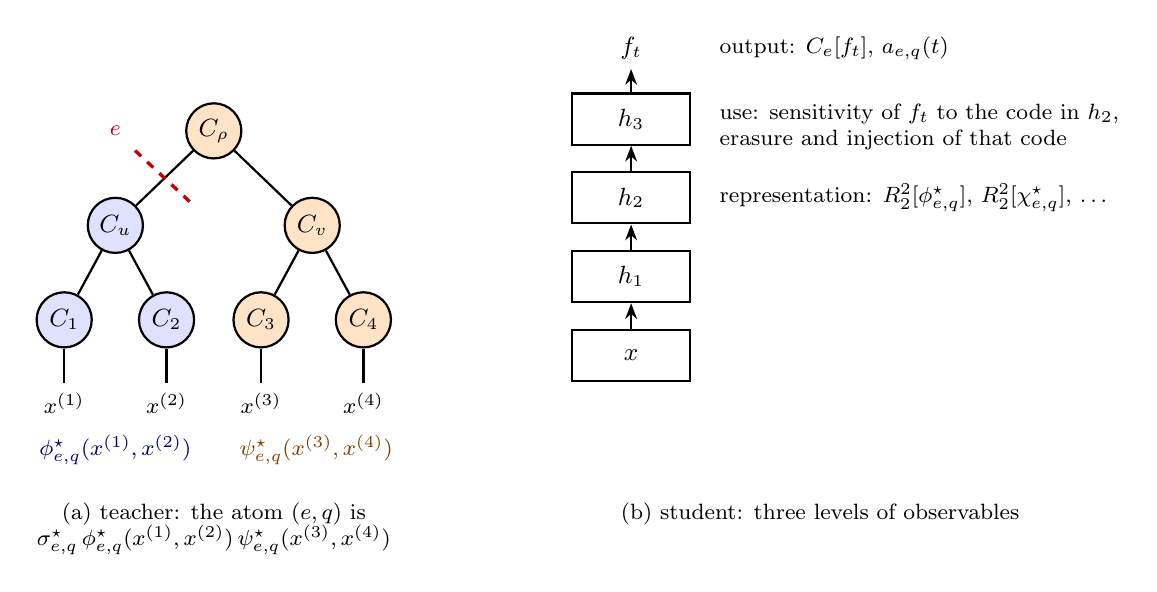
\begin{tikzpicture}[
  core/.style={circle, draw, thick, minimum size=7mm, inner sep=0pt, font=\small},
  insub/.style={core, fill=blue!12},
  outsub/.style={core, fill=orange!22},
  layer/.style={rectangle, draw, thick, fill=white, minimum width=15mm, minimum height=6.5mm, font=\small},
  lab/.style={font=\footnotesize},
  arr/.style={-{Stealth[length=2mm]}, thick}]
  % (a) teacher
  \node[outsub] (r) at (0,2.4) {$C_\rho$};
  \node[insub] (u) at (-1.25,1.2) {$C_u$};
  \node[outsub] (v) at (1.25,1.2) {$C_v$};
  \node[insub] (c1) at (-1.9,0) {$C_1$};
  \node[insub] (c2) at (-0.6,0) {$C_2$};
  \node[outsub] (c3) at (0.6,0) {$C_3$};
  \node[outsub] (c4) at (1.9,0) {$C_4$};
  \foreach \i/\xx in {1/-1.9, 2/-0.6, 3/0.6, 4/1.9} {
    \draw[thick] (c\i) -- (\xx,-0.8) node[below, lab] {$x^{(\i)}$};
  }
  \draw[thick] (r) -- (u) (r) -- (v) (u) -- (c1) (u) -- (c2) (v) -- (c3) (v) -- (c4);
  \draw[red!75!black, dashed, very thick] (-1.0,2.15) -- (-0.25,1.45);
  \node[lab, red!75!black] at (-1.25,2.4) {$e$};
  \node[lab, blue!50!black] at (-1.25,-1.65) {$\phi^\star_{e,q}(x^{(1)},x^{(2)})$};
  \node[lab, orange!50!black] at (1.3,-1.65) {$\psi^\star_{e,q}(x^{(3)},x^{(4)})$};
  \node[lab, align=center, anchor=north] at (0,-2.2) {(a) teacher: the atom $(e,q)$ is\\$\sigma^\star_{e,q}\,\phi^\star_{e,q}(x^{(1)},x^{(2)})\,\psi^\star_{e,q}(x^{(3)},x^{(4)})$};
  % (b) student
  \begin{scope}[xshift=5.3cm]
    \node[layer] (h0) at (0,-0.45) {$x$};
    \node[layer] (h1) at (0,0.55) {$h_1$};
    \node[layer] (h2) at (0,1.55) {$h_2$};
    \node[layer] (h3) at (0,2.55) {$h_3$};
    \node[font=\small] (f) at (0,3.45) {$f_t$};
    \draw[arr] (h0) -- (h1);
    \draw[arr] (h1) -- (h2);
    \draw[arr] (h2) -- (h3);
    \draw[arr] (h3) -- (f);
    \node[lab, anchor=west] at (1.0,3.45) {output: $C_e[f_t]$, $a_{e,q}(t)$};
    \node[lab, anchor=west, align=left] at (1.0,2.45) {use: sensitivity of $f_t$ to the code in $h_2$,\\erasure and injection of that code};
    \node[lab, anchor=west] at (1.0,1.55) {representation: $R^2_2[\phi^\star_{e,q}]$, $R^2_2[\chi^\star_{e,q}]$, \dots};
    \node[lab, align=center, anchor=north] at (2.4,-2.2) {(b) student: three levels of observables};
  \end{scope}
\end{tikzpicture}
\caption{Comparing a student with a TTN teacher. (a) Cutting the bond $e$ splits the teacher into the subtree below $e$ (blue), which computes the left factors $\phi^\star_{e,q}$ of the inputs $x^{(1)},x^{(2)}$, and its environment (orange), which computes the right factors $\psi^\star_{e,q}$ of $x^{(3)},x^{(4)}$. An atom is the product of two such factors, weighted by a singular value of the data-weighted HSVD (Sections~\ref{sec:dw-hsvd} and~\ref{sec:atoms}). (b) For a student, one asks whether its output contains the atom (Section~\ref{sec:output-obs}), whether the factors and the atom can be read off a hidden layer, here $h_2$ (Section~\ref{sec:representation}), and whether the layers above use and rely on that code (Section~\ref{sec:use}).}
\label{fig:compare}
\end{figure}

%----------------------------------------------------------------------
\subsection{The teacher--student setting}\label{sec:compare-setting}
%----------------------------------------------------------------------

\paragraph{Teacher.}
Fix a binary tree whose $N$ leaves carry one open leg each, indexed by $a\in[N]$; a balanced tree, with $N$ a power of two, is the simplest choice. We root the tree at an internal vertex $\rho$ and, as in Proposition~\ref{prop:nested}, let $A_e$ be the set of legs below the bond $e$, so that $A_e$ and $A_e^c$ are the two sides of the cut of Lemma~\ref{lem:cut}. A TTN on this tree (Definition~\ref{def:ttn}) represents a tensor $T^\star$. Leg $a$ receives the block $x^{(a)}\in\mathcal X_a$ of the input through a fixed embedding $\xi_a:\mathcal X_a\to\R^{d_a}$, for example $\xi_a(z)=z$ or $\xi_a(z)=(1,z)$, and, as in~\eqref{eq:ttn-model}, the teacher is
\begin{equation}\label{eq:teacher}
f^\star(x)=\Big\langle T^\star,\ \bigotimes_{a=1}^N\xi_a\big(x^{(a)}\big)\Big\rangle .
\end{equation}
The labels are $y=f^\star(x)$, possibly plus independent zero-mean noise. This is a \emph{physical} TTN in the sense of Section~\ref{sec:tn}: distinct legs receive distinct blocks of the input. For example, the balanced bilinear teacher of \citet[Section~6.2]{hfl_surrogate}, which applies linear maps at the leaves, planted bilinear maps at the internal vertices and a linear readout at the root, is of this form with $\xi_a(z)=z$.

\paragraph{Data.}
We assume throughout that the blocks are independent:
\begin{equation}\label{eq:independent-blocks}
\nu_x=\mu_1\otimes\cdots\otimes\mu_N,\qquad\E\norm{\xi_a(X^{(a)})}^2<\infty\quad(a\in[N]).
\end{equation}
The blocks need not be Gaussian, centred, whitened or identically distributed. For $A\subseteq[N]$, we write $x_A=(x^{(a)})_{a\in A}$, $\mu_A=\bigotimes_{a\in A}\mu_a$ and $\Xi_A(x_A)=\bigotimes_{a\in A}\xi_a(x^{(a)})$, and $X\sim\nu_x$ denotes a random input. Norms and inner products of functions are those of $L^2(\nu_x)$, or of $L^2(\mu_A)$ for functions of $x_A$. Assumption~\eqref{eq:independent-blocks} holds by construction in synthetic experiments. It is what makes the features of the teacher canonical functions of disjoint groups of input variables; Remark~\ref{rem:scope} discusses what is lost without it.

\paragraph{Students.}
A DNN $f_\theta$ of the form~\eqref{eq:network}, with a standard activation, and a TTN $g_\vartheta$ of the form~\eqref{eq:ttn-model}, normally on the teacher's tree, are trained on the same data, with the same loss and optimizer, and compared in the same time variable $t$, without time warping, as in Hypothesis~\ref{hyp:global}. We write $f_t$ for the predictor of a student at time $t$, whichever its architecture: $f_t=f_{\theta(t)}$ or $f_t=g_{\vartheta(t)}$. Three precautions apply \citep[Sections~6.6 and~6.7]{hfl_surrogate}. Every student should be able to fit the teacher under a generous training budget, since an underfitting student says nothing about dynamics. There is no single notion of equal capacity for a DNN and a TTN, so widths, ranks and initialization scales should be bracketed rather than matched by one number. Finally, a TTN on a wrong tree is a useful structural control.

%----------------------------------------------------------------------
\subsection{The data-weighted HSVD of the teacher}\label{sec:dw-hsvd}
%----------------------------------------------------------------------

Fix a bond $e$ of the teacher. It splits the legs into the legs $A_e$ below $e$ and the others, $A_e^c$, and contracting~\eqref{eq:teacher} gives, up to the ordering of the legs,
\begin{equation}\label{eq:teacher-cut}
f^\star(x)=\Xi_{A_e}(x_{A_e})^\top M^\star_e\,\Xi_{A_e^c}(x_{A_e^c}),\qquad M^\star_e:=T^{\star\langle A_e\rangle}.
\end{equation}
The HSVD of Definition~\ref{def:hsvd} decomposes $M^\star_e$ in the Euclidean geometry of coefficients. This is the right geometry for comparing tensors, but not for comparing functions: learning is driven by the population loss, hence by the geometry of $L^2(\nu_x)$. The two geometries agree when the leaf embeddings are orthonormal under the data, $\E[\xi_a\xi_a^\top]=I$, for instance for whitened inputs and $\xi_a(z)=z$. Otherwise they differ, and the Euclidean singular values can be misleading about which features matter (Example~\ref{ex:dw}). We therefore re-express the teacher in leaf bases that are orthonormal under the data, and take the HSVD there. No preprocessing is applied to the inputs seen by the students: the change of basis only concerns the coordinates in which we describe the teacher.

\begin{definition}[Data-weighted HSVD]\label{def:dw-hsvd}
For $a\in[N]$, let $\Sigma_a:=\E\big[\xi_a(X^{(a)})\,\xi_a(X^{(a)})^\top\big]$ be the Gram matrix of the embedding of leg $a$, and let $\Sigma_A:=\bigotimes_{a\in A}\Sigma_a$ for $A\subseteq[N]$. Write $(\cdot)^{1/2}$ for the positive semidefinite square root and $(\cdot)^+$ for the Moore--Penrose pseudoinverse. The \emph{whitened embeddings} are $\tilde\xi_a:=(\Sigma_a^{1/2})^+\xi_a$, with $\tilde\Xi_A:=\bigotimes_{a\in A}\tilde\xi_a$, and the \emph{data-weighted tensor} $\tilde T^\star$ is obtained from $T^\star$ by multiplying each leg $a$ by $\Sigma_a^{1/2}$. For each bond $e$, let
\[
\tilde M^\star_e:=\tilde T^{\star\langle A_e\rangle}=U^\star_eS^\star_eV^{\star\top}_e,\qquad
S^\star_e=\diag\big(\sigma^\star_{e,1},\dots,\sigma^\star_{e,r^\star_e}\big),\quad\sigma^\star_{e,1}\ge\dots\ge\sigma^\star_{e,r^\star_e}>0,
\]
be a compact SVD, with columns $u^\star_{e,q}$ of $U^\star_e$ and $v^\star_{e,q}$ of $V^\star_e$. The \emph{singular functions} of the teacher at $e$ are
\begin{equation}\label{eq:singular-functions}
\phi^\star_{e,q}(x_{A_e}):=u^{\star\top}_{e,q}\,\tilde\Xi_{A_e}(x_{A_e}),\qquad
\psi^\star_{e,q}(x_{A_e^c}):=v^{\star\top}_{e,q}\,\tilde\Xi_{A_e^c}(x_{A_e^c}),\qquad q\le r^\star_e .
\end{equation}
The family $(\sigma^\star_{e,q},\phi^\star_{e,q},\psi^\star_{e,q})_{e\in\Eint,\,q\le r^\star_e}$ is the \emph{data-weighted HSVD} of the teacher.
\end{definition}

For $\xi_a(z)=(1,z)$, $\Sigma_a$ is the matrix of the first and second moments of $x^{(a)}$, whatever its distribution. In general, $\Sigma_a$ is computed analytically or estimated once, from a large sample independent of all other data.

\begin{proposition}[Properties of the data-weighted HSVD]\label{prop:dw-hsvd}
Under~\eqref{eq:independent-blocks}:
\begin{enumerate}[label=(\roman*),nosep]
\item $\E\big[\Xi_A(X_A)\,\Xi_A(X_A)^\top\big]=\Sigma_A$ for every $A\subseteq[N]$, and $\tilde M^\star_e=\Sigma_{A_e}^{1/2}M^\star_e\,\Sigma_{A_e^c}^{1/2}$ for every bond $e$.
\item $\tilde T^\star$ is represented by the teacher TTN in which the open leg of each leaf core is multiplied by $\Sigma_a^{1/2}$, with the same tree and bond dimensions. Hence the data-weighted HSVD is the HSVD of a TTN: Propositions~\ref{prop:nested} and~\ref{prop:truncation} and Remark~\ref{rem:stability} apply to it, and it is gauge invariant.
\item $f^\star(x)=\big\langle\tilde T^\star,\bigotimes_a\tilde\xi_a(x^{(a)})\big\rangle$ for $\nu_x$-almost every $x$.
\item For every bond $e$, $(\phi^\star_{e,q})_q$ is orthonormal in $L^2(\mu_{A_e})$, $(\psi^\star_{e,q})_q$ is orthonormal in $L^2(\mu_{A_e^c})$, and
\begin{equation}\label{eq:dw-expansion}
f^\star(x)=\sum_{q=1}^{r^\star_e}\sigma^\star_{e,q}\,\phi^\star_{e,q}(x_{A_e})\,\psi^\star_{e,q}(x_{A_e^c})\qquad\text{for $\nu_x$-almost every $x$.}
\end{equation}
\item The expansion~\eqref{eq:dw-expansion} is the Schmidt decomposition of $f^\star$ across the physical cut $(A_e\mid A_e^c)$ of Remark~\ref{rem:which-tensor}: $\sigma^\star_{e,q}=s_q(f^\star)$, and $r^\star_e$ is the rank of $f^\star$ across the cut. The singular values, and the spans of the singular functions that belong to equal singular values, depend only on $f^\star$, $\nu_x$ and the bipartition. In particular, they depend neither on the gauge nor on the choice of the embeddings $\xi_a$, as long as $f^\star$ is unchanged.
\end{enumerate}
\end{proposition}

\begin{proof}
(i) By independence, $\E\big[\bigotimes_{a\in A}\xi_a\xi_a^\top\big]=\bigotimes_{a\in A}\E[\xi_a\xi_a^\top]$. Matricizing $\tilde T^\star$ across $(A_e\mid A_e^c)$ gives $\big(\bigotimes_{a\in A_e}\Sigma_a^{1/2}\big)M^\star_e\big(\bigotimes_{a\in A_e^c}\Sigma_a^{1/2}\big)$, and the Kronecker product of the square roots of positive semidefinite matrices is the square root of their Kronecker product. (ii) Multiplying an open leg of a core by a matrix multiplies the corresponding mode of the contraction~\eqref{eq:contraction} by that matrix. Since $\tilde T^\star$ is determined by $T^\star$, it is gauge invariant (Proposition~\ref{prop:gauge}). (iii) Let $\Pi_a:=\Sigma_a^{1/2}(\Sigma_a^{1/2})^+$ be the orthogonal projector onto the range of $\Sigma_a$. If $\Sigma_aw=0$, then $\E[(w^\top\xi_a)^2]=w^\top\Sigma_aw=0$, so $\xi_a(X^{(a)})$ lies in the range of $\Sigma_a$ almost surely, i.e.\ $\Pi_a\xi_a=\xi_a$. Hence $\langle\tilde T^\star,\bigotimes_a\tilde\xi_a\rangle=\langle T^\star,\bigotimes_a\Pi_a\xi_a\rangle=f^\star$ almost surely. (iv) By (i), $\E[\tilde\Xi_A\tilde\Xi_A^\top]=\bigotimes_{a\in A}(\Sigma_a^{1/2})^+\Sigma_a(\Sigma_a^{1/2})^+=\bigotimes_{a\in A}\Pi_a=:\Pi_A$, the orthogonal projector onto the range of $\Sigma_A^{1/2}$. The columns of $U^\star_e$ lie in $\col(\tilde M^\star_e)$, which is contained in that range, so $\E[\phi^\star_{e,q}\phi^\star_{e,q'}]=u^{\star\top}_{e,q}\Pi_{A_e}u^\star_{e,q'}=\delta_{qq'}$; the same argument applies to the $\psi^\star_{e,q}$. By (iii), $f^\star=\tilde\Xi_{A_e}^\top\tilde M^\star_e\tilde\Xi_{A_e^c}$ almost surely, and inserting the SVD gives~\eqref{eq:dw-expansion}. (v) Under~\eqref{eq:independent-blocks}, $L^2(\nu_x)=L^2(\mu_{A_e})\otimes L^2(\mu_{A_e^c})$, and $f^\star$ is the kernel of a Hilbert--Schmidt operator $K_{f^\star}:L^2(\mu_{A_e^c})\to L^2(\mu_{A_e})$, $(K_{f^\star}\psi)(x_{A_e})=\E[f^\star(x_{A_e},X_{A_e^c})\,\psi(X_{A_e^c})]$. By (iv), $K_{f^\star}K_{f^\star}^*=\sum_q\sigma^{\star2}_{e,q}\,\phi^\star_{e,q}\langle\phi^\star_{e,q},\cdot\rangle$, so the $\sigma^{\star2}_{e,q}$ are the nonzero eigenvalues of $K_{f^\star}K_{f^\star}^*$, with eigenspaces spanned by the $\phi^\star_{e,q}$ of equal $\sigma^\star_{e,q}$. These are determined by $f^\star$ and $\nu_x$. The same argument with $K_{f^\star}^*K_{f^\star}$ applies to the $\psi^\star_{e,q}$.
\end{proof}

When all $\Sigma_a$ are invertible, $r^\star_e=\rank M^\star_e$. When some $\Sigma_a$ is singular, which happens when the embedding is redundant on the support of the data, $r^\star_e$ can be smaller than $\rank M^\star_e$: directions of coefficients that vanish on the data do not count.

\begin{example}[Why the data weighting matters]\label{ex:dw}
Take $N=2$ blocks $x^{(1)},x^{(2)}\in\R^2$, $\xi_a(z)=z$, and the teacher $f^\star(x)=\langle x^{(1)},x^{(2)}\rangle=x^{(1)}_1x^{(2)}_1+x^{(1)}_2x^{(2)}_2$, a TTN with two leaves and one bond. Its coefficient matrix is $M^\star=I_2$, so the Euclidean HSVD has a degenerate pair $\sigma_1=\sigma_2=1$ and suggests two equally important atoms, $x^{(1)}_1x^{(2)}_1$ and $x^{(1)}_2x^{(2)}_2$. Now let $x^{(2)}\sim\mathcal N(0,I_2)$ and $x^{(1)}\sim\mathcal N(0,\Sigma_1)$ with $\Sigma_1=\left(\begin{smallmatrix}1&\rho\\\rho&1\end{smallmatrix}\right)$ and $0<\rho<1$. Then $\tilde M^\star=\Sigma_1^{1/2}$ has the singular values $\sqrt{1+\rho}$ and $\sqrt{1-\rho}$, and
\[
f^\star=\sqrt{1+\rho}\;\phi^\star_+\psi^\star_++\sqrt{1-\rho}\;\phi^\star_-\psi^\star_-,\qquad
\phi^\star_\pm=\frac{x^{(1)}_1\pm x^{(1)}_2}{\sqrt{2(1\pm\rho)}},\qquad
\psi^\star_\pm=\frac{x^{(2)}_1\pm x^{(2)}_2}{\sqrt2}.
\]
Under the data, there is one strong atom, which carries the fraction $(1+\rho)/2$ of $\norm{f^\star}^2$, and one weak atom. For $\rho$ close to $1$, the best predictor of rank one across the cut already has the small population loss $(1-\rho)/2$ (Proposition~\ref{prop:atoms}(iii) below). Which atoms the loss favours, and plausibly which atoms a loss-driven learner acquires first, is decided by the data-weighted singular values, not by the Euclidean ones.
\end{example}

\begin{remark}[Why only second moments appear]\label{rem:second-moments}
The data enter the data-weighted HSVD only through the Gram matrices $\Sigma_a$. This is not a Gaussian assumption. It holds because a physical TTN is linear in each leaf embedding separately: for two functions $g=\langle T,\bigotimes_a\xi_a\rangle$ and $h=\langle T',\bigotimes_a\xi_a\rangle$, independence gives
\[
\E[g(X)h(X)]=\vect(T)^\top\Big(\bigotimes_{a=1}^N\Sigma_a\Big)\vect(T').
\]
Moreover, $\Sigma_a$ is a second moment of the \emph{embedding}, not of the raw input: for a scalar block and $\xi_a(z)=(1,z,z^2,z^3)$, it contains the moments of $z$ up to order six. Higher joint moments enter as soon as this multilinear structure in independent variables is lost: when blocks are dependent, or when the same input feeds several legs, as in the computational TTN of a DPN (Remark~\ref{rem:copies}), whose $L^2$ geometry involves the moments of $x$ up to twice the number of copies of the input \citep[Section~8.1]{hfl_local}.
\end{remark}

\begin{remark}[Features of the teacher are built from features of the teacher]\label{rem:dw-nested}
By Proposition~\ref{prop:dw-hsvd}(ii), Proposition~\ref{prop:nested} applies to $\tilde T^\star$. Let $u$ be an internal vertex with parent bond $e$ and child bonds $e_1,e_2$, and let $B_u:=(U^\star_{e_1}\otimes U^\star_{e_2})^\top U^\star_e$. Since $U^\star_e=(U^\star_{e_1}\otimes U^\star_{e_2})B_u$ and $\tilde\Xi_{A_e}=\tilde\Xi_{A_{e_1}}\otimes\tilde\Xi_{A_{e_2}}$ up to the ordering of the legs,
\begin{equation}\label{eq:feature-composition}
\phi^\star_{e,q}(x_{A_e})=\sum_{i\le r^\star_{e_1}}\ \sum_{j\le r^\star_{e_2}}(B_u)_{(i,j),q}\;\phi^\star_{e_1,i}(x_{A_{e_1}})\,\phi^\star_{e_2,j}(x_{A_{e_2}}).
\end{equation}
Each left singular function is thus a \emph{bilinear} function of the left singular functions at the two bonds below it. At a \emph{leaf bond}, i.e.\ a bond $e$ that joins a leaf $a$ to its parent, $A_e=\{a\}$ and $\phi^\star_{e,q}=u^{\star\top}_{e,q}\tilde\xi_a$ is linear in the embedding. This is the precise sense in which the features of the teacher are hierarchical, and it motivates looking for them in successive layers of a DNN (Hypothesis~\ref{hyp:layer-bond}). The two child bonds of the root define the same bipartition, with left and right exchanged, and therefore have the same singular values and atoms.
\end{remark}

\begin{remark}[Computing the data-weighted HSVD]\label{rem:dw-compute}
The matrices $\tilde M^\star_e$ are exponentially large and are never formed. One multiplies the leaf cores by $\Sigma_a^{1/2}$ (Proposition~\ref{prop:dw-hsvd}(ii)), orthonormalizes the network towards $e$ by QR decompositions, and takes the SVD of the resulting small centre matrix \citep{grasedyck2010hierarchical}, \citep[Section~9.2]{hfl_diagonal}. The values of the singular functions at a sample are obtained by contracting the two orthonormalized halves of the network with the whitened embeddings $\tilde\xi_a(x^{(a)})$ and rotating the results by the singular vectors of the centre matrix. The cost is polynomial in the bond and leg dimensions and linear in $N$.
\end{remark}

%----------------------------------------------------------------------
\subsection{Atoms: identity and strength}\label{sec:atoms}
%----------------------------------------------------------------------

\begin{definition}[Atoms]\label{def:atom}
For a bond $e$ and $i,j\le r^\star_e$, let $\chi^\star_{e,ij}(x):=\phi^\star_{e,i}(x_{A_e})\,\psi^\star_{e,j}(x_{A_e^c})$, and $\chi^\star_{e,q}:=\chi^\star_{e,qq}$. The \emph{atom} $(e,q)$ of the teacher is the function $\sigma^\star_{e,q}\chi^\star_{e,q}$. We call $\chi^\star_{e,q}$ the \emph{normalized atom}, $\phi^\star_{e,q}$ its \emph{left factor} and $\psi^\star_{e,q}$ its \emph{right factor}.
\end{definition}

An atom is one mode of the data-weighted SVD at one bond: one ``atom of computation'' of the teacher. Its left factor is a function computed by the subtree below $e$, its right factor is a function computed by the rest of the tree, and the atom is their product, weighted by the strength $\sigma^\star_{e,q}$ with which the two sides are coupled.

\begin{proposition}[Atoms]\label{prop:atoms}
Under~\eqref{eq:independent-blocks}, for every bond $e$:
\begin{enumerate}[label=(\roman*),nosep]
\item the functions $\chi^\star_{e,ij}$, $i,j\le r^\star_e$, are orthonormal in $L^2(\nu_x)$; in particular $\norm{\chi^\star_{e,q}}=1$ and $\norm{\sigma^\star_{e,q}\chi^\star_{e,q}}=\sigma^\star_{e,q}$;
\item $f^\star=\sum_{q\le r^\star_e}\sigma^\star_{e,q}\chi^\star_{e,q}$ and $\norm{f^\star}^2=\sum_q\sigma^{\star2}_{e,q}$;
\item for $r<r^\star_e$, the truncation $f^\star_{e,r}:=\sum_{q\le r}\sigma^\star_{e,q}\chi^\star_{e,q}$ minimizes $\norm{f^\star-g}$ over the functions $g\in L^2(\nu_x)$ of rank at most $r$ across $(A_e\mid A_e^c)$, i.e.\ of the form $g=\sum_{k\le r}a_k(x_{A_e})\,b_k(x_{A_e^c})$, and $\norm{f^\star-f^\star_{e,r}}^2=\sum_{q>r}\sigma^{\star2}_{e,q}$.
\end{enumerate}
\end{proposition}

\begin{proof}
(i) By the independence of $X_{A_e}$ and $X_{A_e^c}$ and Proposition~\ref{prop:dw-hsvd}(iv),
\[
\E\big[\chi^\star_{e,ij}\chi^\star_{e,kl}\big]=\E\big[\phi^\star_{e,i}\phi^\star_{e,k}\big]\,\E\big[\psi^\star_{e,j}\psi^\star_{e,l}\big]=\delta_{ik}\delta_{jl}.
\]
(ii) follows from~\eqref{eq:dw-expansion} and (i). (iii) is the Eckart--Young theorem \citep{eckart1936approximation}, which holds verbatim for Hilbert--Schmidt operators, applied to the operator $K_{f^\star}$ of the proof of Proposition~\ref{prop:dw-hsvd}(v): its approximations of rank at most $r$ are exactly the kernels of rank at most $r$ across the cut.
\end{proof}

\paragraph{Identity and strength.}
The normalized factors $\phi^\star_{e,q}$ and $\psi^\star_{e,q}$ specify \emph{which} computation the atom performs on each side of the interface; the singular value specifies its \emph{strength}. By Proposition~\ref{prop:atoms}, $\sigma^{\star2}_{e,q}$ is the part of the teacher's second moment $\E[f^\star(X)^2]=\norm{f^\star}^2$ carried by the atom, and replacing the truncation $f^\star_{e,q-1}$ by $f^\star_{e,q}$, i.e.\ adding the atom to the stronger atoms at $e$, lowers the population loss $\mathcal L(f)=\frac12\E[(f(x)-y)^2]$ by $\sigma^{\star2}_{e,q}/2$. A student can have acquired the identity of an atom, for instance by computing its factors internally, without having amplified it in its output; conversely, its output can contain a weak version of the right atom. Direction acquisition and amplification must therefore be tracked separately \citep[Sections~3.2 and~9.4]{hfl_diagonal}.

\begin{remark}[Degenerate atoms]\label{rem:degenerate}
If $\sigma^\star_{e,q}$ is a simple singular value, then $(\phi^\star_{e,q},\psi^\star_{e,q})$ is unique up to a simultaneous change of sign, which leaves $\chi^\star_{e,q}$ unchanged: the atom is canonical. If instead a block $B$ of $k\ge2$ singular values equals a common value $\sigma^\star_B$, then $(U^\star_{e,B}R,\,V^\star_{e,B}R)$ is another valid choice of the corresponding singular vectors for any $R\in\mathrm O(k)$ (Remark~\ref{rem:hsvd-canonical}). The canonical objects are then the left and right subspaces $\operatorname{span}\{\phi^\star_{e,q}:q\in B\}$ and $\operatorname{span}\{\psi^\star_{e,q}:q\in B\}$, and the \emph{block atom} $\sigma^\star_B\sum_{q\in B}\chi^\star_{e,q}$, which is invariant because $\sum_q(UR)_{:,q}\otimes(VR)_{:,q}=\sum_qu_q\otimes v_q$ when $RR^\top=I$. Individual atoms inside a degenerate block have no separate meaning, and Example~\ref{ex:modular} shows that such blocks occur in natural tasks. When singular values are distinct but their gaps are comparable to the estimation error, the cluster should also be treated as a block, since singular functions are stable only relative to the gaps (Remark~\ref{rem:stability}); the strengths within the cluster are then described by the corresponding diagonal block $S^\star_{e,BB}$ of $S^\star_e$ rather than by a common value. The observables below have block versions, which reduce to single atoms for simple singular values.
\end{remark}

\begin{remark}[Atoms are attached to bonds]\label{rem:edge-specific}
For each bond $e$, Proposition~\ref{prop:atoms}(ii) decomposes the same function $f^\star$ into orthonormal features with strengths, exactly as in~\eqref{eq:acquisition}, with $\chi_m=\chi^\star_{e,q}$ and $\lambda_m=\sigma^{\star2}_{e,q}$. Different bonds give different decompositions. The teacher therefore supplies not one flat dictionary of features but one decomposition per bond, and these decompositions are linked by the nestedness~\eqref{eq:feature-composition}. Accordingly, observables are indexed by a bond and a mode, or a block.
\end{remark}

%----------------------------------------------------------------------
\subsection{Output observables: has the predictor acquired an atom?}\label{sec:output-obs}
%----------------------------------------------------------------------

The most direct question is whether the predictor $f_t$ of a student contains the atom $\sigma^\star_{e,q}\chi^\star_{e,q}$. The distance $\norm{f_t-\sigma^\star_{e,q}\chi^\star_{e,q}}$ is not the right observable: a student that has learned this atom \emph{and} the other ones is far from it, since $\norm{f^\star-\sigma^\star_{e,q}\chi^\star_{e,q}}^2=\sum_{q'\neq q}\sigma^{\star2}_{e,q'}$. The right operation is a projection, which measures the component of $f_t$ along the atom. Since a student can also couple the teacher's factors in ways that the teacher does not, pairing $\phi^\star_{e,i}$ with $\psi^\star_{e,j}$ for $i\neq j$, we measure all pairings at once.

\begin{definition}[Coupling matrix and output acquisition coefficients]\label{def:coupling}
Let $\Phi^\star_e:=(\phi^\star_{e,1},\dots,\phi^\star_{e,r^\star_e})^\top$ and $\Psi^\star_e:=(\psi^\star_{e,1},\dots,\psi^\star_{e,r^\star_e})^\top$. The \emph{coupling matrix} of a function $f\in L^2(\nu_x)$ at the bond $e$ is
\begin{equation}\label{eq:coupling}
C_e[f]:=\E\Big[f(X)\,\Phi^\star_e(X_{A_e})\,\Psi^\star_e(X_{A_e^c})^\top\Big]\in\R^{r^\star_e\times r^\star_e},\qquad\text{i.e.}\quad C_e[f]_{ij}=\langle f,\chi^\star_{e,ij}\rangle .
\end{equation}
Along a trajectory $f_t$, the \emph{output acquisition coefficients} of the atom $(e,q)$ and of a block $B$ (a set of equal, or nearly equal, singular values) are
\[
a_{e,q}(t):=\frac{C_e[f_t]_{qq}}{\sigma^\star_{e,q}}=\frac{\langle f_t,\chi^\star_{e,q}\rangle}{\sigma^\star_{e,q}},\qquad
a_{e,B}(t):=\frac{\operatorname{tr}C_e[f_t]_{BB}}{\operatorname{tr}S^\star_{e,BB}},
\]
where $C_{BB'}$ denotes the submatrix of a matrix $C$ with rows in $B$ and columns in $B'$. For a block of equal singular values, $\operatorname{tr}S^\star_{e,BB}=|B|\,\sigma^\star_B$.
\end{definition}

By Remark~\ref{rem:edge-specific}, $a_{e,q}$ is the coefficient~\eqref{eq:acquisition} of the decomposition of $f^\star$ at $e$: $a_{e,q}(t)=0$ means that the atom is absent from the predictor, and $a_{e,q}(t)=1$ that it is present with the teacher's strength. The coupling matrix contains more information than these coefficients.

\begin{proposition}[Exact error decomposition at a bond]\label{prop:error-decomposition}
Assume~\eqref{eq:independent-blocks}, and let $\Pi_e$ be the orthogonal projector of $L^2(\nu_x)$ onto $\operatorname{span}\{\chi^\star_{e,ij}:i,j\le r^\star_e\}$, the tensor product of the span of the left singular functions at $e$ with the span of the right ones. For every $f\in L^2(\nu_x)$:
\begin{enumerate}[label=(\roman*),nosep]
\item $\Pi_ef=\Phi^{\star\top}_e\,C_e[f]\,\Psi^\star_e$ and $\norm{\Pi_ef}^2=\norm{C_e[f]}_F^2$;
\item $C_e[f^\star]=S^\star_e$;
\item writing $C=C_e[f]$, $S^\star=S^\star_e$, and letting $B,B'$ range over the blocks of a partition of the modes $\{1,\dots,r^\star_e\}$,
\begin{equation}\label{eq:error-decomposition}
\norm{f-f^\star}^2=\underbrace{\sum_B\norm{C_{BB}-S^\star_{BB}}_F^2}_{\text{within blocks}}+\underbrace{\sum_{B\neq B'}\norm{C_{BB'}}_F^2}_{\text{across blocks}}+\underbrace{\norm{f}^2-\norm{C}_F^2}_{\text{outside}};
\end{equation}
when all blocks are single modes, the first two terms are $\sum_q\sigma^{\star2}_{e,q}(a_{e,q}-1)^2$, with $a_{e,q}=C_{qq}/\sigma^\star_{e,q}$, and $\sum_{i\neq j}C_{ij}^2$;
\item if the blocks are the sets of equal singular values, the three terms of~\eqref{eq:error-decomposition}, the block coefficients $\operatorname{tr}C_{BB}/\operatorname{tr}S^\star_{BB}$ and the singular values of $C$ do not depend on the choices of singular functions allowed by Remark~\ref{rem:degenerate}.
\end{enumerate}
\end{proposition}

\begin{proof}
(i) By Proposition~\ref{prop:atoms}(i), the $\chi^\star_{e,ij}$ form an orthonormal basis of the range of $\Pi_e$, and the $C_e[f]_{ij}$ are the coordinates of $\Pi_ef$ in this basis. (ii) follows from Proposition~\ref{prop:atoms}(i) and~(ii). (iii) Since $f^\star$ lies in the range of $\Pi_e$, $f-f^\star=(\Pi_ef-f^\star)+(f-\Pi_ef)$ is an orthogonal decomposition. By (i), $\norm{f-\Pi_ef}^2=\norm f^2-\norm{C}_F^2$, and by (i), (ii) and orthonormality, $\norm{\Pi_ef-f^\star}^2=\norm{C-S^\star_e}_F^2$. Since $S^\star_e$ is diagonal, its off-diagonal blocks vanish, and splitting $\norm{C-S^\star_e}_F^2$ into blocks gives the first two terms. (iv) An allowed change of singular functions replaces $\Phi^\star_e$ and $\Psi^\star_e$ by $R^\top\Phi^\star_e$ and $R^\top\Psi^\star_e$, where $R$ is block diagonal and orthogonal: a sign for each simple singular value and some $R_B\in\mathrm O(|B|)$ for each block. Then $C\mapsto R^\top CR$, i.e.\ $C_{BB'}\mapsto R_B^\top C_{BB'}R_{B'}$, and $S^\star_{BB}=\sigma^\star_BI$ is unchanged; this preserves the Frobenius norm of every block of $C$ and of $C-S^\star$, the traces of the diagonal blocks and the singular values of $C$, while $\Pi_e$ depends only on the spans.
\end{proof}

\paragraph{Interpretation.}
For noiseless labels, $\norm{f-f^\star}^2=2\mathcal L(f)$; with independent zero-mean label noise, it is twice the excess loss. For every bond $e$, with the blocks of equal singular values,~\eqref{eq:error-decomposition} therefore splits the excess loss of a student into three parts, all of which can be read off $C_e[f_t]$ and $\norm{f_t}^2$:
\begin{enumerate}[label=(\alph*),nosep]
\item an error \emph{within blocks}: for a simple singular value, the student pairs the teacher's factors correctly but with the wrong strength, typically because the atom has not yet been amplified ($a_{e,q}<1$) or has overshot; for a degenerate block, this term also contains mispairings inside the block, since $C_{BB}=\sigma^\star_BR$ with an orthogonal $R\neq I$ has the right strengths and subspaces but pairs them differently from the teacher;
\item an error \emph{across blocks}: the student couples a left factor of the teacher with a right factor that belongs to a different singular value;
\item an \emph{outside} error: the energy of $f_t$ outside the teacher's factor spaces at $e$, i.e.\ the student uses functions of $x_{A_e}$ or of $x_{A_e^c}$ that the teacher does not use across this cut.
\end{enumerate}
Each bond gives a different split of the same number. Matching the coefficients $a_{e,q}$ while carrying a large outside error is not a success \citep[Section~7.1]{hfl_surrogate}, so the three terms should be reported together, for instance divided by $\norm{f^\star}^2=\norm{S^\star_e}_F^2$: the three fractions then add up to the relative error $\norm{f_t-f^\star}^2/\norm{f^\star}^2$, and how they split shows where the error lies at each bond. If only the leading $r<r^\star_e$ modes are used, (i)--(iii) hold with $C_e$ and $S^\star_e$ restricted to them, the last term becoming $\norm{(I-\Pi_{e,r})(f-f^\star)}^2$, where $\Pi_{e,r}$ is the projector onto the span of the $\chi^\star_{e,ij}$ with $i,j\le r$.

\begin{remark}[Removing an atom from the output is not informative]\label{rem:output-ablation}
One may try to assess whether an atom is useful to the student by removing the student's own component along it, $f^{(-q)}:=f-C_e[f]_{qq}\,\chi^\star_{e,q}$, and measuring the resulting change of the loss. For the square loss, with or without independent label noise, expanding the square and using $\langle f-f^\star,\chi^\star_{e,q}\rangle=C_e[f]_{qq}-\sigma^\star_{e,q}$ gives
\[
\mathcal L\big(f^{(-q)}\big)-\mathcal L(f)=\frac{\sigma^{\star2}_{e,q}}2\Big(1-\big(1-a_{e,q}\big)^2\Big),\qquad a_{e,q}=\frac{C_e[f]_{qq}}{\sigma^\star_{e,q}}.
\]
This is a function of $a_{e,q}$ alone: it is positive for $0<a_{e,q}<2$, maximal at $a_{e,q}=1$, and negative for $a_{e,q}<0$ or $a_{e,q}>2$. It carries no information beyond $a_{e,q}$, so causal questions have to be asked inside the network (Section~\ref{sec:use}).
\end{remark}

%----------------------------------------------------------------------
\subsection{The functional HSVD of a student}\label{sec:student-fsvd}
%----------------------------------------------------------------------

The coupling matrix describes a student in the coordinates of the teacher. A complementary, teacher-free description uses the student's own decomposition across the same cuts. Under~\eqref{eq:independent-blocks}, every $f\in L^2(\nu_x)$ has, for every bond $e$ of the teacher's tree, a Schmidt decomposition (Remark~\ref{rem:which-tensor})
\begin{equation}\label{eq:student-fsvd}
f(x)=\sum_{q\ge1}s_{e,q}(f)\,\phi^f_{e,q}(x_{A_e})\,\psi^f_{e,q}(x_{A_e^c}),
\end{equation}
with $s_{e,1}(f)\ge s_{e,2}(f)\ge\dots\ge0$ and orthonormal families $(\phi^f_{e,q})_q$ in $L^2(\mu_{A_e})$ and $(\psi^f_{e,q})_q$ in $L^2(\mu_{A_e^c})$. We call the family of these decompositions over the bonds of the teacher's tree the \emph{functional HSVD} of $f$ \citep[Section~7.4]{hfl_surrogate}, \citep[Section~9.2]{hfl_diagonal}. By Proposition~\ref{prop:dw-hsvd}(v), the functional HSVD of $f^\star$ is its data-weighted HSVD. For a student, it depends only on the predictor and on $\nu_x$, so it is defined in the same way for a DNN, for a TTN on any tree and for a polynomial surrogate, and its ranks are not bounded by any width. It describes what a student computes. The computational HSVD of Definition~\ref{def:features}, which describes how a polynomial network computes, is not used in this section.

\paragraph{Comparison with the teacher.}
The strengths $s_{e,q}(f_t)$ are compared with the $\sigma^\star_{e,q}$, and the directions through the alignment of the leading singular subspaces,
\[
\mathrm{Al}_{e,r}(t):=\frac1r\operatorname{tr}\big(P^{f_t}_{e,r}P^\star_{e,r}\big)\in[0,1],
\]
where $P^{f_t}_{e,r}$ and $P^\star_{e,r}$ are the orthogonal projectors of $L^2(\mu_{A_e})$ onto the spans of the $r$ leading left singular functions of $f_t$ and of $f^\star$, with $r$ chosen at a gap of both spectra \citep[Section~9.4]{hfl_diagonal}; right subspaces are compared in the same way. Alignment measures the acquisition of directions, and singular values measure amplification. Both are stable: the cut operator of $f-f^\star$ has Hilbert--Schmidt norm $\norm{f-f^\star}$, so $|s_{e,q}(f)-\sigma^\star_{e,q}|\le\norm{f-f^\star}$ by Weyl's inequality, and the deviation of the subspaces is controlled by the Davis--Kahan theorem relative to the gap \citep[Section~8.3]{hfl_local}. The coupling matrix sees the part of this decomposition that lies in the teacher's factor spaces: the singular values of $C_e[f]$ are those of $\Pi_ef$, and $s_{e,q}(\Pi_ef)\le s_{e,q}(f)$ for every $q$, because the cut operator of $\Pi_ef$ is that of $f$ multiplied on both sides by orthogonal projectors.

\paragraph{Estimation.}
Draw $x^{\mathrm L}_1,\dots,x^{\mathrm L}_{n_L}\sim\mu_{A_e}$ and $x^{\mathrm R}_1,\dots,x^{\mathrm R}_{n_R}\sim\mu_{A_e^c}$ independently, and form the crossed-grid matrix
\begin{equation}\label{eq:crossed-grid}
\hat K_e[f]:=\bigg[\frac{f(x^{\mathrm L}_k,x^{\mathrm R}_l)}{\sqrt{n_Ln_R}}\bigg]_{k\le n_L,\ l\le n_R}.
\end{equation}
If $\hat K_e[f]=\hat U\hat S\hat V^\top$, the singular values estimate the $s_{e,q}(f)$, and $\sqrt{n_L}\,\hat U_{:,q}$ and $\sqrt{n_R}\,\hat V_{:,q}$ estimate the values of $\phi^f_{e,q}$ at the $x^{\mathrm L}_k$ and of $\psi^f_{e,q}$ at the $x^{\mathrm R}_l$ \citep[Section~8.4]{hfl_local}. Indeed, substituting~\eqref{eq:student-fsvd} gives $\hat K_e[f]=\sum_qs_{e,q}(f)\,p_qw_q^\top$ with $p_q=\big(\phi^f_{e,q}(x^{\mathrm L}_k)/\sqrt{n_L}\big)_k$ and $w_q=\big(\psi^f_{e,q}(x^{\mathrm R}_l)/\sqrt{n_R}\big)_l$, and these vectors are orthonormal up to sampling error by the law of large numbers. Letting first $n_R$ and then $n_L$ tend to infinity reduces the consistency of the leading singular values to the convergence of the spectra of kernel matrices to those of integral operators \citep{koltchinskii2000random}. The same grid should be used for the teacher and all students. Since the $n_Ln_R$ entries share rows and columns, uncertainty should be estimated with independent grids or by resampling rows and columns, not by an i.i.d.\ bootstrap of the entries; a $64\times64$ grid with a stability check at $128\times128$ is a reasonable start \citep[Sections~9 and~10.2]{hfl_surrogate}.

\begin{remark}[Cost, and proxies for large inputs]\label{rem:fsvd-cost}
The size of $\hat K_e$ is chosen by the analyst and does not grow with the input dimension; the matrix costs $n_Ln_R$ evaluations of the student. The number of samples needed is set by the number of modes to resolve, by their gaps and by the tails of $f$, rather than by $\dim x$. When even this is too expensive, two proxies need only ordinary samples $X\sim\nu_x$. (a) The coupling matrix $C_e[f]$: an $r^\star_e\times r^\star_e$ matrix, whose Monte Carlo estimate from $M$ samples has error $O(M^{-1/2})$ when $f\,\phi^\star_{e,i}\psi^\star_{e,j}$ has finite variance. (b) More generally, a Galerkin version. Let $\Phi^D$ and $\Psi^D$ be finite families of functions of $x_{A_e}$ and of $x_{A_e^c}$, orthonormal in $L^2(\mu_{A_e})$ and $L^2(\mu_{A_e^c})$ and containing the teacher's singular functions. The SVD of $C^D_e[f]:=\E\big[f(X)\,\Phi^D(X_{A_e})\Psi^D(X_{A_e^c})^\top\big]$ is the functional SVD of the projection of $f$ onto $\operatorname{span}\Phi^D\otimes\operatorname{span}\Psi^D$, and the captured fraction $\norm{C^D_e[f]}_F^2/\norm f^2$ certifies how much of $f$ the dictionaries resolve. Natural dictionaries add products of whitened leaf embeddings, or orthonormal polynomials of the blocks, to the teacher's singular functions \citep[Section~8.2]{hfl_local}. As the dictionaries become complete, the projections converge to $f$, and their singular values and well-separated singular subspaces converge to those of~\eqref{eq:student-fsvd}.
\end{remark}

\begin{remark}[Scope: dependent inputs]\label{rem:scope}
Both $C_e$ and the functional HSVD rely on the independence~\eqref{eq:independent-blocks}: it makes the products $\chi^\star_{e,ij}$ orthonormal, makes $L^2(\nu_x)$ a tensor product across each cut, and makes the crossed grid sample from the data distribution. For real data, recombined inputs $(x^{\mathrm L}_k,x^{\mathrm R}_l)$ can be far from the data, and a factorization of $\nu_x$ is generally unknown, which is part of the reason for using DNNs in the first place. Conditional samplers, explicitly empirical operators or comparisons in representation space are then needed \citep[Section~6.5]{hfl_surrogate}. In the teacher--student benchmark, independence holds by construction, and the functional HSVD serves as a ground truth against which the more scalable representation observables below can be validated.
\end{remark}

%----------------------------------------------------------------------
\subsection{Representation observables: where is an atom represented?}\label{sec:representation}
%----------------------------------------------------------------------

Output observables say what a student computes, not where it computes it \citep[Section~8.5]{hfl_local}. Let $h_\ell(x)\in\R^{d_\ell}$ be the representation at layer $\ell$ of a DNN student, as in~\eqref{eq:network}, with $h_0=x$. We ask whether the left factor $\phi^\star_{e,q}$, the right factor $\psi^\star_{e,q}$ and the normalized atom $\chi^\star_{e,q}$ can be read off $h_\ell$. These are functions of the whole input, by composition with $x\mapsto x_{A_e}$ or $x\mapsto x_{A_e^c}$, so decoding them from $h_\ell(x)$ is well defined. The first two targets test whether the factors are available, and the third whether their product has been formed. As decoders we use affine maps, because the next layer acts on $h_\ell$ through an affine map.

\begin{definition}[Linear acquisition scores]\label{def:probe}
Let $h(x)\in\R^d$ be a representation with $\E\norm{h(X)}^2<\infty$. For a target $\zeta\in L^2(\nu_x)$ with $\Var\zeta>0$, let
\[
R^2_h[\zeta]:=1-\frac{\min_{w\in\R^d,\,b\in\R}\E\big[(\zeta(X)-w^\top h(X)-b)^2\big]}{\Var\zeta}\in[0,1]
\]
be the population coefficient of determination of the best affine decoder. For a vector target $Z(x)\in\R^p$, let
\[
R^2_h[Z]:=\frac1{p_Z}\operatorname{tr}\Big(\Cov(Z)^+\,\Cov(Z,h)\,\Cov(h)^+\,\Cov(h,Z)\Big),\qquad p_Z:=\rank\Cov(Z)\ge1.
\]
For layer $\ell$ of a student at time $t$, we write $R^2_\ell[\zeta](t)$. The three scalar scores of the atom $(e,q)$ are $R^2_\ell[\phi^\star_{e,q}]$, $R^2_\ell[\psi^\star_{e,q}]$ and $R^2_\ell[\chi^\star_{e,q}]$; for a block $B$, the vector targets are $(\phi^\star_{e,q})_{q\in B}$, $(\psi^\star_{e,q})_{q\in B}$ and the products $(\chi^\star_{e,ij})_{i,j\in B}$.
\end{definition}

\begin{proposition}[Closed forms and invariances]\label{prop:probe}
Let $h^{\mathrm w}:=(\Cov(h)^{1/2})^+(h-\E h)$ be the whitened representation.
\begin{enumerate}[label=(\roman*),nosep]
\item $R^2_h[\zeta]=\Cov(h,\zeta)^\top\Cov(h)^+\Cov(h,\zeta)/\Var\zeta=\norm{\E[h^{\mathrm w}\zeta]}^2/\Var\zeta$, and $w=\Cov(h)^+\Cov(h,\zeta)$ is an optimal decoder.
\item $R^2_h[Z]$ is the sum of the squared canonical correlations between $h$ and $Z$ \citep{hotelling1936relations}, divided by $p_Z$. Equivalently, let $Z^{\mathrm w}:=(\Cov(Z)^{1/2})^+(Z-\E Z)$ be the whitened target; then $p_Z\,R^2_h[Z]$ is the total variance of $Z^{\mathrm w}$ explained by the best affine function of $h$. For a scalar target, $R^2_h[Z]=R^2_h[\zeta]$ with $\zeta=Z$.
\item $R^2_h[\zeta]$ and $R^2_h[Z]$ do not change when $h$ is replaced by $Qh+c$ and $Z$ by $RZ+c'$, for invertible matrices $Q$ and $R$. In particular, they are invariant under permutations and rescalings of hidden units, and the block scores $R^2_h[Z]$ are invariant under the rotations within degenerate blocks of Remark~\ref{rem:degenerate}; the scalar scores of individual atoms inside a degenerate block are not.
\end{enumerate}
\end{proposition}

\begin{proof}
(i) The optimal $b$ centres the decoder, so the minimum equals $\min_w\E[(\zeta-\E\zeta-w^\top(h-\E h))^2]$. If $\Cov(h)w=0$, then $w^\top(h-\E h)=0$ almost surely, hence $w^\top\Cov(h,\zeta)=0$. Thus $\Cov(h,\zeta)$ lies in the range of $\Cov(h)$, the normal equations $\Cov(h)w=\Cov(h,\zeta)$ are solved by $w=\Cov(h)^+\Cov(h,\zeta)$, and the minimum is $\Var\zeta-\Cov(h,\zeta)^\top\Cov(h)^+\Cov(h,\zeta)$. The second expression follows from $\E[h^{\mathrm w}\zeta]=(\Cov(h)^{1/2})^+\Cov(h,\zeta)$, which holds because $h^{\mathrm w}$ is centred. (ii) The canonical correlations are the singular values of $(\Cov(h)^{1/2})^+\Cov(h,Z)(\Cov(Z)^{1/2})^+$, and by cyclicity of the trace the sum of their squares is the trace in the definition of $R^2_h[Z]$. By (i) applied to each coordinate, the same trace is the total variance of the whitened target explained by $h$. (iii) Canonical correlations and best affine predictions depend only on the spaces of affine functions of $h$ and of $Z$, which invertible affine maps leave unchanged.
\end{proof}

\paragraph{Reading the three scores.}
High scores $R^2_\ell[\phi^\star_{e,q}]$ and $R^2_\ell[\psi^\star_{e,q}]$ with a low $R^2_\ell[\chi^\star_{e,q}]$ mean that both factors are available at layer $\ell$ but that their product has not been formed as an explicit feature; a later rise of $R^2_\ell[\chi^\star_{e,q}]$ means that the composition has become explicit. At the last hidden layer, $f_\theta=c^\top h_L+b_{\mathrm{out}}$ is itself an affine readout, so a student with $f_\theta\approx f^\star$ represents the sum of the atoms there, but not necessarily each atom separately.

\begin{remark}[What linear decodability does and does not mean]\label{rem:probe-meaning}
Linear decodability is deliberately restrictive: it says that a feature has become explicitly and cheaply accessible to the next layer. A low score does not show that the information is absent, since it can be encoded nonlinearly. Conversely, unrestricted nonlinear decoders are too permissive: if $h_\ell$ is an injective function of $x$, every function of $x$ can be decoded from it, whether or not the network has computed it. A controlled hierarchy of decoders interpolates between the two, for instance polynomial decoders of a low degree $k$, which are linear decoders on $(h,h^{\otimes2},\dots,h^{\otimes k})$ so that Proposition~\ref{prop:probe} applies, or small multilayer perceptrons of fixed width; the score is then reported as a function of the complexity of the decoder. In every case, the same decoder should be applied to controls \citep{alain2016understanding}: the input $h_0=x$, the network at initialization, and \emph{control targets} of the same complexity that play no role in the task, for instance the singular functions of an independently drawn teacher with the same tree and ranks. A representation that decodes the control targets as well as the teacher's factors reflects the capacity of the probe and the richness of the representation rather than the learning of the task; this is the selectivity criterion of \citet{hewitt2019designing}. The input baseline $R^2_0[\zeta]$ is essential. With linear leaf embeddings, the left factors at leaf bonds are linear functions of $x$ and are perfectly decodable from the input itself, so only targets with a small input baseline say something about what the network has computed. Finally, decodability shows that a feature is present, not that it is used \citep[Section~7.3]{hfl_surrogate}.
\end{remark}

For a DNN, one may expect the order of the layers to reflect the order of the bonds in the tree. To state this precisely, let the \emph{height} $\operatorname{ht}(e)$ of a bond be the height of the subtree below it, with $\operatorname{ht}(e)=1$ for a leaf bond, and let
\[
\ell_{e,q}(t;\delta):=\min\big\{\ell\ge1:\ R^2_\ell[\phi^\star_{e,q}](t)\ge\delta\big\}\qquad(\min\emptyset=+\infty)
\]
be the first layer in which the left factor of the atom $(e,q)$ is explicitly represented at time $t$.

\begin{hypothesis}[Layer--bond correspondence]\label{hyp:layer-bond}
In a DNN student trained on a TTN teacher, once the factors have been acquired, $\ell_{e,q}(t;\delta)$ is nondecreasing in $\operatorname{ht}(e)$: the factors of bonds closer to the leaves are first represented in earlier layers, and the factors of bonds closer to the root in later layers.
\end{hypothesis}

The first layer above the threshold, rather than the layer with the highest score, is the right statistic, because a feature computed early can remain decodable in all later layers, for instance through residual connections. The hypothesis is natural in view of~\eqref{eq:feature-composition}: once the factors at the two bonds below $e$ are linearly available, the factors at $e$ are bilinear functions of them, which one layer with quadratic activations makes exactly available, and one layer with a standard activation approximately. It can be tested with the rank correlation between $\operatorname{ht}(e)$ and $\ell_{e,q}$ across atoms with a small input baseline. In a TTN student on the teacher's tree, the correspondence is built into the architecture (Section~\ref{sec:ttn-students}); in a DNN it has to be discovered, and whether it is discovered is part of the comparison.

%----------------------------------------------------------------------
\subsection{Use and causal reliance}\label{sec:use}
%----------------------------------------------------------------------

A feature can be represented without being used: residual connections and wide layers can carry many decodable features that the downstream computation ignores. Conversely, a student can contain an atom in its output without any single layer encoding it linearly. We therefore add observables of \emph{use}, defined by derivatives of the downstream computation, and of \emph{causal reliance}, defined by interventions. Raw weights are not suitable for this purpose. They are not invariant under the symmetries of hidden units (Remark~\ref{rem:symmetries}), and unsupervised spectra of weight or activation Gram matrices can change considerably without revealing which computation has been learned; they should be paired with task-conditioned statistics \citep{hfl_review}.

Write $f_\theta=f_{>\ell}\circ h_\ell$, where $f_{>\ell}:\R^{d_\ell}\to\R$ is the map computed by the layers above $\ell$, and use the whitened representation $h^{\mathrm w}_\ell:=(\Cov(h_\ell)^{1/2})^+(h_\ell-\E h_\ell)$, with the moments of the current checkpoint. In whitened coordinates, every unit direction in the range of $\Cov(h_\ell)$ has unit variance and orthogonal directions are uncorrelated, so that a perturbation of a given size means the same thing in every direction. For a target $\zeta$ with $R^2_\ell[\zeta]>0$, the \emph{code direction}
\[
u_\ell[\zeta]:=\frac{\E[h^{\mathrm w}_\ell\zeta]}{\norm{\E[h^{\mathrm w}_\ell\zeta]}}
\]
is the direction of the optimal linear decoder (Proposition~\ref{prop:probe}(i)), and the \emph{code} $u_\ell[\zeta]^\top h^{\mathrm w}_\ell(x)$ has unit variance and squared correlation $R^2_\ell[\zeta]$ with $\zeta$. For a vector target $Z$, the code directions form an orthonormal basis $U_\ell[Z]$ of the span of the columns of $\E[h^{\mathrm w}_\ell Z^\top]$.

\begin{definition}[Downstream sensitivity]\label{def:sensitivity}
Let $\partial_\ell f(x):=\Cov(h_\ell)^{1/2}\,\nabla f_{>\ell}\big(h_\ell(x)\big)$ be the gradient of the output with respect to the whitened representation, and let $\mathrm{AGOP}_\ell:=\E\big[\partial_\ell f(X)\,\partial_\ell f(X)^\top\big]$ be the corresponding average gradient outer product \citep[cf.][]{radhakrishnan2024mechanism}. The \emph{sensitivity} of the output to the code of $\zeta$, and its normalized version, are
\[
\operatorname{sens}_\ell[\zeta]:=u_\ell[\zeta]^\top\mathrm{AGOP}_\ell\,u_\ell[\zeta]=\E\Big[\big(\partial_\ell f(X)^\top u_\ell[\zeta]\big)^2\Big],\qquad
\overline{\operatorname{sens}}_\ell[\zeta]:=\frac{\operatorname{sens}_\ell[\zeta]}{\operatorname{tr}(\mathrm{AGOP}_\ell)/\rank\Cov(h_\ell)},
\]
and, for a vector target, $\operatorname{sens}_\ell[Z]:=\operatorname{tr}\big(U_\ell[Z]^\top\mathrm{AGOP}_\ell\,U_\ell[Z]\big)$.
\end{definition}

The sensitivity is the mean squared first-order change of the output per standard deviation of the code. The denominator of $\overline{\operatorname{sens}}_\ell$ is the average of $u^\top\mathrm{AGOP}_\ell u$ over uniformly random unit directions $u$ in the range of the whitened representation, so $\overline{\operatorname{sens}}_\ell[\zeta]>1$ means that the downstream computation is more sensitive to the code than to a typical direction. A high $R^2_\ell[\zeta]$ together with $\overline{\operatorname{sens}}_\ell[\zeta]\lesssim1$ indicates a feature that is present but not preferentially used. For orientation: if $h_\ell$ contained $\phi^\star_{e,q}$ as a coordinate uncorrelated with the other coordinates, and $f_{>\ell}$ used it as the teacher does, through the term $\sigma^\star_{e,q}\phi^\star_{e,q}\psi^\star_{e,q}$, then $\operatorname{sens}_\ell[\phi^\star_{e,q}]=\sigma^{\star2}_{e,q}\Var\phi^\star_{e,q}$.

The sensitivity has no sign. To know whether strengthening the code would increase the atom in the output, inject the atom along its code direction, $h^{\mathrm w}_\ell(x)\mapsto h^{\mathrm w}_\ell(x)+\varepsilon\,\chi^\star_{e,q}(x)\,u$ with $u=u_\ell[\chi^\star_{e,q}]$, and let $f^{(\varepsilon)}$ be the resulting output. Since $\frac{d}{d\varepsilon}f^{(\varepsilon)}(x)\big|_{\varepsilon=0}=\chi^\star_{e,q}(x)\,\partial_\ell f(x)^\top u$ by the chain rule, the \emph{gain}
\[
\operatorname{gain}_\ell(e,q):=\frac{d}{d\varepsilon}\Big|_{\varepsilon=0}\big\langle f^{(\varepsilon)},\chi^\star_{e,q}\big\rangle=\E\Big[\chi^\star_{e,q}(X)^2\,\partial_\ell f(X)^\top u\Big]
\]
is positive when a slightly stronger internal code would increase the output coefficient $C_e[f]_{qq}$. It is meaningful only once the atom is represented, i.e.\ once $R^2_\ell[\chi^\star_{e,q}]$ is clearly above its controls (Remark~\ref{rem:probe-meaning}), since before that the code direction is dominated by noise. For a block $B$, the same definition applies to the normalized block atom $\chi^\star_{e,B}:=|B|^{-1/2}\sum_{q\in B}\chi^\star_{e,q}$, which is invariant under the rotations of Remark~\ref{rem:degenerate}.

\begin{remark}[Two other Jacobian observables]\label{rem:other-jacobians}
(a) \emph{Transmission.} Replacing $f_{>\ell}$ by the map from $h_\ell$ to the whitened representation of the next layer measures whether that layer transmits the code: $\E\norm{(\Cov(h_{\ell+1})^{1/2})^+J_{\ell\to\ell+1}\Cov(h_\ell)^{1/2}u}^2$, with $J_{\ell\to\ell+1}=\partial h_{\ell+1}/\partial h_\ell$, compared with the same quantity for random directions $u$. Unlike $\norm{W_{\ell+1}u}$, it includes the current derivatives of the activations. (b) \emph{Input side.} If $\zeta$ is a differentiable function of $h_\ell$, then by the chain rule $\nabla_x\zeta$ lies in the row space of $\partial h_\ell/\partial x$, so a fraction equal to one of $\norm{\nabla_x\zeta}^2$ lying in that row space, at almost every $x$, is necessary for $\zeta$ to be an exact differentiable function of $h_\ell$. It is uninformative whenever the layer is at least as wide as the input and its Jacobian has full column rank, which is the typical case, so we do not use it as a primary observable.
\end{remark}

\paragraph{Interventions.}
Neither projections nor derivatives show that a student relies on a feature: a derivative is local, and a code to which the output is sensitive may be bypassed. Causal tests intervene on the code and measure the response.

\begin{definition}[Erasure and injection]\label{def:interventions}
Fix a layer $\ell$ and a target $\zeta$, which may be a factor, an atom or the vector target of a block, with code directions $U=U_\ell[\zeta]$. The \emph{erasure} of $\zeta$ at layer $\ell$ replaces $h^{\mathrm w}_\ell$ by $(I-UU^\top)h^{\mathrm w}_\ell$, that is,
\[
h_\ell\ \mapsto\ h_\ell-\Cov(h_\ell)^{1/2}\,UU^\top h^{\mathrm w}_\ell,
\]
and passes the result to the layers above $\ell$. The \emph{injection} of a scalar target $\zeta$ along a unit direction $u$ in the range of the whitened representation replaces $h^{\mathrm w}_\ell(x)$ by $h^{\mathrm w}_\ell(x)+\varepsilon\,\zeta(x)\,u$; a vector target is injected along an orthonormal family of directions. Once $\zeta$ is represented, $u$ can be its code direction $u_\ell[\zeta]$; before that, the code direction is undefined or dominated by noise, and $u$ is a fixed direction chosen independently of the data, for instance at random. Either intervention can be applied once, at a checkpoint, or kept in place during training from some time on.
\end{definition}

\begin{proposition}[Erasure removes all linear information]\label{prop:erasure}
If $h'_\ell$ denotes the erased representation, then $\Cov(h'_\ell,\zeta)=0$ (and $\Cov(h'_\ell,Z)=0$ for a vector target). Hence $R^2_{h'_\ell}[\zeta]=0$: no affine function of $h'_\ell$ predicts $\zeta$ better than a constant.
\end{proposition}

\begin{proof}
Since $\E[h^{\mathrm w}_\ell\zeta]$ lies in the span of $U$,
$\Cov(h'_\ell,\zeta)=\Cov(h_\ell,\zeta)-\Cov(h_\ell)^{1/2}\E[h^{\mathrm w}_\ell\zeta]=\Cov(h_\ell,\zeta)-\Cov(h_\ell)^{1/2}(\Cov(h_\ell)^{1/2})^+\Cov(h_\ell,\zeta)=0$, because $\Cov(h_\ell,\zeta)$ lies in the range of $\Cov(h_\ell)$ (proof of Proposition~\ref{prop:probe}). The conclusion follows from Proposition~\ref{prop:probe}(i).
\end{proof}

This erasure is the closed-form linear concept erasure (LEACE) of \citet{belrose2023leace}, which removes all linear information about $\zeta$ with the smallest possible change of the representation, in the sense made precise there. This is why the projection is done in whitened coordinates; it also replaces the code by its mean rather than by zero. Information about $\zeta$ can survive nonlinearly, so a null effect of an erasure is weaker evidence than a positive one.

\paragraph{What to measure.}
After an erasure at a checkpoint, measure the immediate response: the change of the coupling matrices $C_e[f]$, in particular the drop of $a_{e,q}$, the change of the loss, and the collateral changes of all other atoms. When the erasure is kept during training, measure the subsequent response, chiefly the acquisition times of the atoms at the bonds above $e$. By~\eqref{eq:feature-composition}, the factors of these atoms are built from the left factors at $e$, not from the atoms at $e$, which also contain the right factors $\psi^\star_{e,q}$ of the environment; the target to erase for this purpose is therefore the left factor $\phi^\star_{e,q}$, or the vector $(\phi^\star_{e,q})_{q\in B}$ for a block. The moments $\E h_\ell$ and $\Cov(h_\ell)$ and the code directions can then be frozen at the checkpoint, which applies a fixed affine map to the network, or re-estimated at every checkpoint. Proposition~\ref{prop:erasure} holds for the moments with which the erasure is computed, so only the second version keeps the feature linearly erased while the student changes and possibly re-encodes it in other directions, and only the second comes close to blocking the feature; the two versions answer different questions. An injection of $\phi^\star_{e,q}$ made before it is represented naturally asks the converse questions: does $a_{e,q}$ rise, do the atoms above $e$ appear earlier, does the loss decrease faster, or does the student ignore the injected code? Immediate and subsequent responses should be reported separately \citep[Section~7.6]{hfl_surrogate}.

\paragraph{Relation with acceleration.}
Kept in place during training, the erasure and the injection of a left factor $\phi^\star_{e,q}$ implement, for a DNN, the ``blocked'' and ``learned'' interventions of Definition~\ref{def:acceleration} on the earlier feature, the later feature being an atom $(e',q')$ at a bond $e'$ above $e$, measured by $a_{e',q'}$ with target value $1$. In a TTN student, the same questions are asked by clamping cores \citep[Section~3]{hfl_diagonal}, or by applying the same erasure to the representation at a bond (Section~\ref{sec:ttn-students}). This is what makes the comparison mechanistic: at this level, a TTN is a faithful surrogate of a DNN only if interventions on the same teacher feature have comparable effects on both \citep[Section~7.6]{hfl_surrogate}. A complementary intervention acts on the teacher instead of the students and does not require locating a code: weaken a prerequisite atom, for instance by replacing $f^\star$ with $f^\star-\frac12\sigma^\star_{e,q}\chi^\star_{e,q}$, train both students on the modified teacher, and compare the shifts of the acquisition times of the atoms above $e$. Since the modification also changes the data-weighted HSVD at the other bonds, the atoms of the modified teacher must be recomputed; what matters is that both students are compared on the same modified teacher.

\paragraph{Controls.}
Every intervention needs controls: the same intervention along random directions of the same dimension in whitened coordinates, perturbations of matched norm, and sham interventions that run the same machinery with $U=0$ \citep[Section~3.3]{hfl_diagonal}. The data used to estimate the whitening and the code directions should be disjoint from the data on which effects are measured. Temporal order alone is not evidence of dependence: two atoms with different strengths are learned at different times even when they are independent \citep[Section~3.2]{hfl_diagonal}. Only interventions separate such staging from a genuine dependence of one acquisition on another.

%----------------------------------------------------------------------
\subsection{Observables for TTN students}\label{sec:ttn-students}
%----------------------------------------------------------------------

All the observables above are defined for every student, but they are simpler, and partly exact, for a TTN student $g_\vartheta$ on the teacher's tree with the same leaf embeddings, because such a student has its own data-weighted HSVD.
\begin{enumerate}[label=(\roman*),nosep]
\item \emph{Functional HSVD.} Proposition~\ref{prop:dw-hsvd}, applied to the tensor $T(\vartheta)$ of the student instead of $T^\star$, shows that the functional HSVD~\eqref{eq:student-fsvd} of $g_\vartheta$ is its data-weighted HSVD, which is computed exactly as in Remark~\ref{rem:dw-compute}, without crossed grids.
\item \emph{Coupling matrices.} Let $\tilde M_e(\vartheta):=\Sigma_{A_e}^{1/2}\,T(\vartheta)^{\langle A_e\rangle}\,\Sigma_{A_e^c}^{1/2}$ be the data-weighted matricization of the student. Then $C_e[g_\vartheta]=U^{\star\top}_e\tilde M_e(\vartheta)V^\star_e$, which is computed exactly by contracting the student with the two orthonormalized halves of the teacher, and by Remark~\ref{rem:second-moments}, $\norm{g_\vartheta-f^\star}^2=\vect(T(\vartheta)-T^\star)^\top\Sigma_{[N]}\vect(T(\vartheta)-T^\star)$. The error decomposition~\eqref{eq:error-decomposition} is therefore exact, with no sampling error.
\item \emph{Representations.} The role of a hidden layer is played by the representation that the subtree below a bond $e$ passes through it, $h_e(x_{A_e}):=F_e^\top\Xi_{A_e}(x_{A_e})\in\R^{D_e}$, where $F_e$ is the contraction of the student's cores below $e$ (Lemma~\ref{lem:cut}). Unlike a hidden layer of a DNN, $h_e$ only sees the blocks below $e$, and by independence it is uncorrelated with every function of the other blocks. No bond sees all the blocks, and no bond sees exactly the blocks of $A_e^c$ unless $e$ is a child bond of the root. Hence the atoms $\chi^\star_{e,q}$ cannot be fully read off any bond, and neither can the right factors $\psi^\star_{e,q}$, except at a child bond of the root, whose right factors are functions of the blocks below the other child bond. Representation observables at bonds therefore concern left factors: the probes $R^2_{h_{e'}}[\phi^\star_{e,q}]$, for the bond $e'=e$ and for the bonds $e'$ above $e$, and the corresponding code directions and erasures. Since $g_\vartheta(x)=h_e(x_{A_e})^\top n_e(x_{A_e^c})$, with $n_e:=H_e^\top\Xi_{A_e^c}$ the representation that the rest of the network passes through $e$, the gradient of the output with respect to the whitened $h_e$, the other blocks being fixed, is $\Cov(h_e)^{1/2}n_e(x_{A_e^c})$; it replaces $\partial_\ell f$ in the sensitivities. All these moments are computable exactly from the first and second moments $\E\xi_a$ and $\Sigma_a$ of the embeddings. Finally, the student's own left singular functions at $e$ are linear readouts of $h_e$, since $\tilde M_e(\vartheta)=\Sigma_{A_e}^{1/2}F_eH_e^\top\Sigma_{A_e^c}^{1/2}$ by Lemma~\ref{lem:cut}, as in Proposition~\ref{prop:features}(ii).
\end{enumerate}
For (ii), Proposition~\ref{prop:dw-hsvd}(iii) applied to the student gives $g_\vartheta=\tilde\Xi_{A_e}^\top\tilde M_e(\vartheta)\tilde\Xi_{A_e^c}$ almost surely. Multiply by $\phi^\star_{e,i}\psi^\star_{e,j}=(u^{\star\top}_{e,i}\tilde\Xi_{A_e})(v^{\star\top}_{e,j}\tilde\Xi_{A_e^c})$ and take expectations: by independence, and since $\E[\tilde\Xi_A\tilde\Xi_A^\top]$ is the orthogonal projector onto the range of $\Sigma_A^{1/2}$ (proof of Proposition~\ref{prop:dw-hsvd}), which contains the singular vectors of the teacher, $C_e[g_\vartheta]_{ij}=u^{\star\top}_{e,i}\tilde M_e(\vartheta)v^\star_{e,j}$. The difference between the two kinds of students is now clear. In a TTN student on the teacher's tree, the correspondence between the teacher's bonds and the student's representations is fixed by the architecture, and the question is only when each left factor and each atom are acquired. In a DNN student, this correspondence has to be discovered (Hypothesis~\ref{hyp:layer-bond}), and the atoms need not be localized in any layer. A TTN on a wrong tree is an intermediate control: its output observables are those of any student, but its bonds do not match those of the teacher.

%----------------------------------------------------------------------
\subsection{Acquisition times, comparison of students, and estimation}\label{sec:compare-protocol}
%----------------------------------------------------------------------

\begin{definition}[Acquisition times]\label{def:acq-times}
Fix a threshold $\delta\in(0,1)$ and a persistence window $\Delta\ge0$. The \emph{output acquisition time} and the \emph{representation acquisition times} of the atom $(e,q)$ are
\begin{align*}
\tau^{\mathrm{out}}_{e,q}(\delta)&:=\inf\big\{t\ge0:\ a_{e,q}(s)\ge\delta\ \text{for all }s\in[t,t+\Delta]\big\},\\
\tau^{\zeta}_{e,q}(\delta)&:=\inf\Big\{t\ge0:\ \max_{\ell\ge1}R^2_\ell[\zeta](s)\ge\delta\ \text{for all }s\in[t,t+\Delta]\Big\},\qquad\zeta\in\{\phi^\star_{e,q},\psi^\star_{e,q},\chi^\star_{e,q}\},
\end{align*}
with $\inf\emptyset=+\infty$, and similarly with $a_{e,B}$ and $R^2_\ell[Z]$ for blocks. For a TTN student, $\tau^{\phi^\star_{e,q}}_{e,q}$ is defined with a maximum over bonds instead of layers, while $\tau^{\psi^\star_{e,q}}_{e,q}$ and $\tau^{\chi^\star_{e,q}}_{e,q}$ are in general infinite, since a bond only sees the blocks below it (Section~\ref{sec:ttn-students}).
\end{definition}

For $\Delta=0$, $\tau^{\mathrm{out}}_{e,q}$ is the acquisition time $\tau_m(\delta)$ of~\eqref{eq:acquisition}. The persistence window prevents noisy, transient crossings from being counted as acquisitions; with discrete checkpoints, it is a number of consecutive checkpoints. A time that is not observed before the end of training is reported as right-censored, not dropped \citep[Section~7.3]{hfl_surrogate}.

\paragraph{Choosing the thresholds.}
No threshold is canonical. One should report the curves $a_{e,q}(t)$ and $R^2_\ell[\zeta](t)$ themselves, together with acquisition times for several thresholds, for example $\delta\in\{0.1,0.25,0.5\}$ \citep[Section~7.3]{hfl_surrogate}, and draw only conclusions that hold over this range. In saddle-to-saddle dynamics, transitions are typically sharp and well separated, so that orders of acquisition do not depend on $\delta$; when two curves cross, the order depends on $\delta$ and should be reported as unresolved. For representation scores, the threshold must in addition exceed the input and initialization baselines and the scores of the control targets of Remark~\ref{rem:probe-meaning}.

\paragraph{Comparing a TTN and a DNN.}
All the observables are functions of the predictor, or of a representation and of fixed teacher targets, so they can be computed for both students and compared in the same time variable (Hypothesis~\ref{hyp:global}). The comparison has several levels:
\begin{enumerate}[label=(\roman*),nosep]
\item \emph{trajectories}: $\sup_t|a^{\mathrm{DNN}}_{e,q}(t)-a^{\mathrm{TTN}}_{e,q}(t)|$, or a root mean square over $t$, for every atom, and the time course of the three terms of~\eqref{eq:error-decomposition} at every bond;
\item \emph{orders}: the rank correlation, for instance Spearman's, of the acquisition times $\tau^{\mathrm{out}}_{e,q}(\delta)$ across atoms, and whether atoms at lower bonds are acquired before atoms at higher bonds in both students;
\item \emph{delays}: the delay $\tau^{\mathrm{out}}_{e,q}-\tau^{\phi^\star_{e,q}}_{e,q}$ between the representation of the left factor and the appearance of the atom in the output, which is defined for both students; for a DNN, also whether the factors are represented before their product;
\item \emph{interventions}: whether erasing or injecting the same left factor, or weakening the same teacher atom, shifts the same acquisition times by comparable amounts in both students.
\end{enumerate}

\paragraph{Estimation protocol.}
\begin{enumerate}[label=\arabic*.,nosep,leftmargin=*]
\item \emph{Teacher.} Compute the $\Sigma_a$ analytically, or estimate them on a large sample independent of all other data. Compute the data-weighted HSVD at every bond (Remark~\ref{rem:dw-compute}), and record the singular values, their gaps, and the blocks of singular values whose gaps are below the estimation error.
\item \emph{Output observables.} Fix a held-out audit set $x_1,\dots,x_M$, independent of the training data, and use it at every checkpoint; reusing the same inputs reduces the noise of differences over time. Estimate
\[
\hat C_e[f_t]=\frac1M\sum_{n=1}^Mf_t(x_n)\,\Phi^\star_e(x_{n,A_e})\,\Psi^\star_e(x_{n,A_e^c})^\top
\]
and $\norm{f_t}^2$ on this set, with error bars from a bootstrap over audit examples or from independent audit sets. The estimates of $C_e[f_t]$ and of the coefficients $a_{e,q}(t)$ are unbiased, and their error is $O(M^{-1/2})$ when $f_t\,\phi^\star_{e,i}\psi^\star_{e,j}$ has finite variance \citep[Section~9.1]{hfl_diagonal}. The three terms of~\eqref{eq:error-decomposition} are quadratic in $C_e[f_t]$, and plugging in $\hat C_e[f_t]$ biases them: $\E\norm{\hat C-S^\star_e}_F^2$ exceeds $\norm{C-S^\star_e}_F^2$ by the sum of the variances of the entries of $\hat C$, of order $r^{\star2}_e/M$, so the within-block and across-block terms are overestimated, the outside term is underestimated, and the across-block term has a positive floor even when the student pairs the factors correctly. Sample splitting removes this bias: if $\hat C^{(1)}$ and $\hat C^{(2)}$ are computed on two disjoint halves of the audit set, then $\langle\hat C^{(1)}_{BB'}-S^\star_{e,BB'},\hat C^{(2)}_{BB'}-S^\star_{e,BB'}\rangle_F$ is an unbiased estimate of $\norm{C_{BB'}-S^\star_{e,BB'}}_F^2$ for every pair of blocks, and $\langle\hat C^{(1)},\hat C^{(2)}\rangle_F$ an unbiased estimate of $\norm{C}_F^2$; these estimates can be negative when the true value is small. For TTN students, use the exact formulas of Section~\ref{sec:ttn-students}.
\item \emph{Representation observables.} At each checkpoint and layer, collect $h_\ell(x_n)$ on separate sets for fitting probes, for validation and for testing. Fit ridge-regularized probes, choose the regularization on the validation set, and report the held-out $R^2$. Held-out estimation is essential: the in-sample $R^2$ of an affine probe tends to $1$ as $d_\ell$ approaches the number of probe examples, whatever the target. For blocks, use multivariate ridge regression on whitened targets, or canonical correlation analysis after reducing $h_\ell$ to its leading principal components, as in SVCCA \citep{raghu2017svcca}. Include the controls of Remark~\ref{rem:probe-meaning}.
\item \emph{Use and interventions.} Since the output is scalar, one backward pass per audit example gives the gradient $\partial_\ell f(x)$, hence $\operatorname{sens}_\ell$, $\operatorname{gain}_\ell$ and $\operatorname{tr}(\mathrm{AGOP}_\ell)=\E\norm{\partial_\ell f(X)}^2$; Jacobian--vector products give transmissions without forming Jacobians.
\item \emph{Statistics.} Pair the students: same teacher, same data and same seeds wherever pairing is meaningful. Use about five seeds to screen and at least twenty for confirmatory claims about orders of acquisition or effects of interventions, declare the primary bonds and atoms in advance, and report unresolved gaps and censored times \citep[Sections~9 and~10]{hfl_surrogate}.
\end{enumerate}

%----------------------------------------------------------------------
\subsection{Summary: levels of evidence}\label{sec:compare-summary}
%----------------------------------------------------------------------

Table~\ref{tab:evidence} collects the observables. The levels should not be collapsed: an atom can be present in the output without being localized in any layer, represented in a layer without being used, and used locally without the student relying on it.

\begin{table}[t]
\centering
\small
\renewcommand{\arraystretch}{1.25}
\begin{tabular}{p{0.15\textwidth}p{0.36\textwidth}p{0.39\textwidth}}
\hline
\raggedright Level & \raggedright Question & \raggedright Observables \tabularnewline
\hline
\raggedright Output & \raggedright Does the predictor contain the atom, with the right factors, pairing and strength? & \raggedright $C_e[f_t]$, $a_{e,q}(t)$ and the decomposition~\eqref{eq:error-decomposition}; functional HSVD $s_{e,q}(f_t)$ and alignment $\mathrm{Al}_{e,r}(t)$ \tabularnewline
\raggedright Representation & \raggedright Can the factors and the atom be read off a layer? For a TTN: can the left factor be read off a bond? & \raggedright $R^2_\ell[\phi^\star_{e,q}]$, $R^2_\ell[\psi^\star_{e,q}]$, $R^2_\ell[\chi^\star_{e,q}]$; $R^2_\ell[Z]$ for blocks; first layer $\ell_{e,q}$; for a TTN, $R^2_{h_{e'}}[\phi^\star_{e,q}]$ \tabularnewline
\raggedright Use & \raggedright Is the downstream computation sensitive to the code, with the right sign? & \raggedright $\operatorname{sens}_\ell$, $\overline{\operatorname{sens}}_\ell$, $\operatorname{gain}_\ell(e,q)$, transmission \tabularnewline
\raggedright Causal reliance & \raggedright Does erasing or injecting the code of the left factor change the output, the loss, or the acquisition of the atoms above it? & \raggedright erasure and injection, teacher-strength interventions; random-direction, matched-norm and sham controls \tabularnewline
\hline
\end{tabular}
\caption{Levels of evidence that a student has acquired an atom $(e,q)$ of the teacher, and the corresponding observables.}
\label{tab:evidence}
\end{table}

For an atom that a DNN acquires hierarchically, one expects the following sequence: its factors become decodable in some layer; then their product becomes decodable; the downstream computation becomes sensitive to its code; its output coefficient $a_{e,q}(t)$ grows towards $1$; and erasing the code of its left factor removes the output component and delays the acquisition of the atoms above it. A TTN student on the teacher's tree has no layer in which the product of the two factors could appear, but it has the same left factors at its bonds and the same output coefficients. The surrogate hypothesis is at its strongest if the trajectories of a TTN student predict, for a DNN student, when the left factors become accessible, when the output coefficients grow, and how interventions on one feature change the acquisition of the others.

%======================================================================
\section{Experiments (slop)}\label{sec:experiments}
%======================================================================

% Outline compiled from the experiments suggested in Sections 1-2; to be completed.
This section is to be completed. For reference, the experiments suggested in the previous sections are listed below. Detailed protocols, with teachers, observables, statistical analysis and decision criteria, are given in \citet[Sections~6--10]{hfl_surrogate} and \citet[Sections~9--11]{hfl_local}.

\begin{enumerate}[label=E\arabic*.,start=0,leftmargin=*]
\item \emph{Algebraic check.} Verify Theorem~\ref{thm:dpn-ttn} numerically on a tiny network in double precision: the recurrence, the tied-tree contraction and the explicit coefficient tensor must agree in value and in gradient with respect to $\theta$. An exactly polynomial activation, such as $\sigma(z)=z+z^2$, must give the same polynomial for every centre, and untying the cores must break the agreement of gradients. This check must pass before any scientific comparison.
\item \emph{Global comparison} (Hypothesis~\ref{hyp:global}). On a teacher with known features, for example the staircase teacher $f^\star(x)=\sum_m\sqrt{\lambda_m}\prod_{i\le m}u_i^\top x^{(i)}$ on independent Gaussian blocks $x^{(i)}$ with unit vectors $u_i$, train a DNN and TTNs (on the physical tree, and the tied TTN of the polynomial proxy) on the same data with the same optimizer. Compare losses, function-space distances, acquisition times and orders~\eqref{eq:acquisition}, and tangent kernels (Remark~\ref{rem:kernel}).
\item \emph{Local surrogates} (Hypothesis~\ref{hyp:local}). At several checkpoints, build the order-$k$ surrogates of Definition~\ref{def:taylor-surrogate} for $k\in\{1,2,3,4\}$; measure $\varepsilon_{0,j}$, $\varepsilon_{1,j}$ and $\beta_j$ at the checkpoint; run blind rollouts from the same parameters and optimizer state. Report the largest horizon over which predictions, feature coefficients and gradients agree within tolerance, as a function of $k$, depth and activation spread.
\item \emph{Polynomial proxies} (Definition~\ref{def:poly-proxy}). Train proxies with $K\in\{2,3,4\}$ alongside the original DNN, track $\sigma_{\ell,j}(t)$ and $r_\ell(t)$ to test for saddle-to-saddle (rank-incremental) dynamics, compare them with the same diagnostics for the local surrogates of the DNN, and compare feature acquisition with the DNN.
\item \emph{Interpretability} (Question~\ref{q:interpretability}). Train an MLP on modular addition, with concatenated one-hot inputs and quadratic or smooth activations, for example the quadratic network of \citet{gromov2023grokking}. Compute the physical HSVD of its logit tensor (Example~\ref{ex:modular}) and the HSVD of its computational TTN, or of its TTN surrogate for smooth activations, and compare both with the Fourier subspaces of the key frequencies.
\end{enumerate}

%======================================================================
\begin{thebibliography}{99}
%======================================================================
\small

\bibitem[Alain and Bengio(2016)]{alain2016understanding}
G.~Alain and Y.~Bengio.
\newblock Understanding intermediate layers using linear classifier probes.
\newblock arXiv:1610.01644, 2016.

\bibitem[Bai et~al.(2020)]{bai2020taylorized}
Y.~Bai, B.~Krause, H.~Wang, C.~Xiong, and R.~Socher.
\newblock Taylorized training: towards better approximation of neural network training at finite width.
\newblock arXiv:2002.04010, 2020.

\bibitem[Belrose et~al.(2023)]{belrose2023leace}
N.~Belrose, D.~Schneider-Joseph, S.~Ravfogel, R.~Cotterell, E.~Raff, and S.~Biderman.
\newblock {LEACE}: perfect linear concept erasure in closed form.
\newblock In \emph{Advances in Neural Information Processing Systems}, volume~36, 2023.

\bibitem[Cohen et~al.(2016)]{cohen2016expressive}
N.~Cohen, O.~Sharir, and A.~Shashua.
\newblock On the expressive power of deep learning: a tensor analysis.
\newblock In \emph{Conference on Learning Theory (COLT)}, PMLR 49:698--728, 2016.

\bibitem[Davis and Kahan(1970)]{davis1970rotation}
C.~Davis and W.~M. Kahan.
\newblock The rotation of eigenvectors by a perturbation.~{III}.
\newblock \emph{SIAM Journal on Numerical Analysis}, 7(1):1--46, 1970.

\bibitem[De~Lathauwer et~al.(2000)]{delathauwer2000multilinear}
L.~De~Lathauwer, B.~De~Moor, and J.~Vandewalle.
\newblock A multilinear singular value decomposition.
\newblock \emph{SIAM Journal on Matrix Analysis and Applications}, 21(4):1253--1278, 2000.

\bibitem[de~Silva and Lim(2008)]{desilva2008tensor}
V.~de~Silva and L.-H. Lim.
\newblock Tensor rank and the ill-posedness of the best low-rank approximation problem.
\newblock \emph{SIAM Journal on Matrix Analysis and Applications}, 30(3):1084--1127, 2008.

\bibitem[Diagonal TTN note(2026)]{hfl_diagonal}
Hierarchical Feature Learning Project.
\newblock Diagonal tree tensor networks: hierarchical feature learning through shared factors and residual paths.
\newblock Internal research note, 30 September 2026.

\bibitem[Dooms et~al.(2025)]{dooms2025compositionality}
T.~Dooms, W.~Gauderis, G.~A. Wiggins, and J.~Oramas.
\newblock Compositionality unlocks deep interpretable models.
\newblock arXiv:2504.02667, 2025.

\bibitem[Du and Lee(2018)]{du2018power}
S.~S. Du and J.~D. Lee.
\newblock On the power of over-parametrization in neural networks with quadratic activation.
\newblock In \emph{International Conference on Machine Learning (ICML)}, 2018.

\bibitem[Eckart and Young(1936)]{eckart1936approximation}
C.~Eckart and G.~Young.
\newblock The approximation of one matrix by another of lower rank.
\newblock \emph{Psychometrika}, 1(3):211--218, 1936.

\bibitem[Furman et~al.(2026)]{furman2026benign}
Z.~Furman, S.~W\"aldchen, Y.~Bei, and L.~Hodgkinson.
\newblock Benign loss landscapes can coexist with worst-case hardness.
\newblock arXiv:2609.13057, 2026.

\bibitem[Grasedyck(2010)]{grasedyck2010hierarchical}
L.~Grasedyck.
\newblock Hierarchical singular value decomposition of tensors.
\newblock \emph{SIAM Journal on Matrix Analysis and Applications}, 31(4):2029--2054, 2010.

\bibitem[Grasedyck and Hackbusch(2011)]{grasedyck2011introduction}
L.~Grasedyck and W.~Hackbusch.
\newblock An introduction to hierarchical ({H}-) rank and {TT}-rank of tensors with examples.
\newblock \emph{Computational Methods in Applied Mathematics}, 11(3):291--304, 2011.

\bibitem[Gromov(2023)]{gromov2023grokking}
A.~Gromov.
\newblock Grokking modular arithmetic.
\newblock arXiv:2301.02679, 2023.

\bibitem[Hackbusch(2012)]{hackbusch2012tensor}
W.~Hackbusch.
\newblock \emph{Tensor Spaces and Numerical Tensor Calculus}.
\newblock Springer, 2012.

\bibitem[Hackbusch and K\"uhn(2009)]{hackbusch2009new}
W.~Hackbusch and S.~K\"uhn.
\newblock A new scheme for the tensor representation.
\newblock \emph{Journal of Fourier Analysis and Applications}, 15(5):706--722, 2009.

\bibitem[H{\aa}stad(1990)]{hastad1990tensor}
J.~H{\aa}stad.
\newblock Tensor rank is {NP}-complete.
\newblock \emph{Journal of Algorithms}, 11(4):644--654, 1990.

\bibitem[Hewitt and Liang(2019)]{hewitt2019designing}
J.~Hewitt and P.~Liang.
\newblock Designing and interpreting probes with control tasks.
\newblock In \emph{Conference on Empirical Methods in Natural Language Processing (EMNLP-IJCNLP)}, 2019.

\bibitem[Hillar and Lim(2013)]{hillar2013most}
C.~J. Hillar and L.-H. Lim.
\newblock Most tensor problems are {NP}-hard.
\newblock \emph{Journal of the ACM}, 60(6):45, 2013.

\bibitem[Hitchcock(1927)]{hitchcock1927expression}
F.~L. Hitchcock.
\newblock The expression of a tensor or a polyadic as a sum of products.
\newblock \emph{Journal of Mathematics and Physics}, 6:164--189, 1927.

\bibitem[Holtz et~al.(2012)]{holtz2012manifolds}
S.~Holtz, T.~Rohwedder, and R.~Schneider.
\newblock On manifolds of tensors of fixed {TT}-rank.
\newblock \emph{Numerische Mathematik}, 120(4):701--731, 2012.

\bibitem[Hotelling(1936)]{hotelling1936relations}
H.~Hotelling.
\newblock Relations between two sets of variates.
\newblock \emph{Biometrika}, 28(3/4):321--377, 1936.

\bibitem[Huang and Yau(2020)]{huang2020dynamics}
J.~Huang and H.-T. Yau.
\newblock Dynamics of deep neural networks and neural tangent hierarchy.
\newblock In \emph{International Conference on Machine Learning (ICML)}, PMLR 119:4542--4551, 2020.

\bibitem[Jacot et~al.(2018)]{jacot2018neural}
A.~Jacot, F.~Gabriel, and C.~Hongler.
\newblock Neural tangent kernel: convergence and generalization in neural networks.
\newblock In \emph{Advances in Neural Information Processing Systems}, volume~31, 2018.

\bibitem[Jacot et~al.(2021)]{jacot2021saddle}
A.~Jacot, F.~Ged, B.~\c{S}im\c{s}ek, C.~Hongler, and F.~Gabriel.
\newblock Saddle-to-saddle dynamics in deep linear networks: small initialization training, symmetry, and sparsity.
\newblock arXiv:2106.15933, 2021.

\bibitem[Kolda and Bader(2009)]{kolda2009tensor}
T.~G. Kolda and B.~W. Bader.
\newblock Tensor decompositions and applications.
\newblock \emph{SIAM Review}, 51(3):455--500, 2009.

\bibitem[Koltchinskii and Gin\'e(2000)]{koltchinskii2000random}
V.~Koltchinskii and E.~Gin\'e.
\newblock Random matrix approximation of spectra of integral operators.
\newblock \emph{Bernoulli}, 6(1):113--167, 2000.

\bibitem[Landsberg et~al.(2012)]{landsberg2012geometry}
J.~M. Landsberg, Y.~Qi, and K.~Ye.
\newblock On the geometry of tensor network states.
\newblock \emph{Quantum Information and Computation}, 12(3--4):346--354, 2012.

\bibitem[Lim(2021)]{lim2021tensors}
L.-H. Lim.
\newblock Tensors in computations.
\newblock \emph{Acta Numerica}, 30:555--764, 2021.

\bibitem[Literature review(2026)]{hfl_review}
Hierarchical Feature Learning Project.
\newblock Deep hierarchical feature learning: literature review and research agenda.
\newblock Internal project document, 2026.

\bibitem[Local TN note(2026)]{hfl_local}
Hierarchical Feature Learning Project.
\newblock Local polynomial tensor networks for deep neural network training: exact tree representations, controlled changes of local model, and a teacher--student experimental protocol.
\newblock Internal research note, 1 October 2026.

\bibitem[Morala et~al.(2025)]{morala2025nn2poly}
P.~Morala, J.~A. Cifuentes, R.~E. Lillo, and I.~Ucar.
\newblock {NN2Poly}: a polynomial representation for deep feed-forward artificial neural networks.
\newblock \emph{IEEE Transactions on Neural Networks and Learning Systems}, 36(1):781--795, 2025.

\bibitem[Nanda et~al.(2023)]{nanda2023progress}
N.~Nanda, L.~Chan, T.~Lieberum, J.~Smith, and J.~Steinhardt.
\newblock Progress measures for grokking via mechanistic interpretability.
\newblock In \emph{International Conference on Learning Representations (ICLR)}, 2023. arXiv:2301.05217.

\bibitem[Oseledets(2011)]{oseledets2011tensor}
I.~V. Oseledets.
\newblock Tensor-train decomposition.
\newblock \emph{SIAM Journal on Scientific Computing}, 33(5):2295--2317, 2011.

\bibitem[Pearce et~al.(2024)]{pearce2024bilinear}
M.~T. Pearce, T.~Dooms, A.~Rigg, J.~M. Oramas, and L.~Sharkey.
\newblock Bilinear {MLPs} enable weight-based mechanistic interpretability.
\newblock arXiv:2410.08417, 2024.

\bibitem[Pesme and Flammarion(2023)]{pesme2023saddle}
S.~Pesme and N.~Flammarion.
\newblock Saddle-to-saddle dynamics in diagonal linear networks.
\newblock In \emph{Advances in Neural Information Processing Systems}, volume~36, 2023.

\bibitem[Power et~al.(2022)]{power2022grokking}
A.~Power, Y.~Burda, H.~Edwards, I.~Babuschkin, and V.~Misra.
\newblock Grokking: generalization beyond overfitting on small algorithmic datasets.
\newblock arXiv:2201.02177, 2022.

\bibitem[Radhakrishnan et~al.(2024)]{radhakrishnan2024mechanism}
A.~Radhakrishnan, D.~Beaglehole, P.~Pandit, and M.~Belkin.
\newblock Mechanism for feature learning in neural networks and backpropagation-free machine learning models.
\newblock \emph{Science}, 383(6690):1461--1467, 2024.

\bibitem[Raghu et~al.(2017)]{raghu2017svcca}
M.~Raghu, J.~Gilmer, J.~Yosinski, and J.~Sohl-Dickstein.
\newblock {SVCCA}: singular vector canonical correlation analysis for deep learning dynamics and interpretability.
\newblock In \emph{Advances in Neural Information Processing Systems}, volume~30, 2017.

\bibitem[Razin et~al.(2022)]{razin2022implicit}
N.~Razin, A.~Maman, and N.~Cohen.
\newblock Implicit regularization in hierarchical tensor factorization and deep convolutional neural networks.
\newblock In \emph{International Conference on Machine Learning (ICML)}, PMLR 162:18422--18462, 2022.

\bibitem[Roy and Vetterli(2007)]{roy2007effective}
O.~Roy and M.~Vetterli.
\newblock The effective rank: a measure of effective dimensionality.
\newblock In \emph{European Signal Processing Conference (EUSIPCO)}, pages 606--610, 2007.

\bibitem[Sarao~Mannelli et~al.(2020)]{sarao2020optimization}
S.~Sarao~Mannelli, E.~Vanden-Eijnden, and L.~Zdeborov\'a.
\newblock Optimization and generalization of shallow neural networks with quadratic activation functions.
\newblock In \emph{Advances in Neural Information Processing Systems}, volume~33, 2020.

\bibitem[Saxe et~al.(2014)]{saxe2014exact}
A.~M. Saxe, J.~L. McClelland, and S.~Ganguli.
\newblock Exact solutions to the nonlinear dynamics of learning in deep linear neural networks.
\newblock In \emph{International Conference on Learning Representations (ICLR)}, 2014. arXiv:1312.6120.

\bibitem[Saxe et~al.(2019)]{saxe2019mathematical}
A.~M. Saxe, J.~L. McClelland, and S.~Ganguli.
\newblock A mathematical theory of semantic development in deep neural networks.
\newblock \emph{Proceedings of the National Academy of Sciences}, 116(23):11537--11546, 2019.

\bibitem[Shi et~al.(2006)]{shi2006classical}
Y.-Y. Shi, L.-M. Duan, and G.~Vidal.
\newblock Classical simulation of quantum many-body systems with a tree tensor network.
\newblock \emph{Physical Review A}, 74:022320, 2006.

\bibitem[Stoudenmire and Schwab(2016)]{stoudenmire2016supervised}
E.~M. Stoudenmire and D.~J. Schwab.
\newblock Supervised learning with tensor networks.
\newblock In \emph{Advances in Neural Information Processing Systems}, volume~29, 2016.

\bibitem[Surrogate note(2026)]{hfl_surrogate}
Hierarchical Feature Learning Project.
\newblock Tree tensor networks as global and local surrogates for deep neural network training dynamics: mathematical construction and a staged empirical program.
\newblock Internal research note, 2 October 2026.

\bibitem[Tucker(1966)]{tucker1966some}
L.~R. Tucker.
\newblock Some mathematical notes on three-mode factor analysis.
\newblock \emph{Psychometrika}, 31(3):279--311, 1966.

\bibitem[Uschmajew and Vandereycken(2013)]{uschmajew2013geometry}
A.~Uschmajew and B.~Vandereycken.
\newblock The geometry of algorithms using hierarchical tensors.
\newblock \emph{Linear Algebra and its Applications}, 439(1):133--166, 2013.

\bibitem[Wedin(1972)]{wedin1972perturbation}
P.-{\AA}. Wedin.
\newblock Perturbation bounds in connection with singular value decomposition.
\newblock \emph{BIT Numerical Mathematics}, 12(1):99--111, 1972.

\bibitem[Zhang et~al.(2026)]{zhang2026saddle}
Y.~Zhang, A.~M. Saxe, and P.~E. Latham.
\newblock Saddle-to-saddle dynamics explains a simplicity bias across neural network architectures.
\newblock In \emph{International Conference on Learning Representations (ICLR)}, 2026. arXiv:2512.20607.

\end{thebibliography}

\end{document}
